%% Documento creado y editado por Manu Centeno Telleria y revisado por Eloy Irigoyen Gordo.
%% Copyright 2021 M.Centeno & E.Irigoyen

%--- Definición de la clase del documento
\documentclass[%
	paper=A4,					% Tamaño del papel
	twoside=true,				% Ambos lados de la página para la impresión
	openright,					% Empieza el cápitulo a la derecha
	parskip=full,				% Separación de parágrafos
	chapterprefix=true,			% Prefijo para el estilo del cápitulo
	11pt,						% Tamaño de letra
	headings=normal,			% Tamaño de cabeceras
	bibliography=totoc,			% Incluir la bibliografía en Contenidos
	listof=totoc,				% Incluir listas en Contenidos
	titlepage=on,				% Portada
	captions=tableabove,
	numbers=noenddot            % Para eliminar el punto después del segundo dígito
]{scrreprt}%
%---

%--- Definición del estilo del documento
%       Se utiliza el estilo del documento definido en http://cleanthesis.der-ric.de/
%       Adecuamos para que funcione con el sistema bibliográfico BibTeX

\usepackage[utf8]{inputenc}	
\usepackage[					% clean thesis style
	figuresep=colon,%
	sansserif=false,%
	hangfigurecaption=false,%
	hangsection=true,%
	hangsubsection=true,%
	colorize=full,%
	colortheme=bluemagenta,%
% LLT: Use biber if using UTF8 encoding
	bibsys=bibtex,%
%  	bibsys=biber,%
	bibfile=referencias-bibliograficas,%
	bibstyle=numeric,%
]{cleanthesis}
\usepackage{mdframed}
%---

%--- Implementación de los macros
% Añadir paquetes
\usepackage{amsmath, amsfonts}  % Para las expresiones matemáticas
\usepackage{xcolor}             % Para utilizar colores en la escritura
\usepackage{lipsum}             % Para generar texto aleatorio
\usepackage{acronym}            % Para utilizar acrónimos
\usepackage{graphicx}           % Para insertar imágenes en el documento
\usepackage{float}              % Para posicionar imágenes en el documento
\usepackage{multirow}           % Para juntar múltiples lineas en una tabla
\usepackage{appendix}           % Para el diseño de los anexos
\usepackage{blindtext}          % Para generar texto aleatorio
\usepackage[ruled]{algorithm2e} % Para generar pseudocódigo
\usepackage{pdfpages}           % Para  añadir pdfs
\usepackage{booktabs}
\usepackage{longtable}          % Para tablas que ocupan varias páginas
\usepackage{listings}           % Para bloques de código con lstlisting
\usepackage{titlesec}
\usepackage{caption}
\usepackage{tabularx}
\usepackage{hyperref}
\usepackage[section]{placeins}
\setcounter{secnumdepth}{4}

\titleformat{\paragraph}
{\normalfont\normalsize\bfseries}{\theparagraph}{1em}{}
\titlespacing*{\paragraph}
{0pt}{3.25ex plus 1ex minus .2ex}{1.5ex plus .2ex}

\lstdefinestyle{mystyle}{
    basicstyle=\ttfamily\small,
    breaklines=true,
    frame=single,
    framesep=6pt,
    framexleftmargin=4pt,
    framexrightmargin=4pt,
    framextopmargin=4pt,
    framexbottommargin=0pt,
    numbers=left,
    numberstyle=\tiny,
    aboveskip=0.75\baselineskip,
    belowskip=0.25\baselineskip,
    showstringspaces=false,
    tabsize=4
}

% Reducir el espacio caption -> next paragraph
\setlength{\belowcaptionskip}{-10pt}  
\captionsetup[table]{aboveskip= 12pt}

% Copiado de mathrsfs.sty para generar slash zero
\DeclareSymbolFont{rsfs}{U}{rsfs}{m}{n}
\DeclareSymbolFontAlphabet{\mathscrsfs}{rsfs}
\usepackage{stackengine}[2013-09-11]
\newcommand\slashzero{\stackinset{c}{}{c}{}{/}{0}}


\renewcommand{\figurename}{Figura}   % Cambiar el nombre a la figura
\renewcommand{\tablename}{Tabla}     % Cambiar el nombre a la tabla
\renewcommand{\chaptername}{Capítulo}  % Cambiar el nombre a la tabla
\SetAlgorithmName{Algoritmo}{algoritmo}{Lista de Algoritmos} % Cambiar el nombre al algoritmo

% Generación del color del texto "Memoria"
\usepackage[dvipsnames]{xcolor}
\definecolor{myblue}{rgb}{0.282, 0.239, 0.545}


% Generación del subsubsection{}
\makeatletter
\setcounter{secnumdepth}{3}
\titlespacing{\subsubsection}{0em}{.5em}{0em}%[0pt]
\ifct@cthesis@hangsubsection
        \titleformat{\subsubsection}[hang]%
            {\usekomafont{subsubsection}}%
            {\color{ctcolorblack}\thesubsubsection\hspace*{10pt}}%
            {0pt}%
            {\raggedright}%
            [\phantomsection]
\else
        \titleformat{\subsubsection}[block]%
            {\usekomafont{subsubsection}}%
            {\color{ctcolorblack}\thesubsubsection\hspace*{10pt}}%
            {0pt}%
            {\raggedright}%
            [\phantomsection]
\fi
\makeatother
%---

\begin{document}

%--- Insertar la portada
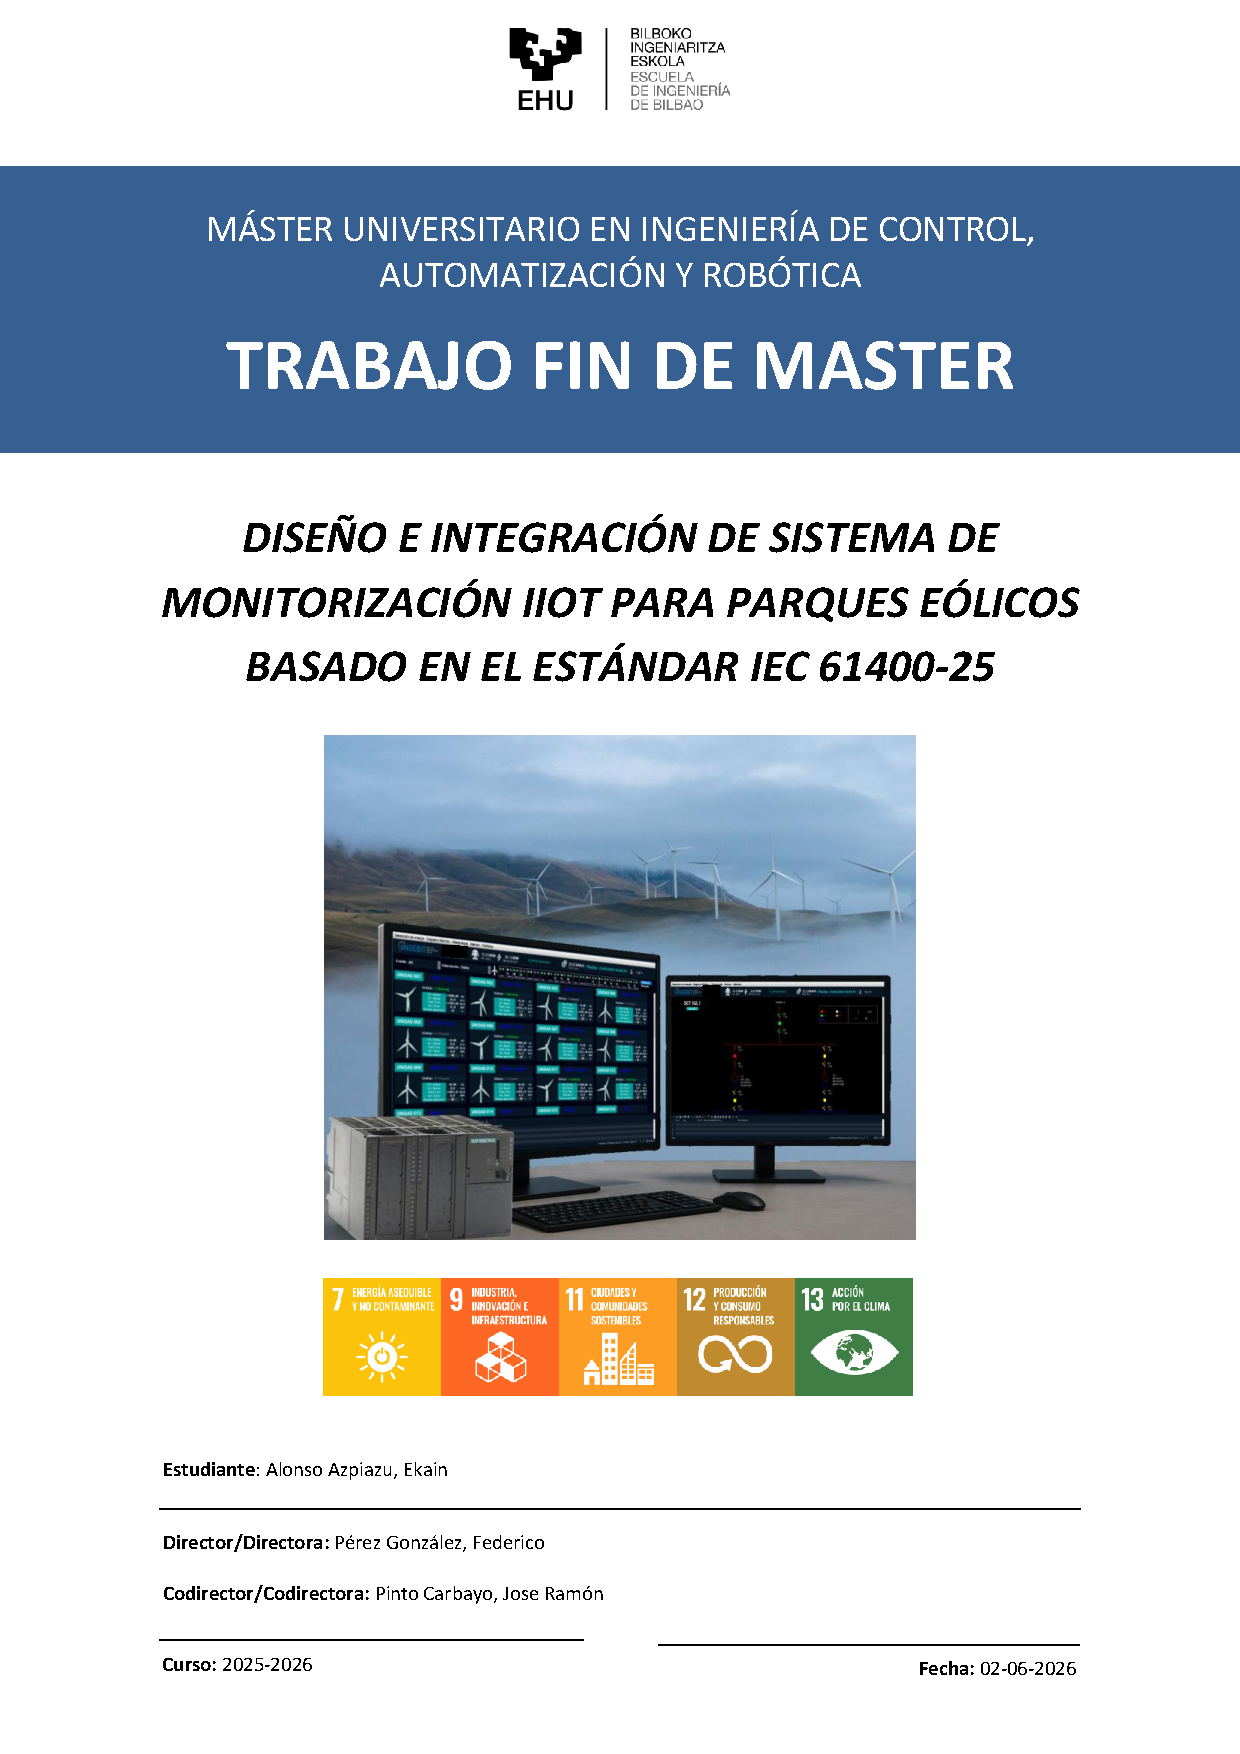
\includepdf[pages=-]{Portada.pdf} % Se recomienda modificar en word y subir el pdf 

%---

%--- Implementar las partes principales del TFM
\pagestyle{plain}
\chapter*{Resumen Trilingüe}
\label{sec:abstract}
\vspace*{-10mm}

\textbf{Resumen}

\textit{"En la última década, la industria ha llevado a cabo una transición acelerada desde arquitecturas centralizadas hacia sistemas de control distribuidos (DCS). Este nuevo estandar, impulsado por la digitalización y la convergencia de las Tecnologías de la Operación (OT) y de la Información (IT), permite crear redes de sistemas ciberfísicos (CPS) escalables sentando las bases de la Industria 4.0. Este cambio es críticamente notable en el sector energético, donde el modelo tradicional de generación de energía, basado en combustibles fósiles en centrales monolíticas, ha dado paso a un sistema más diversificado, sostenible y distribuido (parques eólicos, plantas solares etc.). En este contexto, los sistemas de supervision, control y adquisicion de datos (SCADA) se han consolidado ofreciendo soluciones de conectividad que garantizan la interoperabilidad, seguridad en los CPS. El trabajo de fin de master consiste en una solución SCADA para una red de generación eólica, el cual estará ubicado en una sala de control central (MCR).El desarrollo se fundamenta en la normativa internacional IEC 61400-25 que regula las comunicaciones en parques eólicos. Este sistema SCADA posibilita la gestión de alarmas y eventos, la elaboración de gráficas de tendencia y la ejecución de tareas de mantenimiento predictivo de las instalaciones desde un punto central, mejorando la eficiencia y productividad de toda la red. La memoria recoge además un manual de usuario y un banco de pruebas.}\par

% En Español: 
\textbf{Palabras clave:} Industria 4.0; Sistemas CiberFísicos; Parque Eólico; Energía; Subestaciones eléctricas; Energía sostenible
; OPC UA; Modbus TCP ; mantenimiento; turbinas.

\vspace*{5mm}
\textbf{Abstract}

\textit{In the last decade, the traditional model of power generation, based on centralized fossil fuels, has given way to a more diversified, decentralized, and sustainable system. As the new paradigm becomes established, information management problems arise due to the dispersion of systems. To address the logistics and management issues caused by this dispersion, the master's thesis proposes the design of a supervisory control and data acquisition system (SCADA) supported by the international standard for communication in wind power plants IEC 61400-25, to unify signals and enable the centralized and efficient control that the new distributed generation standard requires. This SCADA system enables alarm and event management, the creation of trend graphs, and the execution of predictive maintenance tasks for installations from a central point, improving the efficiency and productivity of the entire network.}\par

\textbf{Keywords:} xxx
\vspace*{5mm}
\textbf{Laburpena}

Azken hamarkadan, erregai fosil zentralizatuetan oinarritutako energia-sorkutza bide eman dio eredu deszentralizatu batera. Paradigma berria ezartzen den heinean, informazioaren kudeaketan arazoak sortuz joan dira. Master amaierako lanak, energia berriztagarri ekoizpen sare baten kontrol eta kudeaketa gela (MCR) diseinatzen du. Horrela, estazio monolitikoetan tradizionalki zegoen kontrolaren antzeko sistema bat ezartzen da eta kontrol banatuaren arazoari irtenbidea ematen zaio. Gelak gainbegiratzeko kontrol eta datu eskuratze sistema (SCADA) bat eta WIN Server sistema eragileekin bi zerbitzari erreserbatu ditu, eta 20 azpiestazio elektriko eta energia-sorkuntza sistemetako bakoitzarekin komunikatuta dago (122 aerosorgailu eta eguzki-parke), guztira 744 MW energia elektriko kudeatuz. Horrela, MCRk alarmen eta gertaeren kudeaketa, joeren grafikoen prestaketa eta instalazioen mantentze prediktiboko lanak egitea ahalbidetzen du. Azkenik, martxan jartze birtual bat gauzatzen du funtzionamendu egokia bermatzeko.

\textbf{Hitz gakoak:} xxx



%--- Índice general
\cleardoublepage
\renewcommand{\contentsname}{Índice}  % Cambiar el nombre a contenidos
\tableofcontents  % Crear la tabla de contenidos
%---

%--- Índice de figuras
\cleardoublepage
\renewcommand{\listfigurename}{Índice de Figuras}  % Cambiar el nombre al índice de figuras
\addcontentsline{toc}{chapter}{\listfigurename} % Añade la lista de tablas a la Tabla de Figuras
\listoffigures    % Índice de figuras (opcional)
%---

%--- Índice de tablas
\cleardoublepage
\renewcommand{\listtablename}{Índice de Tablas}  % Cambiar el nombre al índice de tablas
\addcontentsline{toc}{chapter}{\listtablename} % Añade la lista de tablas a la Tabla de Contenidos
\listoftables % Índice de tablas (opcional)
%---




\renewcommand{\figurename}{Figura}
%--- Lista de acrónimos
\clearpage

\chapter*{Acrónimos} % Opción con * para que no aparezca en TOC ni numerada
\addcontentsline{toc}{chapter}{Acrónimos} % Añade al TOC.

\begin{acronym}[MPC] % Give the longest label here so that the list is nicely aligned
\acro{INCAR}{Ingeniería de Control, Automatización y Robótica}
\acro{SIVaaS}{Simatic Virtualization as a Service}
\end{acronym}	
\renewcommand{\tablename}{Tabla}
\cleardoublepage
%---

%--- Implementar los capítulos principales del TFM
\pagenumbering{arabic}			
\setcounter{page}{1}			
\pagestyle{maincontentstyle} 	
\chapter{Introducción}
\label{cap:introduccion}
El proyecto se desarrolla en el marco de un trabajo fin de máster dentro del programa de Máster Universitario en Ingeniería de Control, Automatización y Robótica (INCAR) impartido por la Universidad del País Vasco (EHU). El proyecto se desarrolla en la sede de INGEBIT S.L. empresa especializada en ofrecer soluciones en los diferentes ámbitos de la industria 4.0. ubicada en Barakaldo, Bizkaia, España. \par

A inicios de siglo la generación energética en España se basaba principalmente en grandes centrales térmicas y nucleares, con una participación limitada de fuentes renovables. Sin embargo, el auge de la industria 4.0  junto con el creciente problema del cambio climático, ha impulsado que el modelo de generación de energía tradicionalmente monolítico pase a sistemas de generación sostenibles. Estos sistemas son de menor potencia de generación por lo que se requiere un mayor volumen y distribución de ellos.\par

En este contexto, este trabajo fin de máster consiste en el diseño e implementación de un sistema SCADA para la gestión integral de una red de generación de energía sostenible. El sistema permitirá la monitorización centralizada, el control automatizado y la optimización de recursos energéticos, incorporando capacidades de mantenimiento predictivo basadas en análisis de datos en tiempo real.\par

El proyecto se divide en varias fases, incluyendo la planificación, el diseño del sistema SCADA, la implementación y las pruebas finales. Durante el desarrollo  se aplican los conocimientos adquiridos a lo largo del máster, así como las habilidades técnicas y de gestión de proyectos necesarias para llevar a cabo un proyecto de esta envergadura.\par
\chapter{Contexto}
\label{cap:contexto}

En el contexto se presenta el ámbito en el que se ha desarrollado el TFM.
Considerar hablar desde aspectos más generales, a aquellos más
particulares relacionados con el TFM. Finalizar con un párrafo que hable de la problemática en la cual se ha focalizado el TFM detallando la necesidad de profundizar en esa área de investigación.

\section{Marco Macroscópico: La Descentralización del Sector Energético}
\label{sec:marco_macroscopico}

El presente Trabajo de Fin de Máster se contextualiza en el escenario global de la transición energética y la digitalización industrial, un proceso caracterizado por la migración activa desde un modelo de generación eléctrica centralizado basado en combustibles fósiles hacia un ecosistema distribuido y bajo en carbono. Este cambio de paradigma está impulsado por políticas internacionales de descarbonización y por planes estratégicos que imponen un despliegue masivo de fuentes de energía renovables \cite{aee2026}.Las directrices globales de descarbonización se rigen por el marco jurídico internacional del Acuerdo de París \cite{unfcccParisAgreementPub}, el cual establece el límite del incremento térmico en 1.5~°C. Los escenarios de descarbonización global exigen triplicar la capacidad instalada de energías renovables y optimizar las redes de distribución para absorber la generación distribuida, fijando marcas hacia el año 2030 \cite{ieaNetZero2023Update}.

En España el proceso de transición energética se enmarca dentro del Plan Nacional Integrado de Energía y Clima (PNIEC) 2021--2030 \cite{mitecoPNIEC2023}, el cual establece objetivos vinculantes para la reducción de emisiones de gases de efecto invernadero (GEI) en un 23\% para el año 2030 respecto a los niveles de 1990, con una meta específica de alcanzar una potencia instalada de energías renovables de 74~GW. Requiriendo una gestión eficiente que garantice la estabilidad y seguridad del sistema eléctrico nacional.\par

\section{Marco Microscópico: La Complejidad de la Gestión de Parques Eólicos}
Desde la perspectiva de la automatización, la transición hacia las energías renovables introduce una complejidad de campo. Mientras que una central térmica tradicional concentra una elevada potencia en un único punto monolítico, un parque eólico moderno fragmenta dicha potencia en decenas de activos individuales (aerogeneradores) distribuidos a lo largo de amplias extensiones geográficas. Cada una de estas turbinas constituye un sistema ciberfísico (CPS) complejo, dotado de su propia instrumentación, electrónica de potencia y lazos de control internos en tiempo real (regulación de orientación, paso de pala y par del generador). En adición la integración de activos de diferentes fabricantes o generaciones tecnológicas introduce una heterogeneidad de protocolos y estructuras de datos que dificulta la supervisión unificada. Por ello se han desarollado estandares internacionales de interoperabilidad como la norma IEC 61400-25 o la norma IEC 61850 \cite{vattenfall61400} \cite{iec61400-25}.



\section{Ámbito Operativo: La Sala de Control Principal (MCR)}
\label{sec:ambito_operativo_mcr}

Ante la imposibilidad de operar eficientemente cientos de infraestructuras dispersas mediante intervenciones locales, el sector eólico ha centralizado su gestión en las denominadas de Organización y Mantenimiento  (O and M). El ámbito en el que se encuadra este TFM emula de forma directa el entorno de ingeniería de una MCR corporativa, cuyo propósito es unificar bajo una misma capa de software la adquisición de datos y el diagnóstico de múltiples parques eólicos y sus respectivas subestaciones eléctricas de evacuación.

\chapter{Objetivos y alcance}
\label{cap:objetivos}

\section{Objetivos}

El objetivo general de este proyecto de fin de master es diseñar e implementar una solución de supervisión y control de parques eólicos, con un enfoque específico en la integración de datos siguiendo el estándar internacional IEC 61400-25 y la norma matriz IEC 61850,  integrando además las tecnologías \ac{IT} mediante el internet industrial de las cosas (\ac{IIoT}). Para alcanzar este objetivo general, se han definido los siguientes objetivos específicos:
\begin{itemize}

\item  Objetivo 1: analizar los requisitos funcionales y no funcionales de un sistema de monitorización para parques eólicos, considerando aspectos como la cantidad de turbinas a manejar, la arquitectura del sistema y las especificaciones de comunicación. Además de realizar un estudio de software de desarrollo de la solución.  
\item  Objetivo 2: diseñar el \ac{IM} de la planta eólica basado en el estándar IEC 61400-25-2 y de las subestaciones eléctricas según el estándar IEC 61850. Para ello, se definirá la estructura de datos, las variables de proceso y los atributos necesarios para representar la telemetría de las turbinas y la subestación eléctrica. Diseñar la  jerarquía y navegación de pantallas y realizar la conectividad con la nube para la visualización de datos en tiempo real. 

\item  Objetivo 3: diseñar e implementar un banco de pruebas con la finalidad de simular el comportamiento tanto de las turbinas como de las subestaciones eléctricas de las que cuelgan. Este banco de pruebas se utilizará para validar la correcta implementación del modelo de información y la funcionalidad del sistema de supervisión desarrollado.

\end{itemize}


\section{Alcance}

El presente trabajo abarca la definición, diseño y construcción de un prototipo funcional de supervisión orientado a parques eólicos, prestando especial atención a la especificación del modelo de información, la interoperabilidad entre equipos y la integración con servicios en la nube. La solución se orienta exclusivamente a la visualización y monitorización del estado de los activos: no contempla el envío de consignas de control ni la ejecución de órdenes de mando desde el SCADA hacia las turbinas o la subestación. Como resultados concretos se entregarán el modelo de información detallado, un banco de pruebas para la simulación de turbinas y subestaciones, y la documentación técnica necesaria para la replicación y adaptación de la solución.\par

El trabajo contemplará además la verificación funcional mediante casos de prueba y procedimientos de validación ejecutables en el banco de pruebas; se evaluarán criterios básicos de rendimiento, escalabilidad y robustez (por ejemplo latencia de adquisición, integridad de datos y capacidad de añadir nuevos nodos), y se redactarán recomendaciones para mitigación de riesgos y consideraciones de ciberseguridad aplicables a escenarios de despliegue.\par

Quedan fuera del alcance las actividades de control de instalación física, puesta en marcha en campo y operación continuada en un emplazamiento productivo.\par

\chapter{Beneficios}
\label{cap:beneficios}

Describir los beneficios que aporta el trabajo realizado:  beneficios tecnológicos, económicos, sociales, etc.

\chapter{Análisis del estado del arte}
\label{cap:estado_del_arte}


 


% En Español: 
\section{Introducción}

% En Ingles: 
%\section{INTRODUCTION}
\par
La implementación de sistemas de control de supervisión y adquisición de datos (\ac{SCADA}) constituye un elemento esencial dentro de los procesos de automatización industrial, ya que permite no solo recopilar y archivar información, sino también visualizarla, transmitirla y gestionarla de manera eficiente, asegurando así un control integral de las operaciones. En el ámbito de la generación eléctrica, estos sistemas se han consolidado como herramientas imprescindibles para optimizar tanto la eficiencia como el mantenimiento de grandes aerogeneradores, además de facilitar la gestión de las subestaciones eléctricas asociadas. A partir de los avances alcanzados en los últimos años, la investigación académica ha orientado sus esfuerzos hacia la mejora de la eficiencia en la producción energética y la resolución de los problemas derivados de la creciente descentralización de los sistemas de generación.\par


\subsection{Arquitecturas inalámbricas en parques eólicos}
Un enfoque de creciente interés dentro del estado del arte se centra en la flexibilización y modernización de la infraestructura de comunicaciones mediante el despliegue de redes inalámbricas bajo el paradigma de los Sistemas Ciberfísicos (CPS). Autores como Ahmed et al. \cite{Ahmed2020} \cite{ahmed2014communication} defienden que las soluciones inalámbricas estructuradas de forma jerárquica y basadas en el estándar IEC 61400-25 segmentando el tráfico en redes internas de la turbina (WTIN), perimetrales (WTAN) y globales del parque (WFAN) superan las limitaciones de los sistemas convencionales cableados al reducir drásticamente los costes de instalación y ofrecer topologías dinámicas y escalables, especialmente viables en entornos remotos o de orografía compleja \cite{gungor2009industrial}. En sus investigaciones, mediante simulaciones de flujos de datos analógicos de alta frecuencia, demuestran que tecnologías como Wi-Fi y ethernet no solo son viables, sino que logran cumplir con los estrictos requisitos de retardo extremo a extremo, relegando a tecnologías de bajo ancho de banda como ZigBee a telemetrías secundarias\cite{mahmood2015review}.\par  

\begin{figure}[tb]
    \begin{subfigure}{0.3\textwidth}
        \centering
        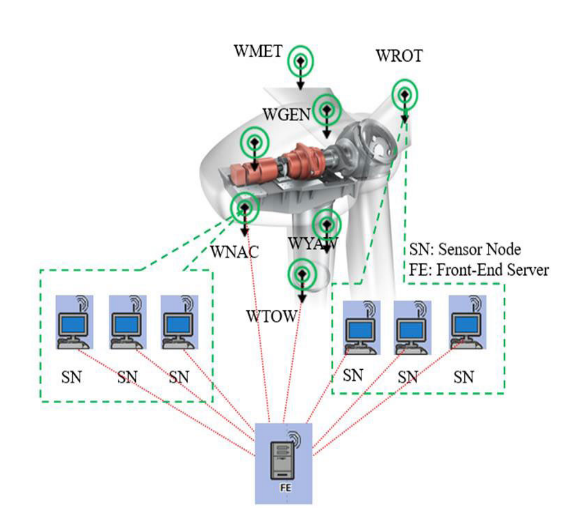
\includegraphics[width=\textwidth,height=0.8\linewidth]{figuras/Wifi.png}
        \caption{Arquitectura de red inalámbrica en parques eólicos.}
        \label{fig:wifi}
    \end{subfigure}
     \begin{subfigure}{0.3\textwidth}
        \centering
        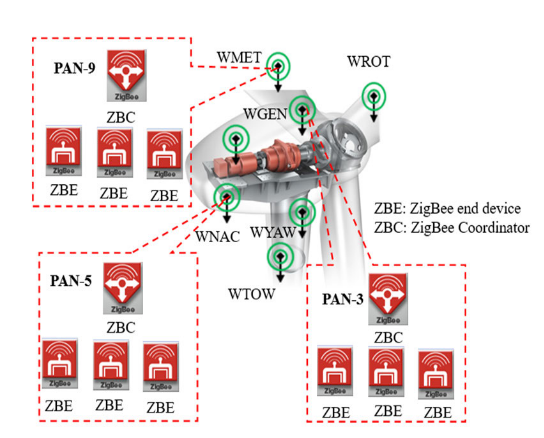
\includegraphics[width=\textwidth,height=0.8\linewidth]{figuras/zigbee.png}
        \caption{Arquitectura de red inalámbrica ZigBee en parques eólicos.}
        \label{fig:zigbee}
    \end{subfigure}
    \begin{subfigure}{0.3\textwidth}
        \centering
        \includegraphics[width=\textwidth,height=0.8\linewidth]{figuras/ethernet.png}
        \caption{Arquitectura de red cableada con ethernet en parques eólicos.}
        \label{fig:ethernet}
    \end{subfigure}
    \caption{Comparativa de arquitecturas inalámbricas en aerogeneradores. Obtenido de \cite{Ahmed2020}}
\end{figure}

Sin embargo, desde una perspectiva de operación crítica en el sector eléctrico, las tecnologías inalámbricas introducen incertidumbres asociadas a la pérdida de determinismo y la vulnerabilidad ante interferencias electromagnéticas severas, habituales en el entorno perimetral de un aerogenerador.\par

\subsection{Ciberseguridad en sistemas \ac{SCADA} de parques eólicos}
Por otra parte, la creciente necesidad de interoperabilidad entre sistemas empuja a que los \ac{SCADA} se diseñen para facilitar el acceso externo a la información sin comprometer la seguridad operativa. En lo que respecta a la exposición segura de variables operacionales hacia el exterior, el estado del arte marca la importancia de la segmentación de red en infraestructuras eólicas distribuidas. Autores como Shih abordan este desafío en entornos de parques eólicos marinos mediante el despliegue de \ac{DMZ} combinadas con el protocolo de telecontrol IEC 60870-5-104 \cite{Shih2022}. La arquitectura de Shih demuestra que interponer una \ac{DMZ} resguarda eficazmente la red local de control \ac{OT} frente a intrusiones externas, permitiendo que terceras entidades consulten históricos de viento y generación sin comprometer la estabilidad de los activos.\par

No obstante, el despliegue de una \ac{DMZ} local compleja requiere servidores e infraestructura de red replicada en planta para aislar el tráfico. En lugar de ello se puede utilizar el protocolo \ac{MQTT} nativo desde un \ac{SCADA} debido a su naturaleza unidireccional y basada en publicaciones y de poca latencia \cite{ferrari2020evaluation}. Con \ac{MQTT}, es el propio nodo perimetral de la planta (Edge) el que abre de forma segura una única conexión saliente \ac{TCP} hacia un bróker en la nube para publicar los datos. Al no requerir puertos de entrada abiertos en la red local de operaciones (OT), se elimina superficie para un ciberataque, simplificando la arquitectura de ciberseguridad sin perder visibilidad.\par

\subsection{Mantenimiento predictivo y predicción de potencia mediante inteligencia artificial}
Más allá de la transmisión de datos, uno de los retos más relevantes en la gestión de parques eólicos es la predicción de la potencia generada. Tradicionalmente, esta se estima mediante curvas de potencia obtenidas a partir de técnicas de reducción de datos como el \textit{binning}, en el que se agrupan las velocidades de viento y las densidades del aire en intervalos específicos. Sin embargo, el aumento en el tamaño de las turbinas hace que fenómenos como la cizalladura del viento o la intensidad de las turbulencias tengan un impacto mayor en la curva, al utilizar datos históricos meteorológicos recopilados por un sistema \ac{SCADA} se pueden mejorar significativamente las predicciones clásicas \cite{Pandit2023}.

El mantenimiento predictivo se ha consolidado como uno de los principales beneficios de los sistemas \ac{SCADA}, ya que permite anticipar fallos, reducir costes operativos y garantizar la seguridad tanto de los trabajadores como de las infraestructuras, por ejemplo, tras el impacto de un rayo en una pala de aerogenerador para determinar el grado de daño \cite{Matsui2021}. También se puede utilizar para la predicción de fallos por desgaste y en la construcción de modelos de diagnóstico basados íntegramente en datos de salud de aerogeneradores \cite{Khan2024} \cite{Shi2021}.

En terrenos muy complejos, asumir que todas las turbinas sufren las mismas condiciones ambientales no es realista ya que varían significativamente entre turbinas. Los métodos tradicionales confunden estas variaciones (o paradas manuales) con fallos mecánicos. Por ello, existen soluciones dónde en lugar de agrupar todas las turbinas o un grupo menor por distancia física, se agrupan por similitud en condiciones externas. En estas soluciones, El \ac{SCADA} proporciona las variables ambientales críticas al algoritmo de clasificación necesarias para agrupar las turbinas correctamente, lo que ayuda a detectar fallos graves con meses de antelación sin generar falsas alarmas (ver figura \ref{fig:ml}), incluso en parques eólicos con orografía difícil \cite{Du2023}.

\begin{figure}[tb]
    \centering
    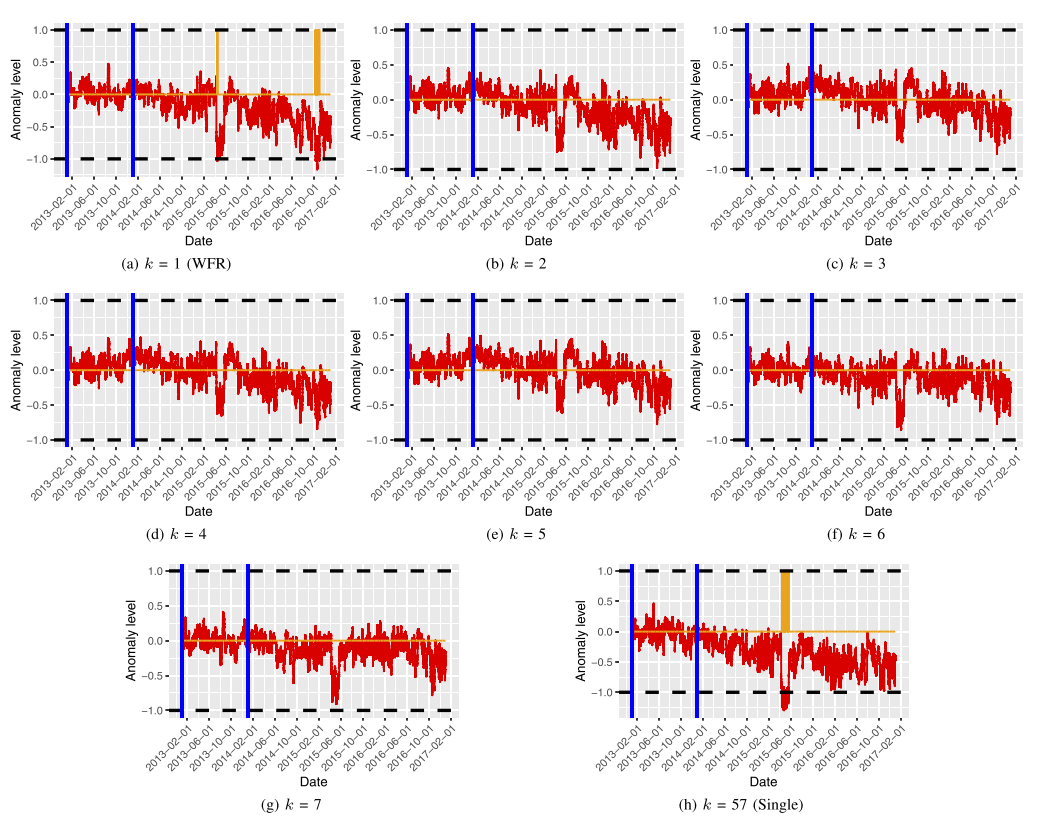
\includegraphics[width=\textwidth]{figuras/Anomalia.png}
    \caption{Evolucion de las falsas alarmas (naranja) en un parque eolico agrupando los aerogeneradores en grupos de condiciones (k-means) en lugar de por proximidad física \cite{Du2023}.}
    \label{fig:ml}
\end{figure}

Finalmente, la irrupción de las tecnologías de aprendizaje automático y profundo ha ampliado de manera significativa las posibilidades del mantenimiento predictivo. Algunos estudios emplean arquitecturas de \ac{CNN} para extraer patrones dinámicos de los datos de turbinas \cite{Kong2020} \cite{Xiang2021}, mientras que otros exploran modelos LSTM y regresiones para anticipar fallos en las curvas de potencia \cite{Udo2021}. Sin embargo, su efectividad depende intrínsecamente de la arquitectura de supervisión que se encarga de recoger los datos. Lo que revaloriza el diseño del sistema \ac{SCADA} como la infraestructura crítica e indispensable. Solo mediante un sistema de adquisición de calidad es posible alimentar estos algoritmos para optimizar la vida útil de los componentes, reducir costes y mejorar la fiabilidad del sistema.\par

\section{Conclusiones del estado del arte}
En conclusión, la eficacia de las técnicas avanzadas de predicción y mantenimiento dependen intrínsecamente de la calidad de la adquisición de datos. Esta base es el pilar de la gestión eficiente de parques eólicos, en las que tecnologías como la \ac{IA} y el \ac{ML} se sustentan para obtener predicciones precisas. Por todo esto, el desarrollo de un sistema de supervisión y adquisición de datos (\ac{SCADA}) eficiente, robusto y ciberseguro capaz además de alimentarse de plantas en cualquier entorno es indispensable para desarrollar e implementar las tecnologías emergentes para el mantenimiento predictivo del futuro, junto con las necesidades del sector energético. Lo que motiva el trabajo desarrollado en este TFM. \par

\chapter{Análisis de alternativas}
\label{cap:soa}

Análisis de alternativas y selección de elementos necesario para la ejecución del TFM.
\chapter{Diseño/Desarrollo de la solución}
\label{cap:desarrollo_de_la_solucion}

\section{Introducción al entorno de SIMATIC WinCC V8.1}
SIMATIC WinCC V8.1 es un sistema SCADA, basado en los sistemas operativos Microsoft Windows, desarrollado por Siemens AG. Está diseñado para la visualización, control y operación de procesos, flujos de producción, máquinas y plantas críticas en diversos sectores industriales.

\par \indent WinCC actúa como una Interfaz Hombre-Máquina (HMI) de alto nivel. A diferencia de los paneles de operador básicos ubicados a pie de máquina, un HMI de alto nivel como WinCC proporciona un entorno gráfico avanzado que abstrae la complejidad de los equipos físicos. Esto permite a los operadores del centro de control manejar, monitorizar y entender de forma intuitiva los procesos dinámicos que se ejecutan en la planta sin tener que estar en la ubicación de la máquina. La comunicación entre el entorno de supervisión WinCC y la maquinaria física se efectúa de manera bidireccional a través de sistemas de automatización, empleando protocolos de comunicación industrial.(\ref{fig:wincc_interface})

\begin{figure}[t]
    \centering
    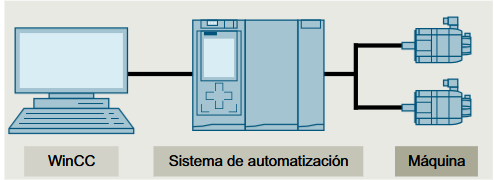
\includegraphics[scale=0.8]{figuras/WinCC.png}
    \caption{Ejemplo de interfaz gráfica de WinCC V8.1. Fuente: Siemens}
    \label{fig:wincc_interface}
\end{figure}

\par \indent Por otro lado, WinCC es plataforma altamente programable. Integra un motor de ejecución que permite la creación de lógicas complejas y automatización de tareas de supervisión utilizando interfaces de aplicación  como ANSI-C y VBScript (Visual Basic).Por otro lado, WinCC V8.1 utiliza de forma nativa el motor de bases de datos Microsoft SQL Server. Este gestor de bases de datos opera en segundo plano y se encarga del archivado histórico continuo de las variables del proceso y del registro de eventos y fallos.

\par \indent Desde el punto de vista de la arquitectura de software, el entorno de WinCC se divide en dos componentes fundamentales y complementarios: el sistema de configuración o Configuration Software (CS) y el entorno de ejecución o Runtime (RT):
\subsection{Software de configuración (SC) WinCC Explorer}
El software de configuración se denomina WinCC Explorer. En él se realiza toda la estructura y administración del proyecto. Dentro del WinCC Explorer se pueden abrir diferentes editores los cuales son interfaces de los subsistemas de WinCC \ref{tab:wincc_subsystems}. 
\begin{table}[t]
    \centering
    \caption{Descripción de los subsistemas principales del software de configuración de WinCC (\textit{CS}).}
    \begin{tabular}{p{5cm} p{3cm} p{6cm}} 
            \toprule
        	\textbf{Subsistema} & \textbf{Editor} & \textbf{Descripción} \\ 
        \hline
        Sistema gráfico & Graphic Designer & Diseño de las pantallas de visualización \\
        Comunicación & Tag management & Creación de variables (internos o de estructura) configuración de drivers de comunicación y conexión con los datos del proceso \\[10pt]
        Sistema de ficheros & Tag logging & Administración de archivado de datos historicos \\[10pt]
        Sistema de avisos & Alarm logging & Gestión de alertas y eventos \\[10pt]
        Sistema de informes & Report Designer& Creación y gestión de informes \\[10pt]
        Administración de usuarios & User Administrator& Gestión de usuarios, grupos y sus respectivos permisos\\[10pt]
        Subsistema de Scripts & Global Scripts & Diseño de Scripts globales del programa (Visual Basic VBS/ ANSI-C) \\[10pt]
        Gestión de idiomas & Text library & Configuración y gestión de idiomas \\[10pt]
        \bottomrule
    \end{tabular}
    \vspace{0.5cm}
    
    \label{tab:wincc_subsystems}
\end{table}

\subsection{Software \textit{Runtime (RT)}: WinCC Runtime}
El WinCC RT constituye el núcleo operativo del SCADA. Durante la operación normal del proceso, el Runtime es el motor encargado de ejecutar la adquisición de datos de los PLCs en tiempo real, actualizar dinámicamente la interfaz gráfica, procesar la lógica de los scripts, gestionar el control de acceso de los usuarios y archivar de manera segura los eventos y datos históricos en las bases de datos SQL.\par

\section{Arquitecturas del sistema}
\subsection{Topología de red del parque eólico y MCR}
\subsection{Arquitectura de WinCC}
El diseño de una red SCADA determina la forma en la que se hace la adquisición, procesamiento y visualización de datos. El entorno de Siemens permite multiples arquitecturas y configuraciones de proyecto dependiendo del tipo de sistema
\subsubsection{Sistemas Monopuesto (\textit{Single User Systems})}
En la arquitectura de sistema monopuesto un único equipo físico o estación se encarga de realizar todas las tareas del SCADA. El puesto actúa tanto como servidor como cliente: El equipo se encarga de realizar las comunicaciones con la parte operativa (mediante los protocolos de comunicación como Profinet o ModBus, OPC UA …) de ejecutar el software del runtime y almacenar los históricos y alarmas en la base de datos SQL a la vez que muestra la interfaz gráfica al operario en los monitores. \par
Para este tipo de sistemas Siemens ofrece dos arquitecturas posibles: La primera se trata de una estación de ingeniería y runtime con un único PC (Figura \ref{fig:monopuesto}). La segunda, es una configuración redundante de la primera donde la estación redundante solo sería una estación runtime (Figura \ref{fig:monopuesto_redundante}).

\begin{figure}[t]
    \centering
    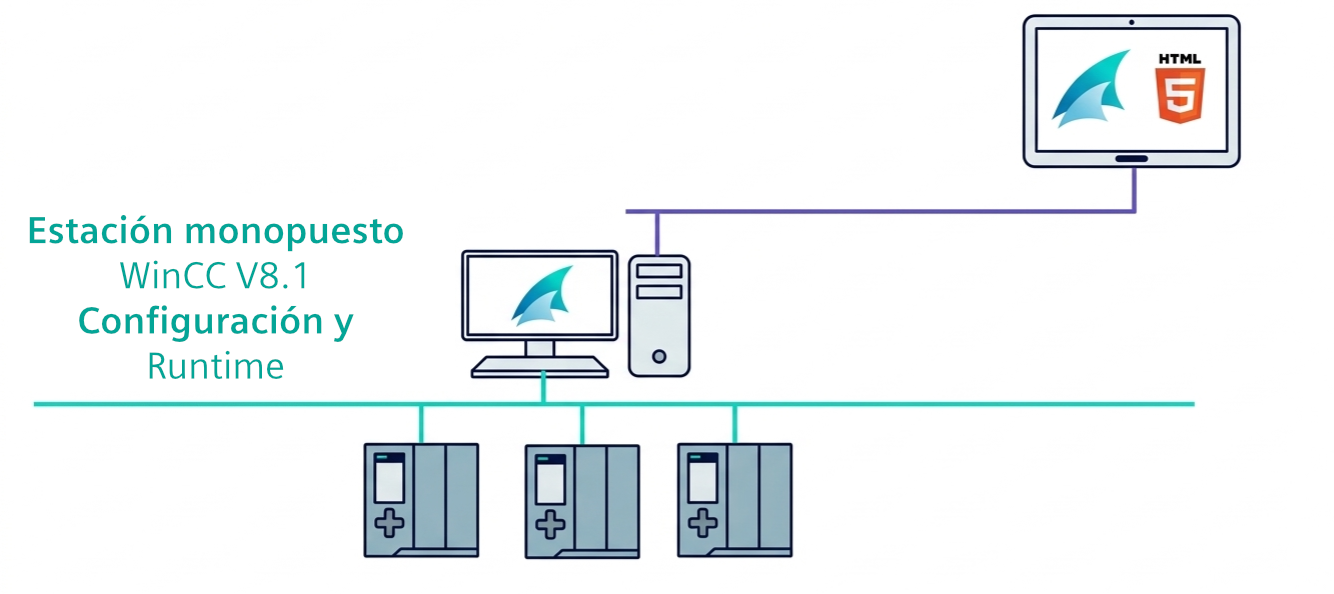
\includegraphics[scale=0.3]{figuras/Monopuesto.png}
    \caption{Arquitectura de sistema monopuesto con un único PC}
    \label{fig:monopuesto}
\end{figure}

\begin{figure}[t]
    \centering
    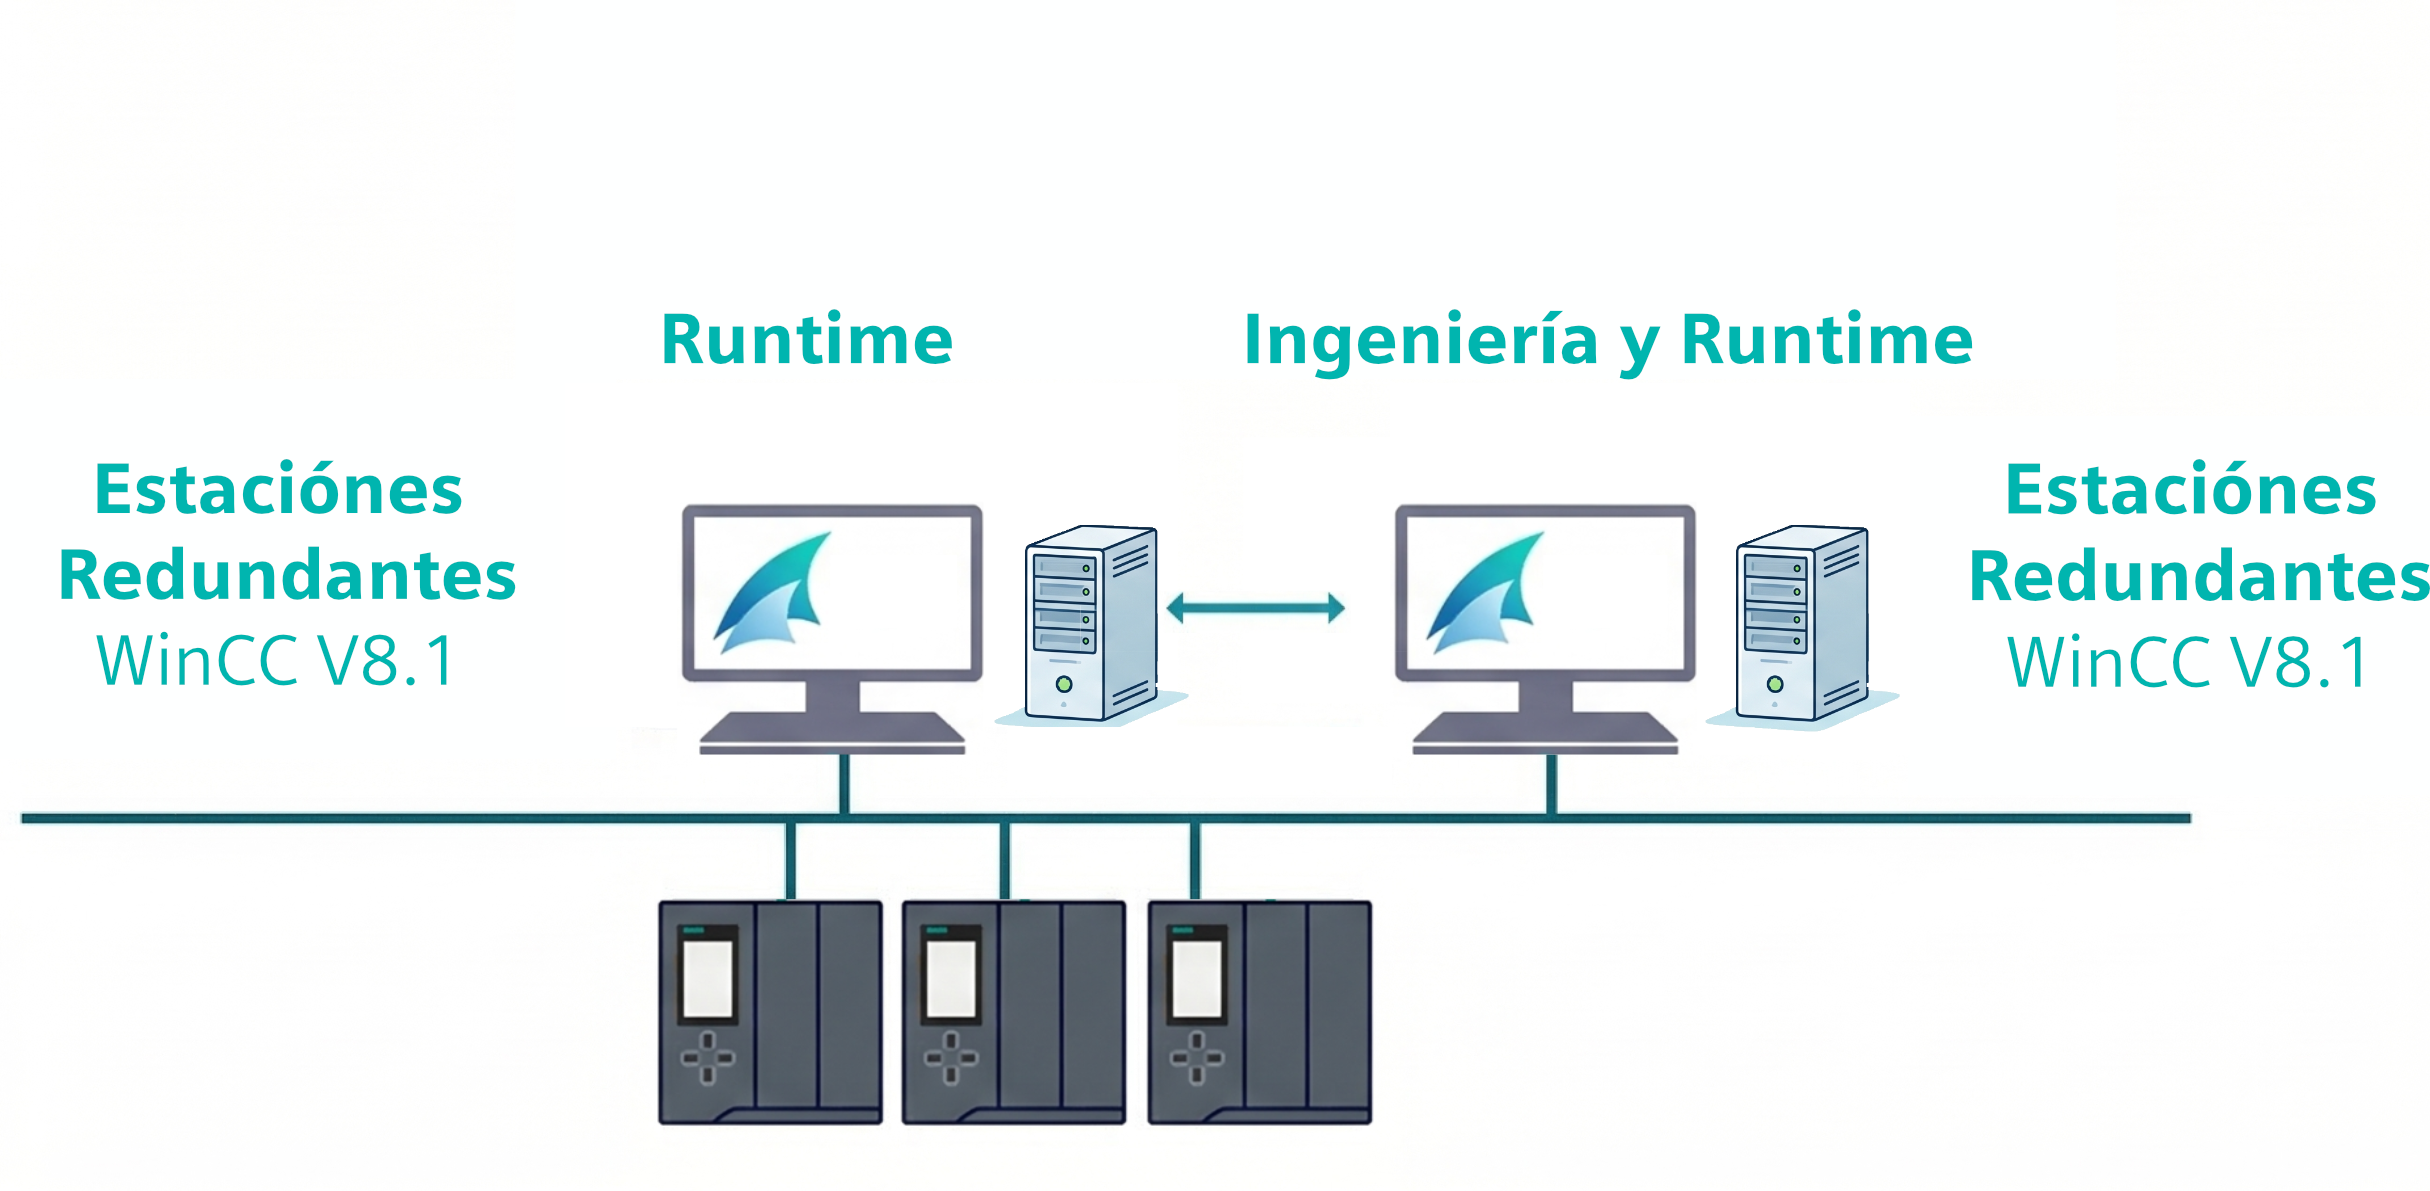
\includegraphics[scale=0.15]{figuras/MonopuestoRedundante.png}
    \caption{Arquitectura de sistema monopuesto con configuración redundante}
    \label{fig:monopuesto_redundante}
\end{figure}

\subsubsection{Sistemas Multipuesto (\textit{Multi User Systems})}


Un sistema multipuesto es una arquitectura distribuida diseñada para separar las tareas de procesamiento de datos de las tareas de visualización. A diferencia de un sistema monopuesto (donde un solo ordenador hace todo), en un sistema multipuesto la carga de trabajo se divide entre uno o varios Servidores centrales y múltiples estaciones Cliente. Este enfoque permite una variedad mayor de arquitecturas y configuraciones de proyecto, adaptándose a las necesidades específicas de cada instalación. ( Figura \ref{fig:multipuesto}) \par 
\begin{figure}[t]
    \centering
    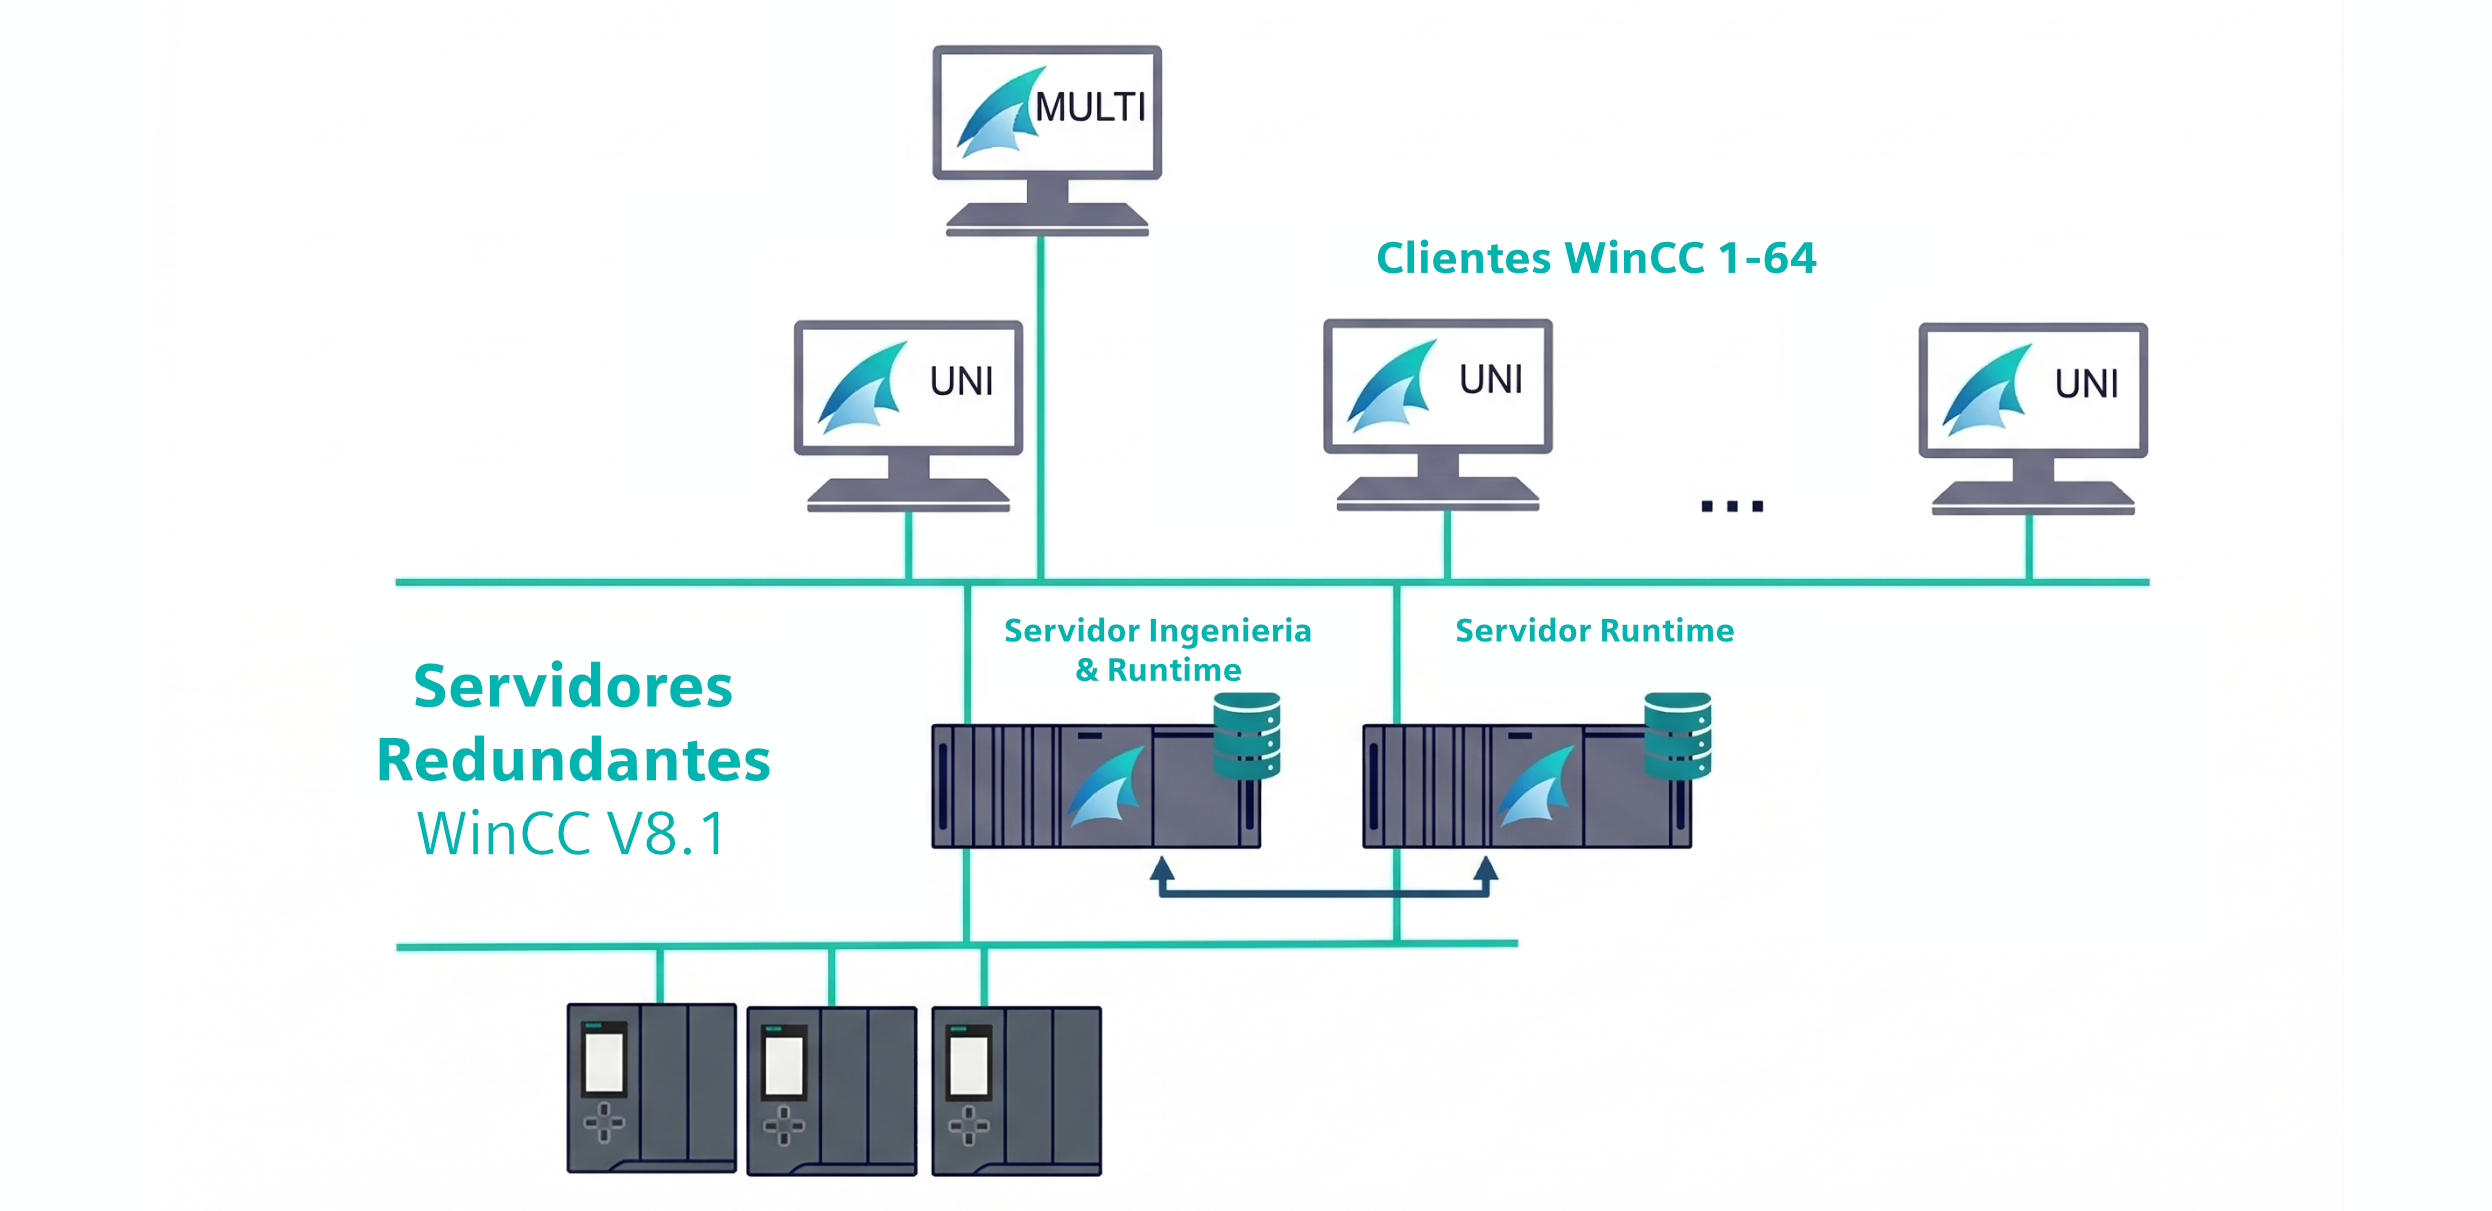
\includegraphics[scale=0.17]{figuras/Multipuesto.png}
    \caption{Ejemplo de arquitectura de sistema multipuesto: Dos servidores centrales redundantes, el primero Runtime y el segundo ingeniería y Runtime conectados a múltiples estaciones cliente.}
    \label{fig:multipuesto}
\end{figure}
\subsubsection{Virtualización mediante SIVaaS}

La virtualización es un método por el que los recursos físicos de un equipo se pueden dividir en diversos entornos virtuales. Para ello se utiliza un hipervisor que se encarga de ejecutar múltiples máquinas virtuales (VM) aisladas, compartiendo recursos como CPU, memoria y almacenamiento. Este aislamiento evita los conflictos debidos a las dependencias de software y proporciona la capacidad de iniciar y detener las máquinas virtuales de forma independiente. Solo la máquina virtual en cuestión se ve afectada por un fallo (o caída del sistema). Existen dos tipos de hipervisores: Alojados y Metal-Desnudos.
\paragraph{Hypervisor alojado  (\textit{Hosted Hypervisor})}
Este tipo se instala como una aplicación de software más dentro de un sistema operativo convencional que ya está funcionando en el equipo físico (conocido como sistema operativo anfitrión u Host OS).\par

Este tipo de hipervisor genera una dependencia del sistema operativo base ya que el hipervisor debe pedir constantemente permiso para acceder a los recursos del sistema lo cual genera un cuello de botella disminuyendo el rendimiento. \par

Por otro lado, esta dependencia del sistema operativo base es una vulnerabilidad en sí misma para la seguridad y ciberseguridad del sistema, ya que un malfuncionamiento o un virus podrían contagiarse a cada una de las instancias de maquinas virtuales que corren encima.

\paragraph{Hypervisor metal desnudo (\textit{Bare-Metal Hypervisor})}

Se le denomina Bare-Metal (metal desnudo) porque se instala y ejecuta directamente sobre el hardware físico del servidor. No hay ningún sistema operativo tradicional (como Windows Server o Linux) actuando como intermediario. El hipervisor en sí mismo es un sistema operativo altamente especializado y minimalista diseñado con un único propósito: gestionar y asignar recursos físicos a las máquinas virtuales. Al no tener que atravesar ningún sistema operativo anfitrión, las maquinas virtuales tienen acceso más directo a los recursos del sistema reduciendo la latencia y sobrecarga. \par

Al contrario que un hipervisor alojado, es seguro ante vulnerabilidades, debido a que que tiene una superficie de ataque reducida. Además, las máquinas virtuales están aisladas por lo que si una maquina virtual se ve comprometida por un malware el resto de maquinas permanecerán seguras.\par

\paragraph{Virtualización SIMATIC como Servicio (SIVaaS)}
Siemens ofrece una solución de virtualización completa para sistemas de control basada en hipervisores bare-metal llamada Virtualización SIMATIC como Servicio (SIVaaS). SIVaaS es una solución de virtualización completa para sistemas de control basados en PC. El hardware, el software, la configuración y los servicios de ciclo de vida están totalmente integrados, abarcando desde la configuración del host y el hipervisor hasta las máquinas virtuales, los sistemas operativos y la instalación de software llave en mano. 
Configuración SIVaaS, dos servidores redundados 16X1 HPE HOST SYSTEM "S" con dos máquinas virtuales una haciendo de servidor y la otra de cliente. \par


\begin{table}[t]
    \centering
    \caption{Inserta aquí la descripción de la tabla.}
    \begin{tabular}{p{11cm} p{2cm}}
        \toprule
        \multicolumn{2}{c}{\textbf{Primera instancia de Host}} \\
        \midrule
        Nombre & Cantidad \\
        \midrule
        16X1 HPE HOST SYSTEM "S" & 1\\
        \hline
        \multicolumn{2}{c}{\textbf{Maquinas Virtuales}} \\
        \hline
        VM SIMATIC WinCC V8 Server & 1\\
        VM SIMATIC WinCC V8 Engineering Station + Client & 1\\
        \bottomrule
    \end{tabular}
    \vspace{0.5cm}
    
    \label{tab:Equipo 1}

    \centering
    \caption{Equipo 2: Segunda instancia de Host con dos máquinas virtuales, una haciendo de servidor y la otra de cliente.}
    \begin{tabular}{p{11cm} p{2cm}}
        \toprule
        \multicolumn{2}{c}{\textbf{Segunda instancia de Host}} \\
        \midrule
        Nombre & Cantidad \\
        \midrule
        16X1 HPE HOST SYSTEM "S" & 1\\
        \hline
        \multicolumn{2}{c}{\textbf{Maquinas Virtuales}} \\
        \hline
        VM SIMATIC WinCC V8 Server & 1\\
        VM SIMATIC WinCC V8 Client & 1\\    
        \bottomrule
    \end{tabular}
    \vspace{0.5cm}
    
    \label{tab:Equipo 2}

    \centering
    \caption{Equipo 3: Clientes ligeros para la solución virtualizada.}
    \begin{tabular}{p{11cm} p{2cm}}
        \toprule
        \multicolumn{2}{c}{\textbf{Clientes ligeros}} \\
        \midrule
        Nombre & Cantidad \\
        \midrule
        IGEL OS Thin Client HP T655 Dual Screen INT& 1\\
        Management Console HP T655 Dual Screen WIN10 DE & 1\\
        \bottomrule
    \end{tabular}
    \vspace{0.5cm}
    \label{tab:Equipo 3}
\end{table}



\section{Comunicación y adquisición de datos}
Para la adquisición de datos el entorno de WinCC V8.1 ofrece drivers con una amplia variedad de protocolos y estandares de comunicación industrial como  Open Platform Communication Unified Architecture (OPC UA). 

\subsection{OPC UA}
OPC UA es una tecnología middleware orientada a servicios (SOA). Se divide en dos modelos: El modelo de información y el modelo de comunicación. El modelo de información define cómo se estructuran y organizan los datos dentro del sistema, mientras que el modelo de comunicación establece los protocolos y mecanismos para la transferencia de datos entre los diferentes componentes del sistema. OPC UA es un estándar abierto y multiplataforma que permite la interoperabilidad entre dispositivos y sistemas de diferentes fabricantes. OPC UA incorpora características avanzadas de seguridad, como autenticación, autorización y cifrado, para proteger la integridad y confidencialidad de los datos transmitidos.\par

El envio de mensajes OPC UA se realiza mediante un modelo de publicación-suscripción (pub/sub) donde los dispositivos publican datos en el espacio de direcciones especificando el nodo. En el contexto de la solución WinCC actua de cliente OPC UA, suscribiéndose a los nodos del servidor OPC UA para recibir actualizaciones en tiempo real de las variables del proceso.\par

El servidor OPC UA se desarrolla mediante la herramienta KEPServerEX, la cual permite configurar un servidor OPC UA. Al igual que en Modbus TCP, los valores del proceso se simulan mediante NodeRed. El cliente OPC UA NodeRed publica los datos en el servidor WinCC se suscribe a los nodos simulados por Node Red para recibir las actualizaciones de las variables del proceso en tiempo real.\par

\section{Manejo de Variables}
Las variables en winCC se dividen en tres categorías principales: Variables internas, variables externas y variables de estructura. Las variables internas son aquellas que se crean y gestionan dentro del entorno de WinCC, mientras que las variables externas son aquellas que se adquieren a través de la comunicación con los dispositivos físicos o sistemas externos. Las variables de estructura, por otro lado, son aquellas que siguen una estructura específica definida  para garantizar la interoperabilidad entre diferentes sistemas y dispositivos de tal forma que se mantiene un orden lógico.
\subsection{Variables internas}
El entorno de SIMATIC WinCC V8.1 ofrece una lista de variables internas predeterminadas que se utilizan para diversas funciones dentro del sistema SCADA. Estas variables internas se dividen en diferentes categorías según su función y propósito. Algunas de las categorías principales de variables internas en WinCC incluyen:
\subsection{Variables de externas}
\subsection{Variables de estructura}
La norma IEC 61400-25-2 es una parte fundamental del conjunto de estándares internacionales IEC 61400, los cuales están dedicados a los sistemas de generación de energía eólica. En concreto, la serie "25" se centra exclusivamente en las comunicaciones para la monitorización y el control de parques eólicos. La parte "2" de esta serie se enfoca en la definición de los modelos de información y los servicios de comunicación que permiten la interoperabilidad entre los diferentes componentes de un sistema eólico, como turbinas, sistemas de control, sensores y sistemas de supervisión. Esta norma establece un marco para la integración y el funcionamiento coordinado de los sistemas eólicos a nivel global.

La norma establece cuatro tipos de niveles en variables de estructura, cada uno con su propia función y propósito dentro del sistema de comunicación eólico:
\begin{itemize}
    \item \textbf{Nivel 1: Nodo Físico} Es el nivel más bajo de la jerarquía y representa los dispositivos físicos reales, como sensores, actuadores, controladores lógicos programables (PLC) y otros equipos de campo. 
    \item \textbf{Nivel 2: Nodo Lógico} Es un nivel de abstracción que representa conceptos lógicos dentro del sistema  que pueden ser agrupados por funciones dentro del nodo físico
    \item \textbf{Nivel 3: Variable} Es un contenedor de datos (\textit{Tag}) que puede cambiar durante la ejecución del sistema.
    \item \textbf{Nivel 4: Atributo de Dato} Es una característica específica de un objeto que almacena información sobre ese objeto: Magnitud de la variable, calidad de la señal y tiempo de la última actualización.
\end{itemize}
\begin{figure}[t]
    \centering
    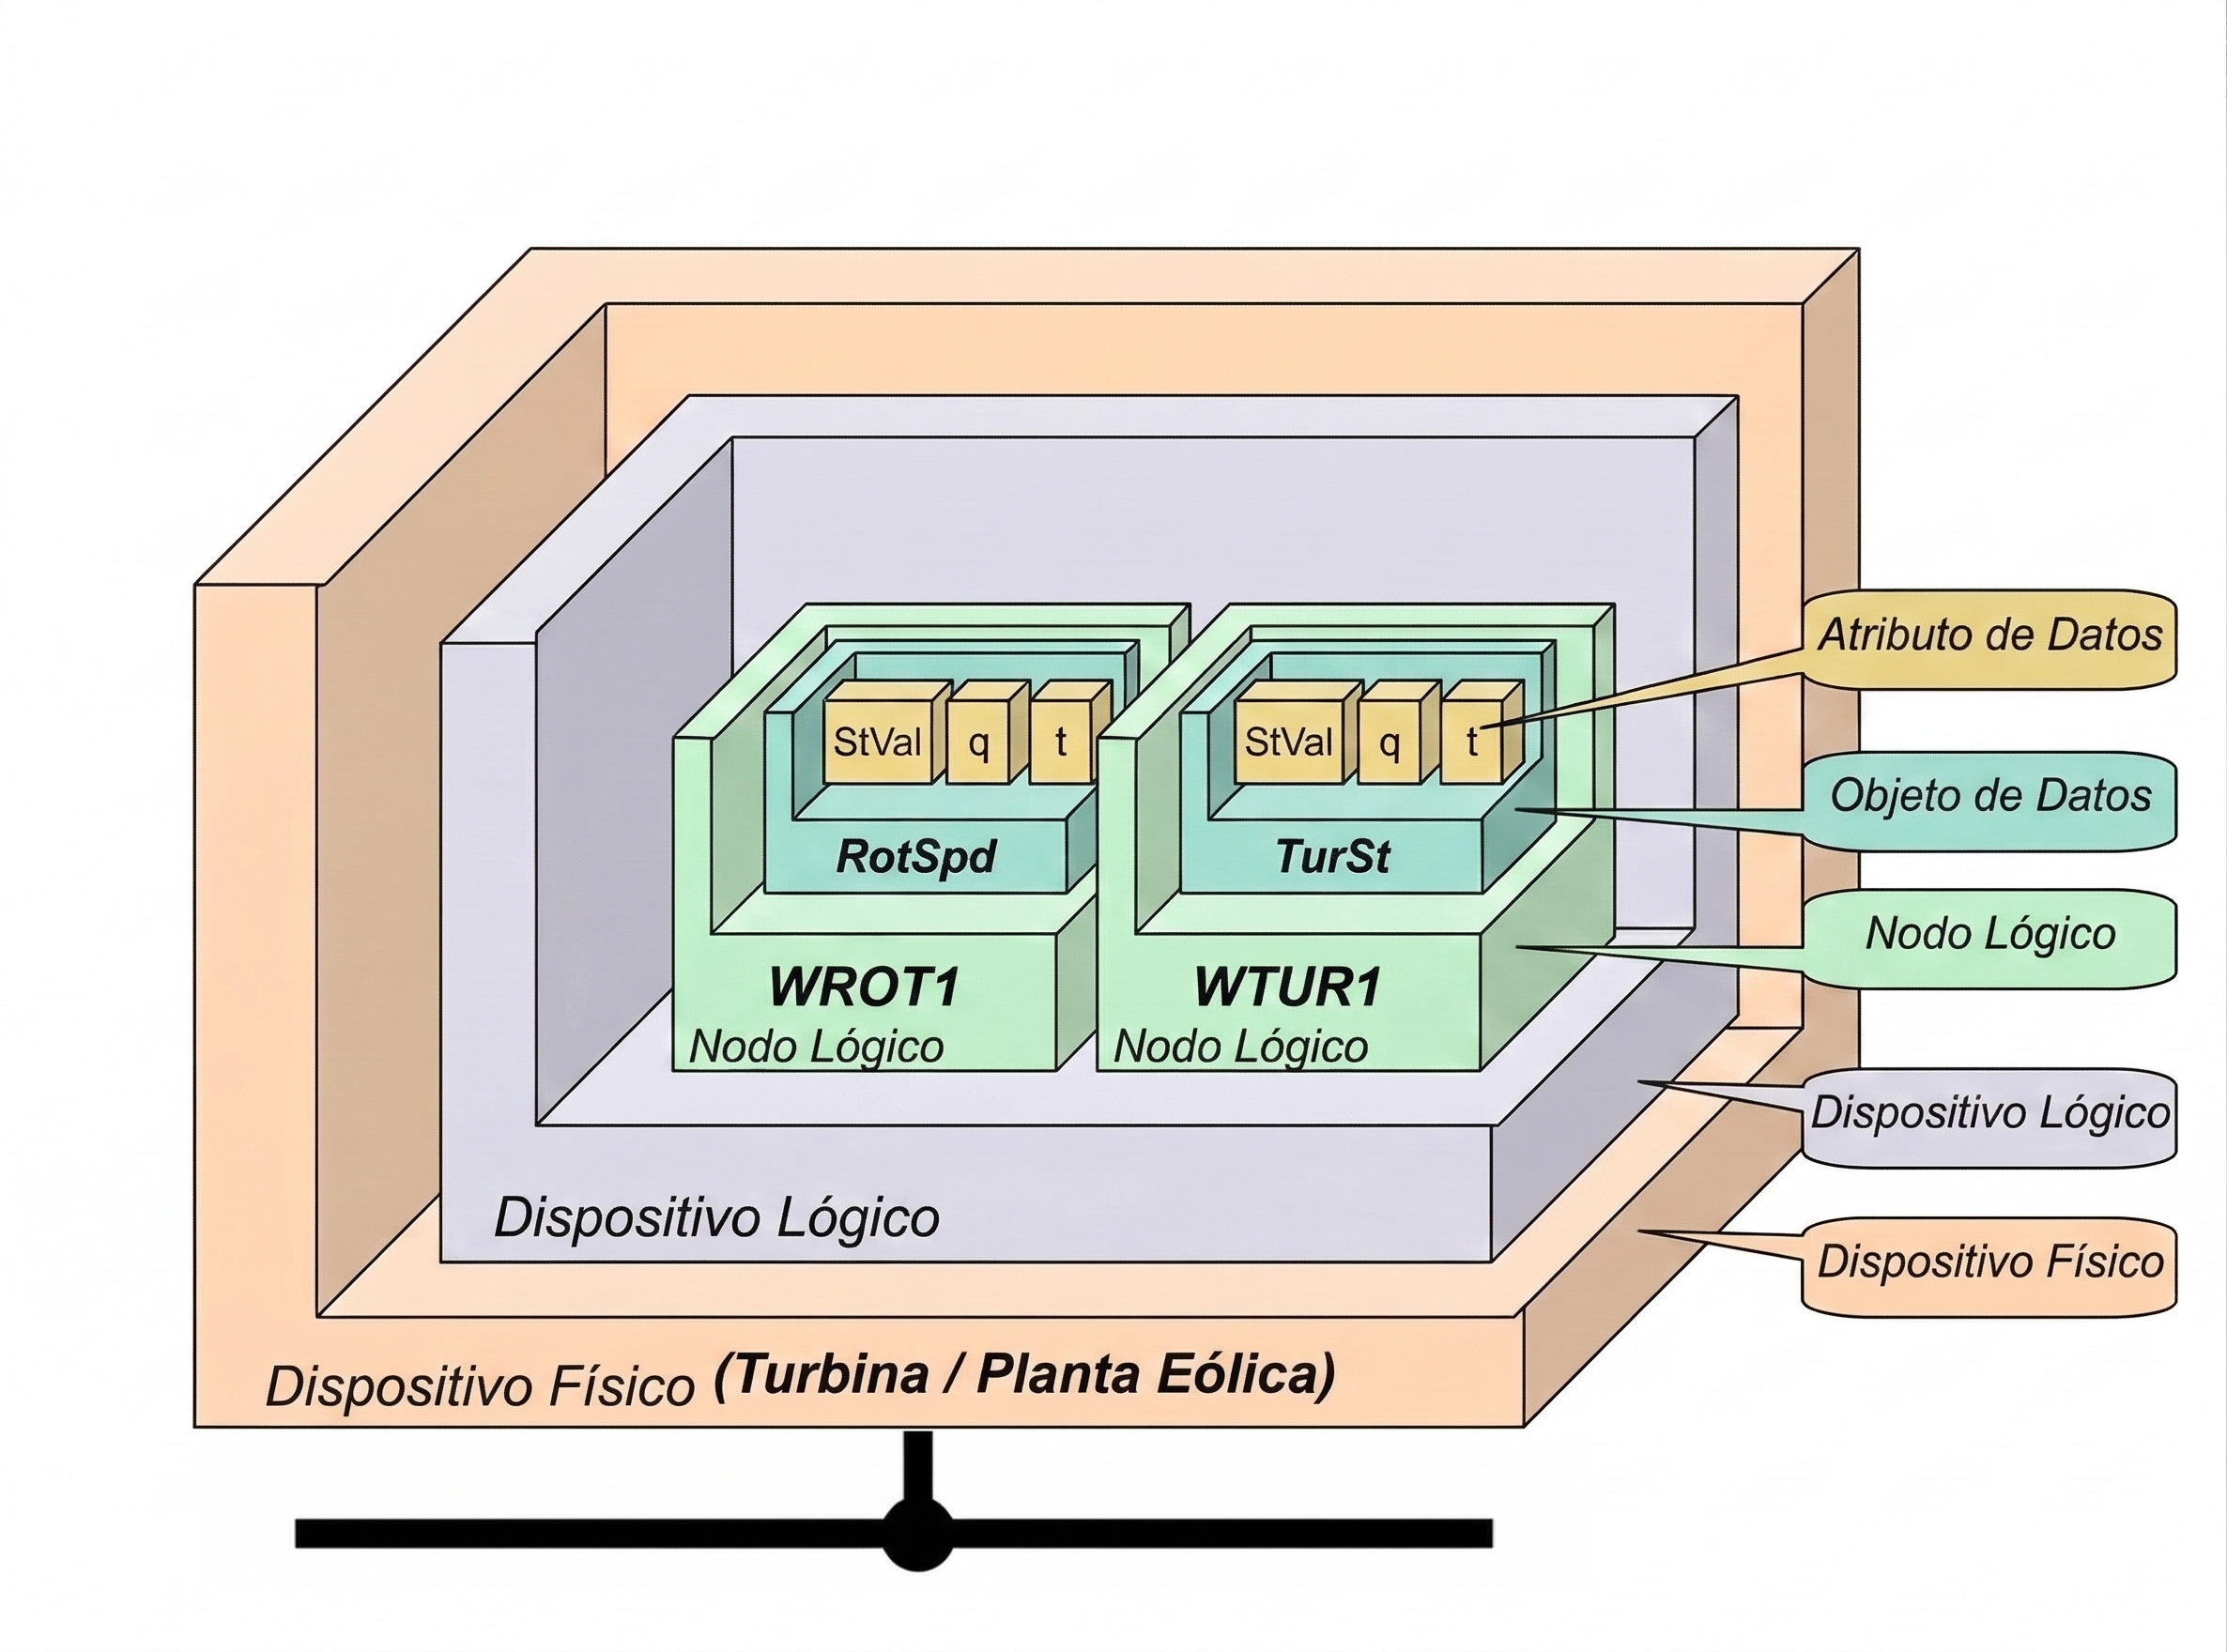
\includegraphics[scale=0.18]{figuras/Nodos.png}
    \caption{Jerarquía de los niveles de la norma IEC 61400-25-2. fuente: }
    \label{fig:Nodos}
\end{figure}
\begin{figure}[t]
    \centering
    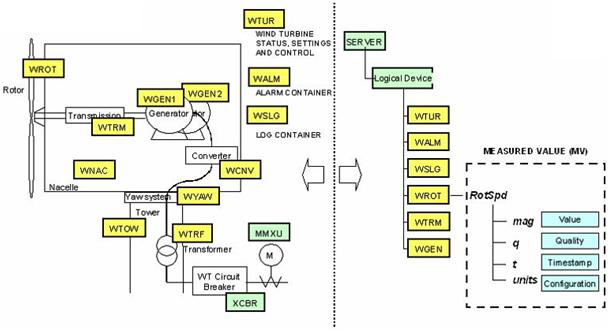
\includegraphics[scale=0.9]{figuras/IEC_61400-25-2_v1.jpg}
    \caption{Jerarquía de los niveles de la norma IEC 61400-25-2. fuente: https://www.iec.ch/standards/61400-25-2}
    \label{fig:IEC}
\end{figure}
\paragraph{Nivel 4: Atributos de Dato}
Se han diseñado las estructuras de variables de nivel 4 según la norma IEC 61400-25-2. En ellas se detallan las Clases de Datos Comunes (CDC), las cuales son utilizadas para representar los diferentes tipos de datos en el sistema segun el estándar. De esta forma se crea una base comun facilmente interpretable por cualquier sistema que siga la norma IEC 61400-25-2, lo que facilita la interoperabilidad entre diferentes dispositivos y sistemas dentro de un parque eólico. Las CDC definen la estructura y el formato de los datos, asegurando que la información se transmita de manera consistente y comprensible entre los componentes del sistema eólico. (Tabla \ref{tab:estructuras_nivel4})

\begin{table}[t]
    \centering
    \caption{Estructuras de variables de nivel 4 según norma IEC 61400-25-2.}
    \begin{tabular}{p{4cm} p{1cm} p{2.7cm} p{5cm}}
        
        \toprule
        \multicolumn{4}{c}{\textbf{Estructuras de Variables de nivel 4}} \\
        \midrule
        Nombre & Dato & Tipo de Dato & Descripción\\
        \midrule
        \multirow{3}{*}{\shortstack[l]{\textit{Single Point Status}\\ (SPS)}} & \textit{stVal} & Booleano & Valor de la variable\\
         & \textit{q} & Booleano & Calidad de la señal\\
         & \textit{t} & Timestamp & Tiempo de actualización\\
        
         \midrule
         \multirow{3}{*}{\shortstack[l]{\textit{Integer Status}\\ (INS)}} & \textit{stVal} & Entero con Signo de 16 bits & Valor de la variable\\
         & \textit{q} & Booleano & Calidad de la señal\\
         & \textit{t} & Timestamp & Tiempo de actualización\\
              
         \midrule
         \multirow{3}{*}{\shortstack[l]{\textit{Measured Value}\vspace{0.5cm} \\(MV)}} & \textit{mag} & Coma flotante IEEE 754 32bits & Valor de la variable\\
         & \textit{q} & Booleano & Calidad de la señal\\
         & \textit{t} & Timestamp & Tiempo de actualización\\
         
         \midrule
         \multirow{2}{*}{\shortstack[l]{\textit{Object ID} \\(ZID)}} & \textit{setVal} & Juego de caracteres ASCII & Valor de identificación del objeto \\
         & \textit{setSrc} & Entero sin signo de 16 bits & Identidad numérica\\
         
    
         \bottomrule
         
    \end{tabular}
    \vspace{0.5cm}
    \label{tab:estructuras_nivel4}
\end{table}

\paragraph{Nivel 2: Estructura de Nodos Lógicos (LN)}
La norma IEC 61400-25 define una jerarquía semántica donde el nivel 2 se identifica mediante siglas de tres o cuatro letras mayúsculas siendo la primera letra la que indica el tipo de objeto (Por ejemplo W para la turbina) seguido por letras que indican la función o característica específica del objeto (por ejemplo, ROT para objetos relacionados con la rotación de la turbina). Los nodos lógicos se agrupan por subsistemas, cada uno de ellos representando un área funcional específica dentro del parque eólico. Los nodos lógicos más relevantes en el contexto de un parque eólico son los siguientes:
\begin{itemize}
    \item \textbf{WGEN (Generator):} Agrupa toda la información relativa a la conversión electromecánica.
    \item \textbf{WROT (Rotor):} Contiene las variables cinemáticas del conjunto de palas y buje.
    \item \textbf{WYAW (Yaw System):} Gestiona los datos del sistema de orientación de la góndola.
    \item \textbf{WTRF (Transformer):} Supervisa el estado de los activos de transformación eléctrica.
\end{itemize}

Además, el estandar IEC 61400-25-2 viene heredado de la norma IEC 61850-7-4, la cual se desarrolló para la automatización de subestaciones eléctricas. Por lo tanto, el diseño de las estructuras de variables de nivel 2 deben incorporar atributos heredados de IEC 61850-7-4. Esos atributos heredados son los siguientes:

\begin{itemize}
    \item \textbf{\textit{Mod} (Modo):} Define el modo de operación deseado para el nodo lógico (Ej. On, Off, Auto, Manual, Test, etc.)
    \item \textbf{\textit{Beh} (Comportamiento):} Define el comportamiento del real del nodo lógico
    \item \textbf{\textit{Health} (Salud):} Define el estado de salud del nodo lógico
    \item \textbf{\textit{Loc} (Localización):} Define la ubicación física del nodo lógico
\end{itemize}


\paragraph{Nivel 3: Objetos de Datos y Variables de Proceso}
Finalmente, el Nivel 3 identifica las señales específicas que pueblan cada Nodo Lógico. Es en este punto donde la estructura toma su forma definitiva para el operador. Una variable de Nivel 3 (Data Object) adquiere su significado completo solo cuando se instancia dentro de un nodo y bajo una CDC específica.

En el entorno de desarrollo de SIMATIC WinCC V8.1, esta jerarquía se traduce en nombres de variables estructuradas con el formato \texttt{Nodo.Variable.CDC}. Para ilustrar esta integración final, la Tabla \ref{tab:ejemplo_jerarquia_ascendente} muestra cómo los niveles previamente explicados convergen para formar las etiquetas de proceso que utiliza el SCADA.

\begin{table}[t]
    \centering
    \caption{Ejemplo de construcción de señales mediante el enfoque ascendente.}
    \label{tab:ejemplo_jerarquia_ascendente}
    \begin{tabular}{@{}llll@{}}
        \toprule
        \textbf{Base (Nivel 4)} & \textbf{Contenedor (Nivel 2)} & \textbf{Variable (Nivel 3)} & \textbf{Tag Final en WinCC} \\ \midrule
        CDC: MV & LN: WGEN & DO: Spd & \texttt{WGEN.Spd.mag} \\
        CDC: MV & LN: WROT & DO: RotSpd & \texttt{WROT.RotSpd.mag} \\
        CDC: INS & LN: WMET & DO: WndSpd & \texttt{WMET.WndSpd.mag} \\
        CDC: INS & LN: WNAC & DO: Stop & \texttt{WNAC.YawSt.stVal} \\ \bottomrule
    \end{tabular}
\end{table}

\textit{Nota: El desglose exhaustivo de todos los Nodos Lógicos y sus correspondientes variables de Nivel 3, agrupados por subsistemas, se encuentra disponible para su consulta en el \textbf{Anexo I}.}
\section{Interfaz Gráfica}

La interfaz gráfica constituye el punto de interacción principal entre el operador y el sistema SCADA, por lo que su diseño debe priorizar la claridad, la rapidez de interpretación y la operabilidad en tiempo real. En esta sección se describe la propuesta de visualización desarrollada en WinCC, explicando la organización general de la interfaz y los criterios utilizados para su construcción.\par

Aunque en el diseño actual de interfaces industriales existe una fuerte tendencia hacia la adopción del estándar ISA-101 (High-Performance HMI) —que aboga por el uso casi exclusivo de escalas de grises, gráficos vectoriales abstractos y la minimización radical del color—, en el presente Trabajo Fin de Máster se ha decidido no aplicar este estándar de forma estricta por  razones técnicas y de alcance.\par

Por un lado, destaca el enfoque didáctico y demostrativo de esta prueba de concepto. Al abarcar desde la adquisición de datos de campo hasta la integración IIoT en la nube (AWS), una representación ilustrativa y a color facilita enormemente la comprensión inmediata del estado de los aerogeneradores durante la exposición del proyecto.\par

Por otro lado, se ha priorizado la optimización de recursos y la compatibilidad nativa empleando la \textit{Siemens Industry Graphic Library}. El aprovechamiento de estas paletas de color y controles predefinidos en WinCC V8.1 reduce los tiempos de diseño de la interfaz, permitiendo centrar los esfuerzos en arquitecturas más complejas como la comunicación OPC UA.

Por último, dada la potencia del software de desarrollo SIMATIC WinCC V8.1, se ha optado por una representación que aproveche al maximo las capacidades gráficas del entorno, demostrando así la capacidad de la plataforma para crear interfaces visualmente atractivas y funcionales, sin comprometer la claridad ni la operatividad. En definitiva, a pesar de no sustentarse estrictamente en el estandar ISA-101, la propuesta se ha diseñado con criterios de usabilidad y eficacia.


\subsection{Jerarquía de pantallas}
En concreto, se presenta la jerarquía de pantallas definida para la navegación (desde vistas generales hasta vistas de detalle), la estructura de menús y accesos, la distribución de los elementos de supervisión y las pautas de representación de estados, alarmas y variables de proceso. Con ello se justifica cómo la arquitectura gráfica facilita tanto la monitorización continua como la operación segura del sistema.

Para garantizar la escalabilidad, el mantenimiento y la correcta integración de la navegación dentro del entorno de desarrollo SIMATIC WinCC V8.1, se ha implementado un sistema de nomenclatura estandarizado para todos los archivos gráficos de la interfaz (\texttt{.pdl}). Este sistema adopta una estructura jerárquica y funcional, resultando indispensable para la gestión eficiente de proyectos de automatización con un alto volumen de variables y pantallas.

El patrón de diseño definido para nombrar cada interfaz se fundamenta en tres bloques lógicos: \texttt{[Nivel]\_[Categoría]\_[Descripción\_Funcional]} (figura \ref{fig:jerarquia_pantallas}).
\begin{figure}[t]
    \centering
    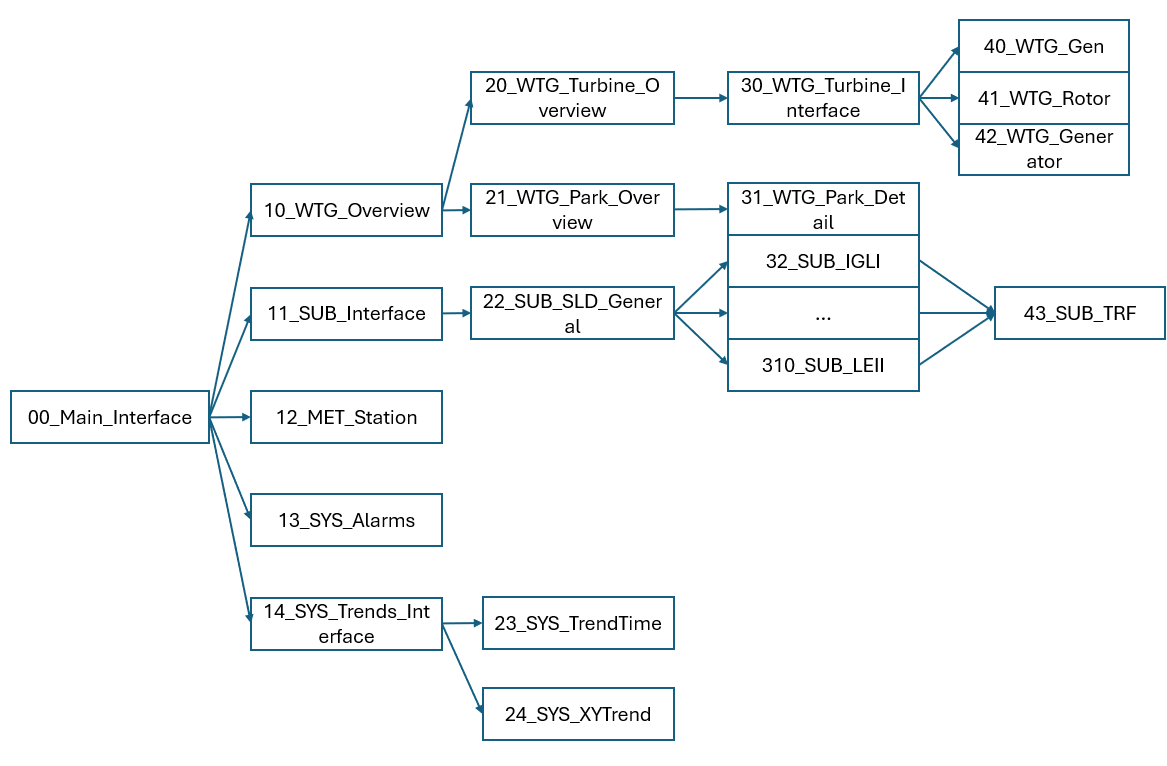
\includegraphics[scale=0.45]{figuras/jerarquia.png}
    \caption{Ejemplo de jerarquía de pantallas en una interfaz gráfica de supervisión industrial.}
    \label{fig:jerarquia_pantallas}
\end{figure}
\subsubsection{Prefijo Numérico (Jerarquía y Orden de Navegación)}
El primer bloque numérico determina la profundidad de la pantalla dentro del árbol de navegación del SCADA, marcando el flujo operativo:
\begin{itemize}
    \item \textbf{00 (Nivel Raíz):} Reservado exclusivamente para el marco base de la aplicación y la pantalla de inicio principal (\texttt{00\_Main\_Interface}).Físicamente, la arquitectura gráfica se sustenta en esta plantilla maestra que actúa como \textbf{Nivel 0} o marco base.(figura \ref{fig:interfaz_grafica}).
    \item \textbf{1X (Áreas Principales):} Define las divisiones macroscópicas del parque eólico. Incluye la vista general de los aerogeneradores (\texttt{10}), la subestación eléctrica (\texttt{11}), la estación meteorológica (\texttt{12}) y los servicios de diagnóstico del sistema (\texttt{13}, \texttt{14}).
    \item \textbf{2X, 3X, 4X (Niveles de Detalle y Equipos):} Representan submenús y el desglose técnico de los activos. A medida que se incrementa el dígito inicial, aumenta el detalle de la información supervisada. Por ejemplo, los niveles 40, 41 y 42 se destinan a la monitorización de subsistemas de los aerogeneradores, como el generador o el rotor.
    \item \textbf{9X (Pop Ups y Faceplates):} Se reservan para pantallas de uso específico, como ventanas emergentes de alarmas, plantillas de variables (\textit{Faceplates}) o interfaces de configuración avanzada. Estas pantallas no forman parte del flujo de navegación principal, sino que se activan bajo demanda para tareas puntuales.
\end{itemize}

\subsubsection{Identificador de Categoría (Clasificación de Activos)}
El segundo bloque emplea acrónimos técnicos para identificar de forma unívoca la familia de sistemas a la que pertenece la interfaz:
\begin{itemize}
    \item \textbf{WTG (Wind Turbine Generator):} Pantallas dedicadas a la monitorización, control y operación directa de los aerogeneradores.
    \item \textbf{SUB (Substation):} Interfaz enfocada en la infraestructura eléctrica de evacuación, esquemas unifilares y transformadores.
    \item \textbf{MET (Meteorological):} Visualización de los datos climáticos adquiridos por la torre meteorológica.
    \item \textbf{SYS (System):} Funcionalidades globales del entorno SCADA, abarcando la gestión de alarmas y las pantallas de tendencias (\textit{Trends}).
\end{itemize}

\subsubsection{Descripción Funcional}
El tercer bloque explicita el propósito operativo de la pantalla, agilizando su localización por parte del programador o integrador:
\begin{itemize}
    \item \textbf{Overview:} Vista panorámica que agrega los indicadores clave (KPIs) y el estado general de un conjunto de activos.
    \item \textbf{Interface / Detail:} Panel de control principal o plantilla (\textit{Faceplate}) que detalla las variables operativas de un equipo.
    \item \textbf{SLD (Single Line Diagram):} Representación dinámica del esquema eléctrico unifilar.
    \item \textbf{Gen / Rotor / TRF:} Identificadores concretos de subsistemas electromecánicos (Generador, Rotor, Transformador).
\end{itemize}

\vspace{0.5cm}
La adopción de esta nomenclatura trasciende la mera organización de archivos; define la lógica de navegación \textit{Top-Down} requerida en la operación de plantas de generación. El operador inicia la supervisión en una vista global (\texttt{10\_WTG\_Overview}), focaliza la atención en una turbina particular (\texttt{30\_WTG\_Turbine\_Interface}) y profundiza en el diagnóstico de sus componentes mecánicos (\texttt{40\_WTG\_Gen}).\par 

Asimismo, esta estandarización resulta determinante para optimizar el rendimiento de la aplicación gráfica. Al mantener nombres predecibles y estructurados, se facilita el uso de \textit{scripts} y ventanas de imagen (\textit{Picture Windows}) dinámicas, permitiendo que una única pantalla genérica actúe como interfaz para cualquier aerogenerador del parque mediante el paso de parámetros y prefijos de variables estructuradas (\textit{Tag Prefixes}).\par

Para mantener esta filosofía, la navegación del sistema se ha estructurado implementando un diseño centralizado basado en estas ventanas de imagen. Esta técnica de SIMATIC WinCC permite mantener un marco estático de control mientras el área de trabajo cambia dinámicamente. La base física de esta jerarquía se fundamenta en el siguiente elemento:\par

\subsection{Nivel 0: Marco Base (\texttt{00\_Main\_Interface})}
Representa la interfaz matriz o \textbf{Nivel 0} del SCADA (véase Figura \ref{fig:interfaz_grafica}). En lugar de ejecutar transiciones de pantalla completa, esta plantilla actúa como un contenedor estático  que alberga el menú de navegación principal e implementa dos \textit{Picture Windows} independientes.\par

La \textbf{ventana de trabajo central} ocupa la mayor parte de la pantalla y constituye el área de visualización dinámica donde se cargan todas las interfaces operativas (Niveles 1 a 4). Paralelamente, la \textbf{ventana de alarmas inferior} es un espacio de menores dimensiones anclado de forma fija en el pie de página, cuya única función es garantizar la supervisión ininterrumpida de los eventos críticos independientemente de la profundidad de navegación del usuario.

\begin{figure}[t]
    \centering
    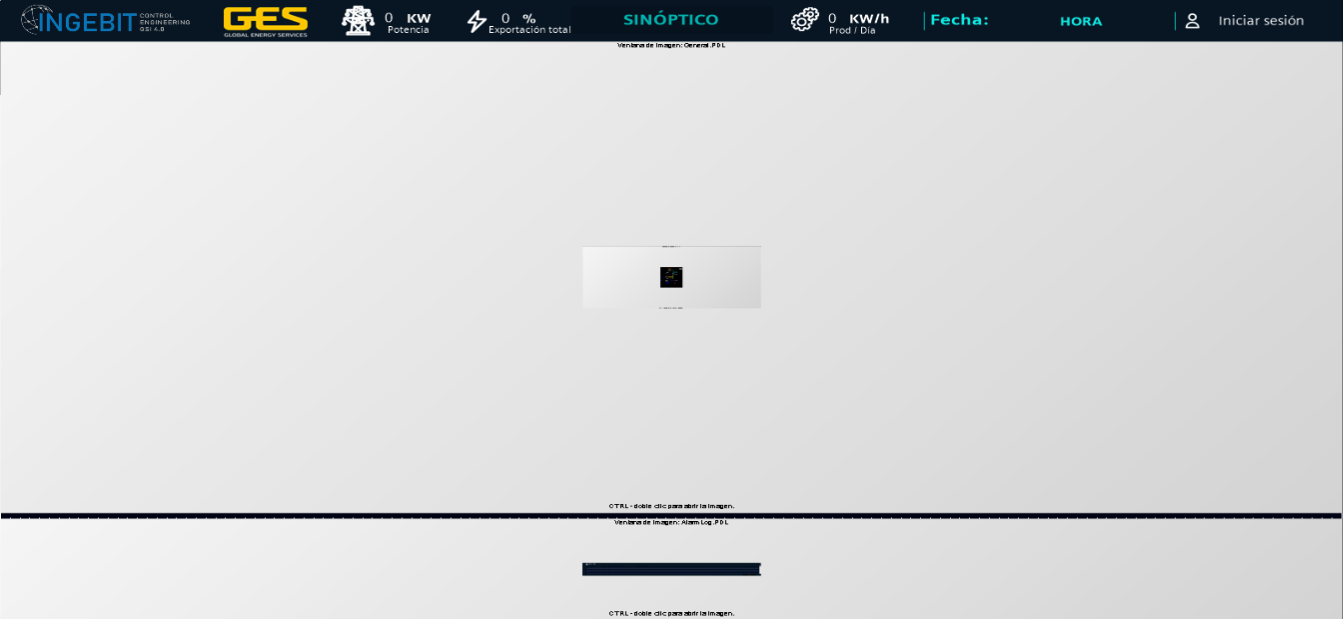
\includegraphics[scale=0.4]{figuras/GUI.png}
    \caption{Ejemplo de interfaz gráfica desarrollada en WinCC para la supervisión de un proceso industrial.}
    \label{fig:interfaz_grafica}
\end{figure}
\FloatBarrier
\subsection{Nivel 1: Supervisión Global}
\label{sec:nivel_1_overview}
\subsubsection{Vista General de aerogeneradores (\texttt{10\_WTG\_Overview})}
La pantalla \texttt{10\_WTG\_Overview} actúa como el nodo principal de enrutamiento dinámico del SCADA. Su diseño optimiza la navegación hacia los niveles inferiores mediante tres mecanismos clave integrados en su cabecera.

Por un lado, se ha implementado un sistema de filtrado mediante dos selectores desplegables (Estado y Subestación) que acotan la información visualizada, actualizando los aerogeneradores mostrados sin necesidad de realizar transiciones a otras pantallas ( Algoritmo \ref{alg:filtrado_dinamico}, vease la función \texttt{AplicarFiltroPosicion()} en el Anexo \ref{cap:anexo_codigo_solucion}).\par

Por otro lado, un selector central gestiona el archivo alojado en el \textit{Picture Window} de trabajo. Permite alternar instantáneamente entre la telemetría individual de las máquinas (\texttt{20\_WTG\_Turbine\_Overview.pdl}) y la vista de datos por parques (\texttt{21\_WTG\_Park\_Overview.pdl}).\par

Finalmente, una matriz superior de indicadores discretos organizados por parques representa el estado de cada aerogenerador. Seleccionar uno de ellos actúa como acceso directo al Nivel 4 (\texttt{40\_WTG\_Gen}), omitiendo pasos intermedios e inyectando automáticamente el \textit{Tag Prefix} correspondiente para cargar los datos de la máquina seleccionada.\par

\begin{figure}[t]
    \centering
    % Ajusta la ruta de tu imagen
    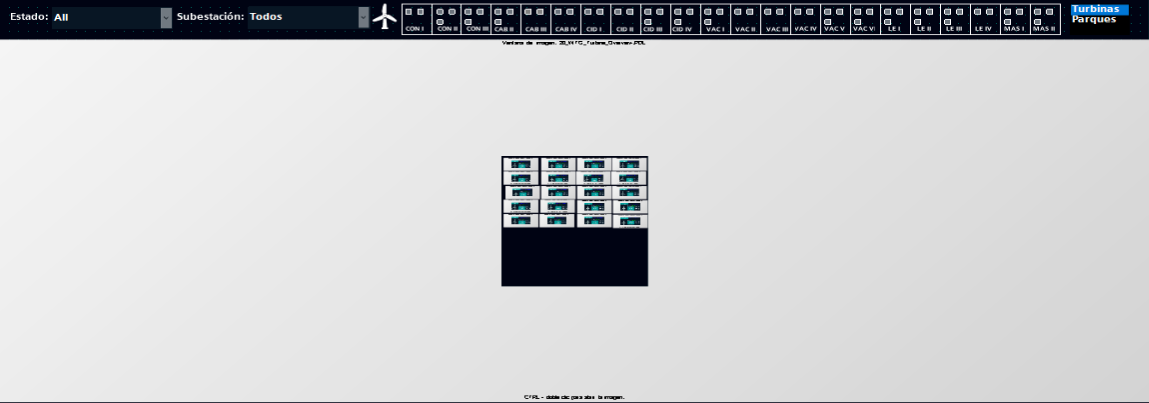
\includegraphics[width=\textwidth]{figuras/10_WTG_Overview.png}
    \caption{Cabecera de navegación en \texttt{10\_WTG\_Overview}, mostrando filtros, selector de vista y matriz de accesos directos.}
    \label{fig:10_wtg_overview}
\end{figure}


\FloatBarrier
\subsubsection{Intefaz de diagrama electrico (\texttt{11\_SUB\_Interface})}
\label{sec:nivel_1_subestacion}
Esta pantalla actúa como un contenedor especializado para la visualización de la infraestructura eléctrica del parque. Arquitectónicamente, se ha diseñado como una interfaz intermedia que alberga un único \textit{Picture Window} destinado a cargar los diversos diagramas unifilares (\textit{Single Line Diagrams}).\par

La decisión de no integrar estos esquemas directamente en la pantalla raíz (\texttt{00\_Main\_Interface}) y emplear este encapsulamiento responde a dos criterios técnicos fundamentales, por un lado, la gestión de la visualización y desplazamiento de diagramas eléctricos complejos (\textit{scrolling}), y por otro, el aislamiento de variables mediante \textit{Tag Prefixes} para evitar interferencias con el entorno principal del SCADA.\par

\begin{figure}[t]
    \centering
    % Ajusta la ruta de tu imagen cuando la tengas
    
\includegraphics[width=\textwidth]{figuras/11_SUB_Interfaec.png}
    \caption{Estructura de contenedor para esquemas eléctricos en \texttt{11\_SUB\_Interface}.}
    \label{fig:11_sub_interface}
\end{figure}

\FloatBarrier
\subsection{Nivel 9: Plantillas dinámicas y reutilización gráfica (\textit{Tag Prefix})}
\label{sec:tag_prefix}

En la monitorización de parques eólicos, la topología del sistema presenta una alta repetición de activos físicos idénticos (decenas de aerogeneradores con la misma instrumentación). Desarrollar un archivo \texttt{.pdl} individual para cada turbina o clúster resultaría ineficiente, consumiendo recursos excesivos del sistema y dificultando el mantenimiento futuro del SCADA. 

Para resolver esta problemática, el diseño de las interfaces de detalle se ha fundamentado en el principio de reutilización gráfica, combinando el uso de las variables de estructura (definidas en el apartado 7.4.3) con la propiedad \textit{Tag Prefix} (Prefijo de variable) de las ventanas de imagen (\textit{Picture Windows}) de SIMATIC WinCC.

La técnica consiste en diseñar una única pantalla genérica (\textit{Faceplate} maestro) donde los objetos gráficos (barras, campos de texto, indicadores de estado) se vinculan a las variables sin especificar la turbina a la que pertenecen (por ejemplo, apuntando a la variable \texttt{.WROT.RotAzi.mag} en lugar de \texttt{WTG1.WROT.RotAzi.mag}).

Durante la operación en el entorno \textit{Runtime}, cuando el operador selecciona un aerogenerador específico desde la vista general, se ejecuta un \textit{script} que realiza dos acciones simultáneas sobre el \textit{Picture Window} central:
\begin{enumerate}
    \item Carga el archivo \texttt{.pdl} de la plantilla genérica.
    \item Asigna el nombre de la turbina seleccionada (ej. \texttt{WTG1}) a la propiedad \textit{Tag Prefix} de la ventana.
\end{enumerate}

Automáticamente, WinCC concatena este prefijo con el sufijo interno de los objetos gráficos, dinamizando la pantalla completa con los datos reales del equipo seleccionado en cuestión de milisegundos. Esta filosofía se ha aplicado intensivamente en los niveles principales del proyecto

\paragraph{Vistas de detalle de Turbina (\textit{Turbine Overview})}
Estas interfaces proporcionan la telemetría resumida de un único aerogenerador. Como se observa en la Figura \ref{fig:overview_turbina}, la pantalla despliega de forma concisa los valores críticos (velocidad del viento local, régimen del rotor, estado del \textit{pitch} y temperaturas clave). Gracias al \textit{Tag Prefix}, esta misma disposición gráfica sirve para supervisar cualquier máquina del parque eólico.

\begin{figure}[t]
    \centering
    \begin{minipage}[t]{0.45\textwidth}
        \centering
        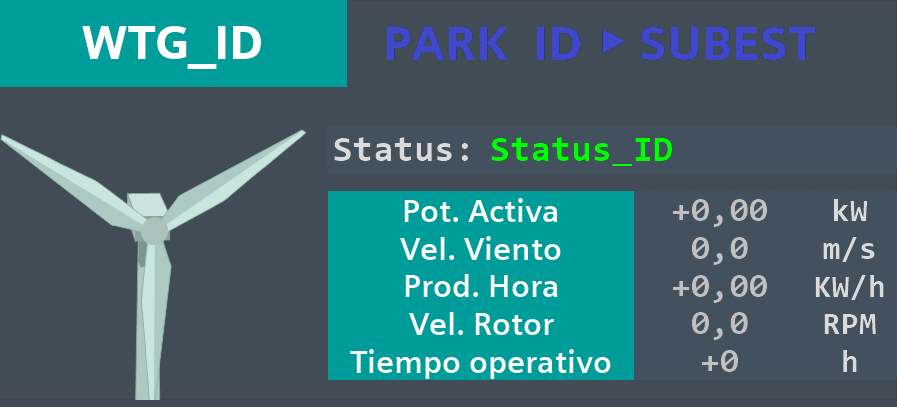
\includegraphics[width=\textwidth]{figuras/WTG_Faceplate.png}
        \caption{Plantilla genérica de monitorización de turbina, dinamizada mediante \textit{Tag Prefix}.}
        \label{fig:overview_turbina}
    \end{minipage}
    \hfill
    \begin{minipage}[t]{0.45\textwidth}
        \centering
        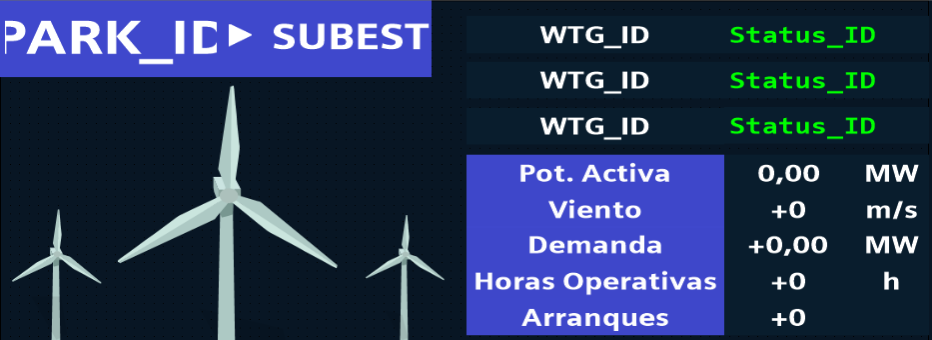
\includegraphics[width=\textwidth]{figuras/Park_Faceplate.png}
        \caption{Pantalla de supervisión de clúster/parque, empleando variables estructuradas para la agregación de datos.}
        \label{fig:overview_parque}
    \end{minipage}
\end{figure}
\paragraph{Vistas de agrupación o clústeres (\textit{Park Overview})}
De manera análoga a las turbinas individuales, el parque puede subdividirse en subestaciones o clústeres lógicos. Se ha diseñado una plantilla de agrupación que, recibiendo el prefijo correspondiente al clúster, consolida y visualiza los datos agregados de un subconjunto de aerogeneradores (Figura \ref{fig:overview_parque}), optimizando drásticamente el número de archivos en el proyecto y garantizando la homogeneidad visual de la interfaz.


\FloatBarrier
\subsection{Scripts globales}





\begin{algorithm}[t]
    
    \DontPrintSemicolon
    \SetKwFunction{FRead}{LeerTag}
    \SetKwFunction{FHide}{OcultarFaceplate}
    \SetKwFunction{FShow}{MostrarFaceplate}
    \SetKwFunction{FMove}{MoverFaceplate}
    \SetKwFunction{FMap}{MapearEstadoHMI}
    \vspace{1cm}
    Establecer cuadriculas, numero de molinos, prefijos de variables, offsets y posiciones iniciales \par

    Ocultar todos los faceplates de molinos como limpieza inicial \;

    \For{(Numero de molinos Do)}
    {
        \FHide{$i$} \;
    }
    Bucle de filtrado y posicionamiento \;
    \For{(Numero de molinos $i$ Do)}
    {
        $Estado \leftarrow \FRead{\text{Estado PLC Molino } i}$ \;
        $Parque \leftarrow \FRead{\text{ID Parque Molino } i}$ \;
        $Selector \leftarrow \FMap{Selector del HMI}$ \;

        \If{(si el selector es igual al parque del molino $i$ o esta en modo "todos")}
        {
            \FShow{$i$} \;
            \FMove{$i$} \;
            Siguiente columna\;
            \If{(superado el numero de columnas por fila)}
            {
                pasar a siguiente fila\;
            }
        }
    }
    \caption{Filtrado Dinámico y Posicionamiento de Aerogeneradores en Cuadrícula}
    \label{alg:filtrado_dinamico}
\end{algorithm}

\section{Gestión de alarmas y eventos}
\label{sec:alarmas}

La gestión de alarmas y eventos es el componente crítico del sistema SCADA encargado de garantizar la seguridad operativa y la conciencia situacional del operador. Su función principal no es solo la detección de anomalías, sino la jerarquización de las mismas para evitar la saturación de información durante incidentes críticos. 

En este proyecto, la supervisión de eventos se integra de forma transversal mediante el \textit{Picture Window} inferior persistente en la pantalla \texttt{00\_Main\_Interface}. Este diseño asegura que, independientemente del nivel de navegación en el que se encuentre el usuario, las notificaciones de mayor prioridad sean visibles de forma inmediata. La implementación se ha realizado empleando el objeto \textit{WinCC Alarm Control}, configurando ciclos de refresco en tiempo real y almacenamiento en una base de datos SQL histórica para auditorías posteriores.

\subsection{Criterios de señalización: Norma IEC 60073}

Para garantizar una interpretación unívoca de los estados del proceso, se ha seguido la normativa internacional \textbf{IEC 60073} (\textit{Principios básicos y de seguridad para las interfaces hombre-máquina, el marcado y la identificación}) \cite{iec60073}. Esta norma establece una codificación cromática estricta basada en el significado de la seguridad y el estado del equipo:

\begin{itemize}
    \item \textbf{Rojo:} Indica una situación de peligro, emergencia o actuación inmediata.
    \item \textbf{Amarillo/Ámbar:} Señala una condición anormal o un cambio crítico de estado que requiere precaución o supervisión.
    \item \textbf{Verde:} Representa una condición normal de funcionamiento o seguridad.
    \item \textbf{Azul:} Indica una condición de carácter obligatorio o una intervención específica del operador.
    \item \textbf{Blanco/Gris:} Utilizado para estados neutros o falta de información específica de seguridad.
\end{itemize}

\subsection{Codificación de estados de la turbina}

La determinación de los estados operativos del aerogenerador se fundamenta en el modelo de información de la norma \textbf{IEC 61400-25}, la cual define la turbina como una máquina de estados finitos. Sin embargo, dado que esta norma no especifica una paleta cromática para las interfaces gráficas (HMI), la representación visual se ha diseñado hibridando los principios de seguridad de la norma \textbf{IEC 60073} con los estándares \textit{de facto} aceptados en la industria de generación eólica.

El objetivo de esta asignación es garantizar que el operador comprenda la situación del parque en un solo vistazo, reservando los colores de alta saturación exclusivamente para condiciones que requieran atención. En la Tabla \ref{tab:colores_estados} se detalla la justificación técnica de la paleta adoptada:

\begin{table}[htbp]
    \centering
    \caption{Asignación de colores y estados de la turbina (Adaptación IEC 60073 a la industria eólica).}
    \label{tab:colores_estados}
    \begin{tabular}{@{}p{2.5cm}p{6cm}p{4cm}@{}}
        \toprule
        \textbf{Estado} & \textbf{Significado Operativo} & \textbf{Color HMI (IEC 60073)} \\ \midrule
        \texttt{Emergencia} & Parada por cadena de seguridad de hardware. & \textbf{Rojo} (Peligro) \\
        \texttt{Fallo} & Avería de software o componente. & \textbf{Rojo} (Alarma) \\
        \texttt{Mantenimiento} & Intervención técnica local (control remoto deshabilitado). & \textbf{Naranja / Amarillo} (Precaución / Advertencia) \\
        \texttt{Arrancando} & Fase de transición temporal (conexión a red). & \textbf{Azul} (Estado específico) \\
        \texttt{Apagando} & Fase de transición temporal (desconexión). & \textbf{Azul} (Estado específico) \\
        \texttt{Marcha} & Producción nominal conectada a red. & \textbf{Verde} (Condición normal/segura) \\
        \texttt{Pausa} & Standby por condiciones externas (ej. falta de viento). & \textbf{Blanco} (Condición neutra) \\
        \texttt{Parado} & Estado neutro, turbina desenergizada o parada manual. & \textbf{Gris} (Inactivo) \\ \bottomrule
    \end{tabular}
\end{table}

\textbf{Justificación del diseño cromático:}
\begin{itemize}
    \item \textbf{Uso del Azul:} Según la IEC 60073, el azul se emplea para estados que tienen un significado específico que no implica alarma ni normalidad absoluta. En el sector eólico, se ha estandarizado su uso para indicar estados de transición automatizados (\textit{Arrancando} y \textit{Apagando}), informando al operador de que la máquina está realizando una secuencia lógica sin necesidad de intervención humana.
    \item \textbf{Uso del Naranja/Amarillo:} Se asigna al modo \textit{Mantenimiento} para advertir a los operadores del centro de control que existen técnicos físicos trabajando en la turbina, funcionando como una alerta visual (equivalente a un \textit{Lockout/Tagout} virtual) que prohíbe el envío de comandos remotos.
    \item \textbf{Uso del Blanco y Gris:} Siguiendo los principios de HMI de alto rendimiento, los estados de \textit{Pausa} y \textit{Parada} (que son condiciones seguras y estacionarias) se representan en escala de grises. Esto reduce la fatiga visual del operador y evita que un parque sin viento parezca un panel de alarmas encendido.
\end{itemize}

\section{Integración de IIoT en la solución}

En el contexto actual de la Industria 4.0, la monitorización y supervisión de infraestructuras energéticas distribuidas, como es el caso de un parque eólico, se demandan soluciones que vayan más allá de los sistemas SCADA tradicionales aislados en planta. La convergencia entre las Tecnologías de la Operación (OT) y las Tecnologías de la Información (IT) permite habilitar el ecosistema del Internet Industrial de las Cosas (IIoT), facilitando el análisis de datos a gran escala, la accesibilidad remota y la escalabilidad del sistema.\par

Este capítulo describe en detalle el diseño, despliegue e integración de una arquitectura en la nube orientada a la adquisición y visualización de datos  provenientes de los aerogeneradores. Mientras que el sistema local (basado en SIMATIC WinCC V8.1) se encarga de la adquisición en tiempo real (Edge) y el control a nivel de campo mediante protocolos industriales como OPC UA, la arquitectura propuesta en este capítulo tiene como misión exportar estos datos de manera segura y eficiente hacia la nube para su almacenamiento histórico y explotación visual.\par

Para lograr un sistema robusto, modular y replicable, se ha diseñado una arquitectura basada en microservicios contenerizados, apoyada en las siguientes capas lógicas (figura \ref{fig:IIoT}):

\begin{itemize}
    \item Capa de Adquisición y Emisión (Edge): Representada por el módulo Cloud Connect del SCADA WinCC, encargado de empaquetar las variables de proceso (velocidad del viento, potencia generada, estados, etc.) y publicarlas mediante el protocolo de mensajería ligero MQTT.
    \item Capa de Infraestructura (Cloud): Soportada por una instancia virtual (EC2) alojada en Amazon Web Services (AWS), que proporciona el entorno computacional necesario con alta disponibilidad. El despliegue de los servicios se ha orquestado íntegramente mediante Docker, garantizando el aislamiento de los procesos y facilitando futuras migraciones.
    \item Capa de Ingesta y Procesamiento Intermedio: Implementada con Node-RED, que actúa como cliente MQTT para la suscripción a los tópicos de la planta, y proporciona un entorno de flujo de datos visual (flow-based programming) para filtrar, normalizar y transformar las tramas JSON recibidas antes de su inserción en la base de datos.
    \item Capa de Almacenamiento (TSDB): Soportada por InfluxDB, una base de datos de series temporales optimizada para la escritura de alta frecuencia y el almacenamiento eficiente de datos con marcas de tiempo (timestamps), características inherentes a la telemetría industrial.
    \item Capa de Visualización e Inteligencia de Negocio: Desarrollada sobre Grafana, que consulta directamente a la base de datos para construir dashboards interactivos, permitiendo la monitorización del rendimiento del parque eólico desde cualquier ubicación con acceso a internet.
\end{itemize}

\begin{figure}[t]
    \centering
    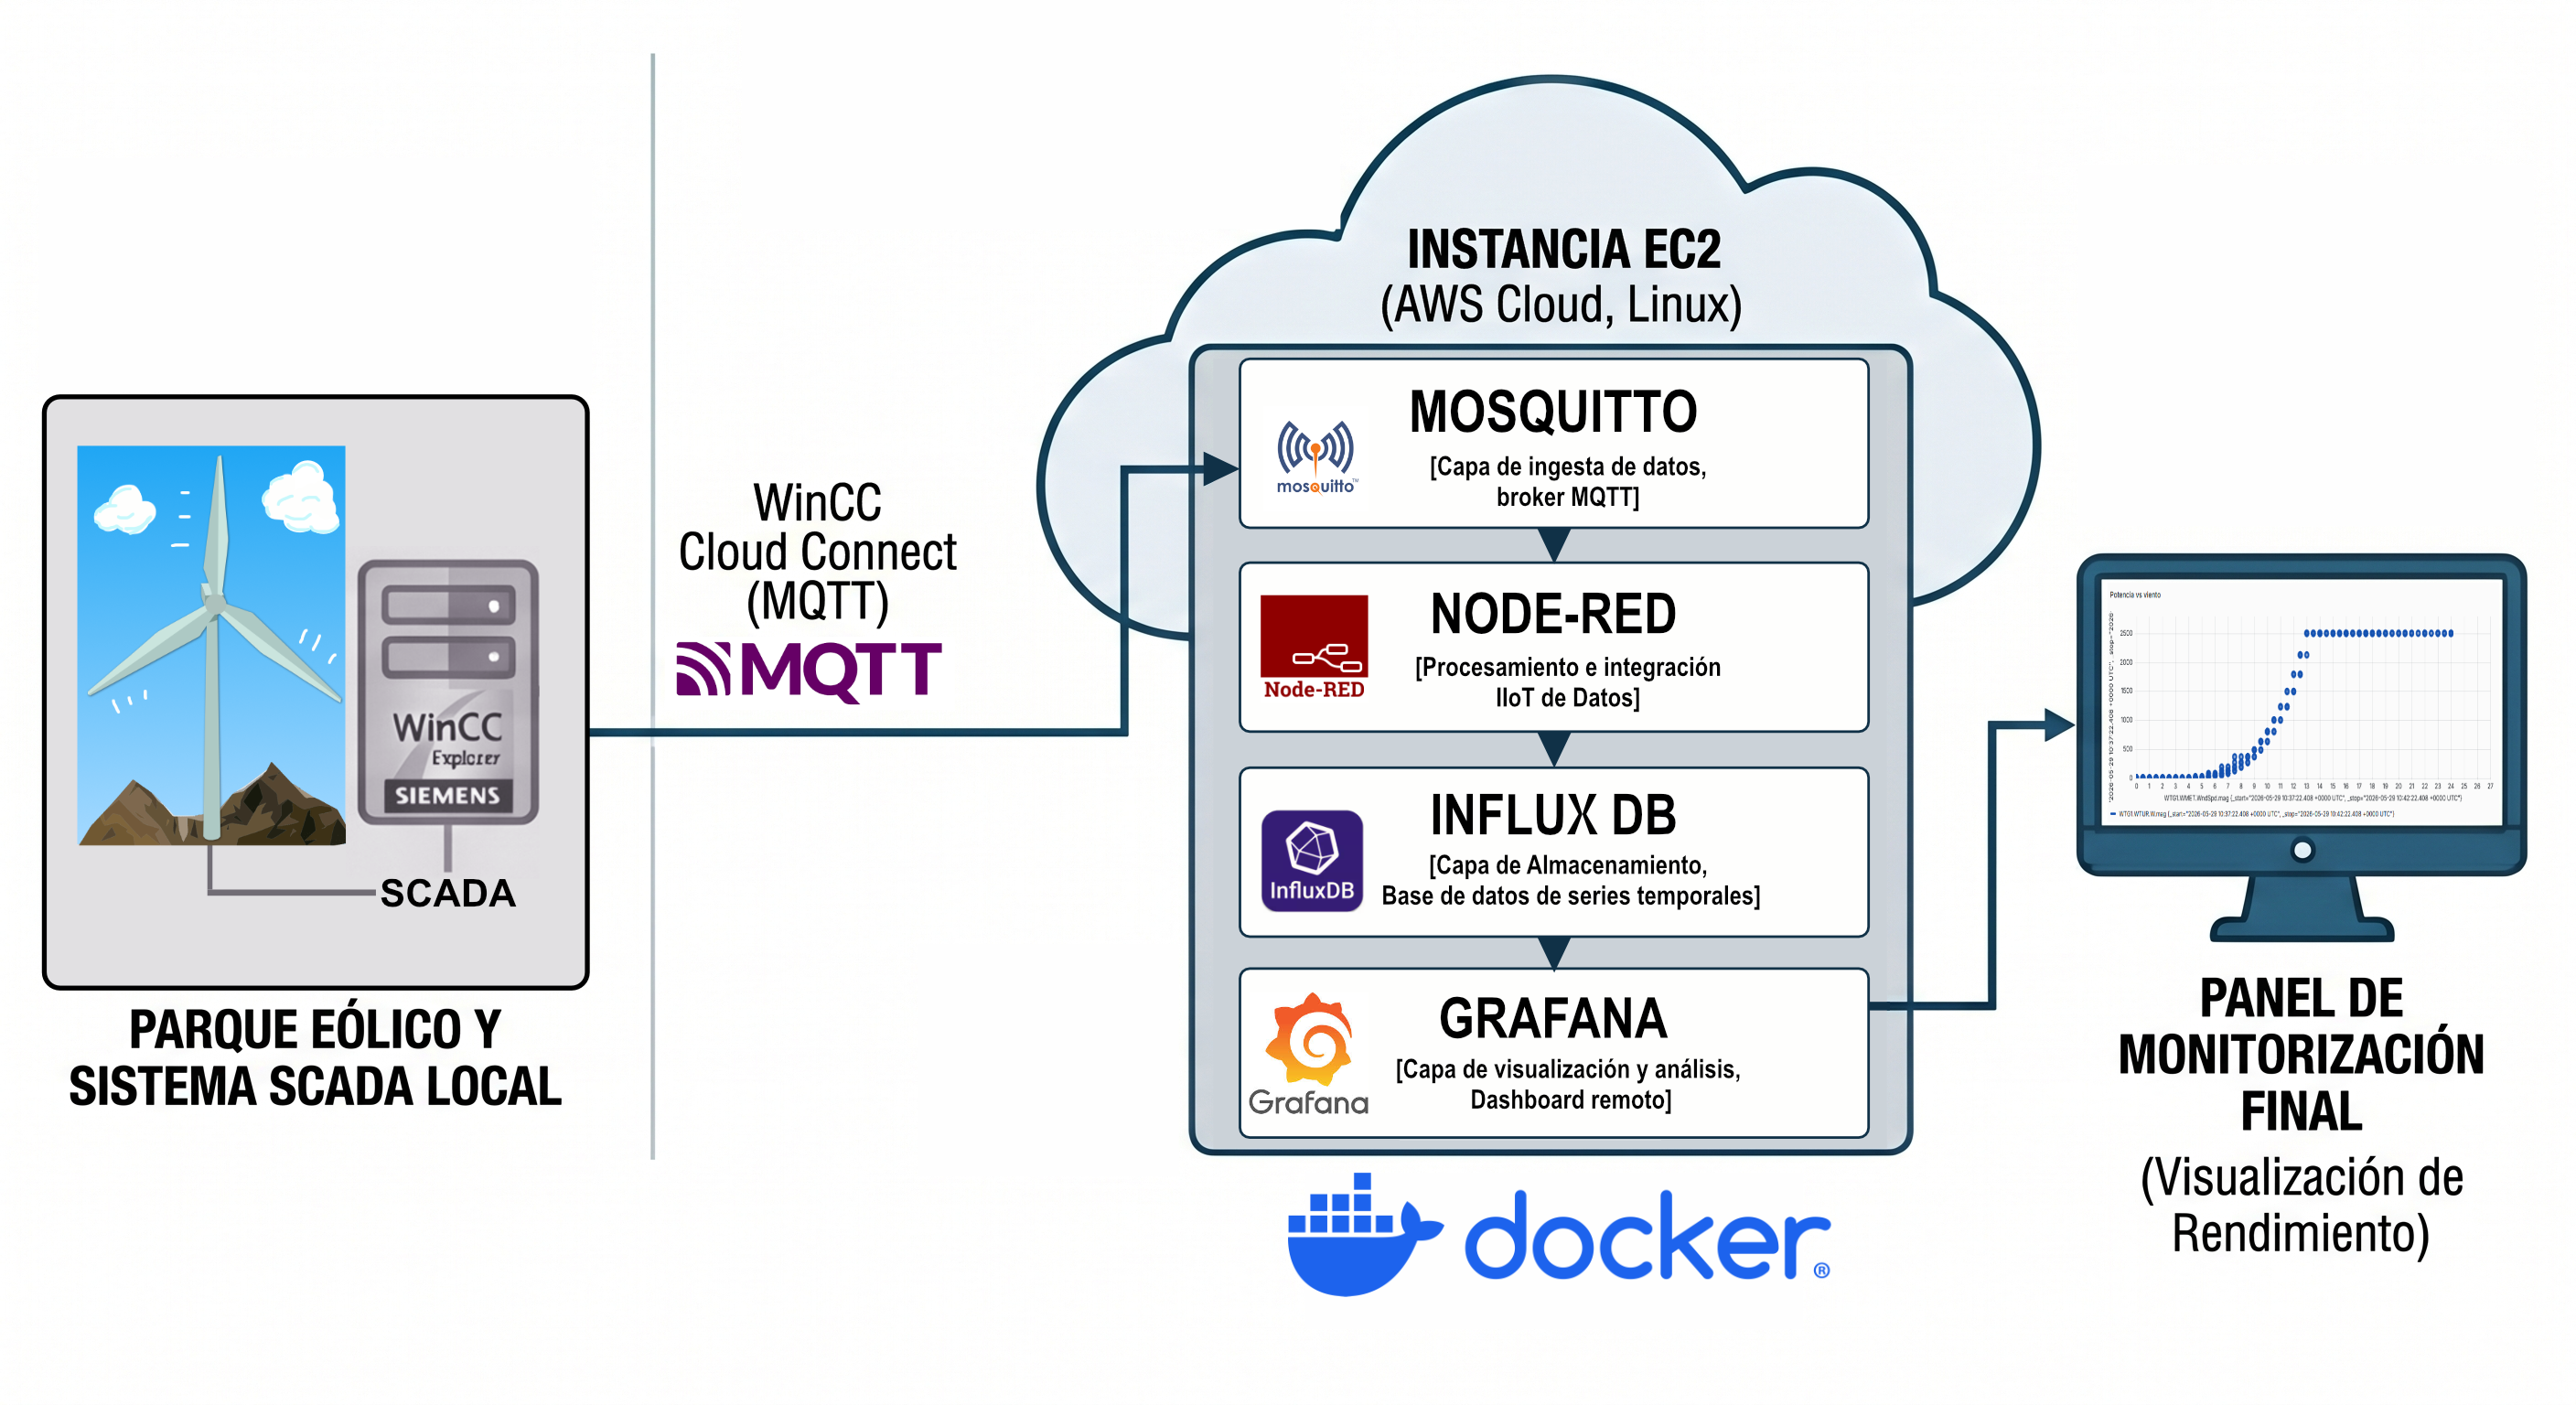
\includegraphics[scale=0.16]{figuras/DiagramaCloud.png}
    \caption{Arquitectura de integración de IIoT para la monitorización de un parque eólico.}
    \label{fig:IIoT}
\end{figure}   

\subsection{Despliegue de la infraestructura en Amazon Web Services (AWS)}

Una vez definida la arquitectura conceptual, el siguiente paso consiste en la materialización de la infraestructura necesaria para soportar el ecosistema IIoT. Para ello, se ha optado por un modelo de Infraestructura como Servicio (IaaS) mediante Amazon Web Services (AWS) ya que a diferencia de otras opciones como Oracle tiene una gran disponibilidad y ofrece un amplio catálogo de servicios gestionados que facilitan el despliegue, la gestión y la escalabilidad de la solución. 
\subsubsection{Instancia EC2}
El núcleo computacional del sistema reside en una instancia de Amazon Elastic Compute Cloud (EC2). Se ha seleccionado una instancia de la familia de microprocesadores t3.medium con un procesador con sistema operativo Ubuntu Server 22.04 LTS, 

\subsubsection{Reglas de entrada del Security Group EC2}
Las reglas de entrada del grupo de seguridad (Security Group) de la instancia EC2 en AWS definen qué tráfico de red está permitido acceder a la instancia. Estas reglas especifican los puertos, protocolos y orígenes que pueden comunicarse con el servidor (tabla \ref{tab:ec2_security_group}).\par
\begin{longtable}[t]{p{2.3cm} p{1cm} p{1.8cm} p{1.2cm} p{1.5cm} p{1.5cm}}
    \caption{Configuración de las reglas de entrada del grupo de seguridad de la instancia EC2.}\\
    \toprule
    \multicolumn{6}{c}{\textbf{Reglas de entrada del Security Group EC2}} \\
    \midrule
    \textbf{ID de regla} & \textbf{IP} & \textbf{Tipo} & \textbf{Proto.} & \textbf{Puertos} & \textbf{Origen}\\
    \midrule
    \endfirsthead

    \toprule
    \multicolumn{6}{c}{\textbf{Reglas de entrada del Security Group EC2 (continuación)}} \\
    \midrule
    \textbf{ID de regla} & \textbf{IP} & \textbf{Tipo} & \textbf{Proto.} & \textbf{Puertos} & \textbf{Origen}\\
    \midrule
    \endhead

    \midrule
    \multicolumn{6}{r}{Continúa en la siguiente página}\\
    \endfoot

    \bottomrule
    
    \label{tab:ec2_security_group}\\
    \endlastfoot

    sgr-014a824e & IPv4 & SSH & TCP & 22 & 0.0.0.0/0\\
    sgr-0b782729 & IPv4 & HTTP & TCP & 80 & 0.0.0.0/0\\
    sgr-0a9de042 & IPv4 & HTTPS & TCP & 443 & 0.0.0.0/0\\
    sgr-0e38166d & IPv4 & TCP Personalizado & TCP & 1880 & 0.0.0.0/0\\
    sgr-0d805336 & IPv4 & TCP Personalizado & TCP & 1883 & 0.0.0.0/0\\
    sgr-09d85840 & IPv4 & TCP Personalizado & TCP & 3000 & 0.0.0.0/0\\
    sgr-03c60e5a & IPv4 & TCP Personalizado & TCP & 8086 & 0.0.0.0/0\\
    sgr-0c3cf32e & IPv4 & TCP Personalizado & TCP & 8883 & 0.0.0.0/0\\
\end{longtable}

\subsubsection{Orquestación de microservicios mediante Docker}
\definecolor{codegreen}{rgb}{0,0.8,0.4}
\definecolor{codegray}{rgb}{0.75,0.75,0.75}
\definecolor{codegold}{rgb}{0.9,0.7,0.15}
\definecolor{codepurple}{rgb}{0.9,0.6,1.0}
\definecolor{backcolour}{rgb}{0.12,0.13,0.20}
\definecolor{textcolor}{rgb}{0.95,0.95,0.95}
\definecolor{codeblue}{rgb}{0,0.4,0.8}
\lstset{
  language=bash,
  rulecolor=\color{backcolour},
    commentstyle=\color{codegreen},
    keywordstyle=\color{codepurple},
    numberstyle=\tiny\color{codegray},
    stringstyle=\color{codegold},
    basicstyle=\ttfamily\footnotesize\color{textcolor},
    breakatwhitespace=false,         
    breaklines=true,                 
    captionpos=b,                    
    keepspaces=false,                
    numbers=left,                    
    numbersep=10pt,                  
    showspaces=false,                
    showstringspaces=false,
    showtabs=false,                  
    tabsize=2,
    frame=none,
    framexleftmargin=0pt,
    framexrightmargin=0pt,
    linewidth=\linewidth,
    columns=fullflexible,
    xleftmargin=0pt,
    lineskip=0pt,
    aboveskip=0.75\baselineskip,
    belowskip=0.75\baselineskip
}
\newenvironment{codeframe}{%
\begin{mdframed}[
    backgroundcolor=backcolour,
    linecolor=backcolour,
    hidealllines=true,
    roundcorner=0pt,
    innerleftmargin=8pt,
    innerrightmargin=8pt,
    innertopmargin=3pt,
    innerbottommargin=0pt,
    skipabove=4pt,
    skipbelow=4pt
]
}{%
\end{mdframed}
}
Para garantizar la portabilidad y escalabilidad de la solución, se ha optado por contenedorizar cada componente de la arquitectura (Node-RED, InfluxDB y Grafana) utilizando Docker, el cual permite empaquetar las aplicaciones junto con sus dependencias en contenedores ligeros que abstraen el sistema operativo sobre el que se ejecutan. De esta forma, las configuraciones especificas de diferentes entornos donde se puedan desplegar los servicios (desarrollo, pruebas, producción) se gestionan de forma consistente y replicable. A continuación se describen los pasos que se han realizado para el despliegue de cada servicio:\par

primero se ha realizado la conexión mediante SSH a la instancia EC2 utilizando un cliente como la terminal de comandos, autenticándose con la clave privada asociada a la instancia. Una vez dentro del entorno de la instancia, se procede a instalar Docker mediante el terminal (listado \ref{cod:instalar_docker})\par\vspace{1cm}
\begin{codeframe}
\begin{lstlisting}[language=bash]
    sudo apt update
    sudo apt install docker.io docker-compose -y
    sudo systemctl start docker
    sudo systemctl enable docker

\end{lstlisting}
\end{codeframe}
\captionof{lstlisting}{Comandos para la instalación de Docker en la instancia EC2.}
\label{cod:instalar_docker}
\vspace{1cm}
El despliegue se ha automatizado mediante un archivo de configuración Docker-compose.yml, que actúa como orquestador de la solución. Este archivo define no solo las imágenes de software a utilizar, sino también dos elementos fundamentales para la integridad industrial(listado \ref{cod:docker-compose}):
\begin{itemize}
    \item Red Interna Virtual (Docker Network): Se ha creado una red privada aislada (scada\_net) para que los contenedores se comuniquen entre sí (por ejemplo, Node-RED enviando datos a InfluxDB) sin exponer dichos puertos al internet público, reduciendo significativamente la superficie de ataque.
    \item Persistencia de Datos (Docker Volumes): Dado que los contenedores son efímeros por naturaleza, se han configurado volúmenes vinculados al almacenamiento físico de la instancia EC2. Esto garantiza que, ante un reinicio del sistema o una actualización del software, los datos históricos del parque eólico y las configuraciones de los dashboards no se pierdan.
\end{itemize}

\begin{codeframe}
\begin{lstlisting}[language=bash]
    version: '3.8'

services:
    # Base de Datos de Series Temporales
  influxdb:
    image: influxdb:2.7
    container_name: influxdb_scada
    restart: always
    ports:
      - "8086:8086"
    volumes:
      - influxdb_data:/var/lib/influxdb2
    networks:
      - scada_net

    # Motor de flujos y procesamiento de datos
  nodered:
    image: nodered/node-red:latest
    container_name: nodered_scada
    restart: always
    ports:
      - "1880:1880"
    volumes:
      - nodered_data:/data
    depends_on:
      - influxdb
    networks:
      - scada_net

    # Visualizacion de datos
  grafana:
    image: grafana/grafana:latest
    container_name: grafana_scada
    restart: always
    ports:
      - "3000:3000"
    volumes:
      - grafana_data:/var/lib/grafana
    depends_on:
      - influxdb
    networks:
      - scada_net

networks:
  scada_net:
    driver: bridge

volumes:
  influxdb_data:
  nodered_data:
  grafana_data:
\end{lstlisting}
\end{codeframe}
\captionof{lstlisting}{Archivo Docker Compose para el despliegue de la arquitectura IIoT en AWS.}
\label{cod:docker-compose}
\vspace{1cm}
Se ha levantado el entorno de contenedores mediante la terminal (listado \ref{cod:levantar_contenedores}):\vspace{1cm}\par
\begin{codeframe}
\begin{lstlisting}[language=bash]
    sudo docker-compose up -d
\end{lstlisting}
\end{codeframe}
\captionof{lstlisting}{Comando para iniciar los servicios definidos en el archivo Docker Compose.}
\label{cod:levantar_contenedores}
\vspace{1cm}
Una vez se han levantado los contenedores, se ha configurado el acceso del servicio Cloud Connect de WinCC (figura \ref{fig:cloud_connect}) para publicar los datos en el broker MQTT (puerto 1883) de la instancia EC2 utilizando la direccion IP publica de la instancia EC2 (\texttt{13.60.146.240}) (figura \ref{fig:aws}).\\ \par
\begin{figure}[t]
    \centering
    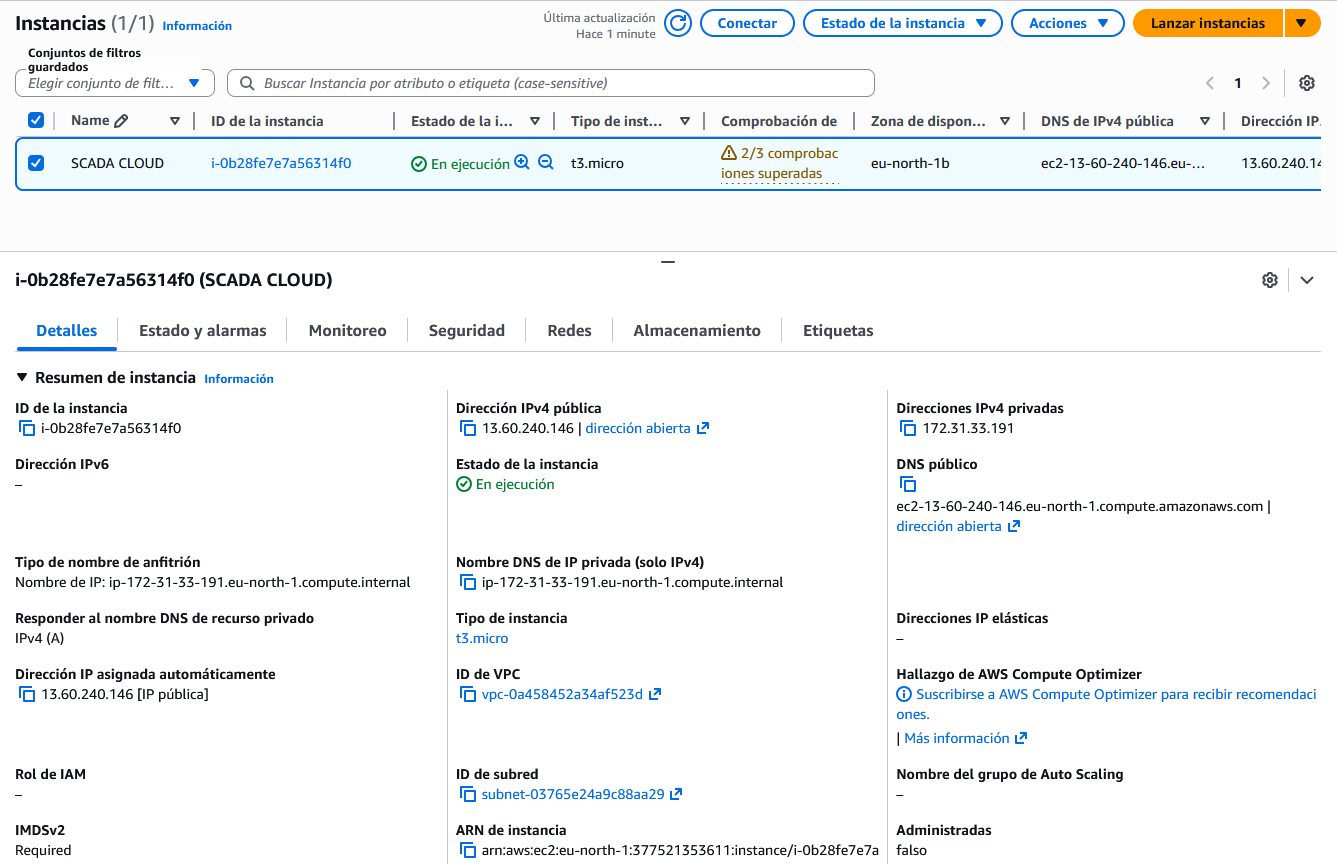
\includegraphics[scale=0.4]{figuras/aws.png}
    \caption{Arquitectura de integración de IIoT para la monitorización de un parque eólico.}
    \label{fig:aws}
\end{figure}
\begin{figure}[t]
    \centering
    \includegraphics[scale=0.6]{figuras/cloudconnect.png}
    \caption{Configuración del módulo Cloud Connect de WinCC para la publicación de datos en el broker MQTT de la instancia EC2.}
    \label{fig:cloud_connect}
\end{figure}
\vspace{1cm}
Ahora en cualquier navegador web se puede acceder al servicio de Node-RED utilizando la uri \hspace{0.5cm}\url{http://13.60.146.240:1880}. En este servicio se han configurado las suscripciones a los tópicos MQTT. Se ha realizado mediante un nodo MQTT de tipo "Subscribe" con la dirección del broker MQTT de la instancia EC2, junto con el tópico configurado en Cloud Connect. Posteriormente, se añaden nodos de función para transformar los datos recibidos y un nodo de salida para insertar los datos en InfluxDB (\ref{fig:nodered}).\\ \par

\begin{figure}[t]
    \centering
    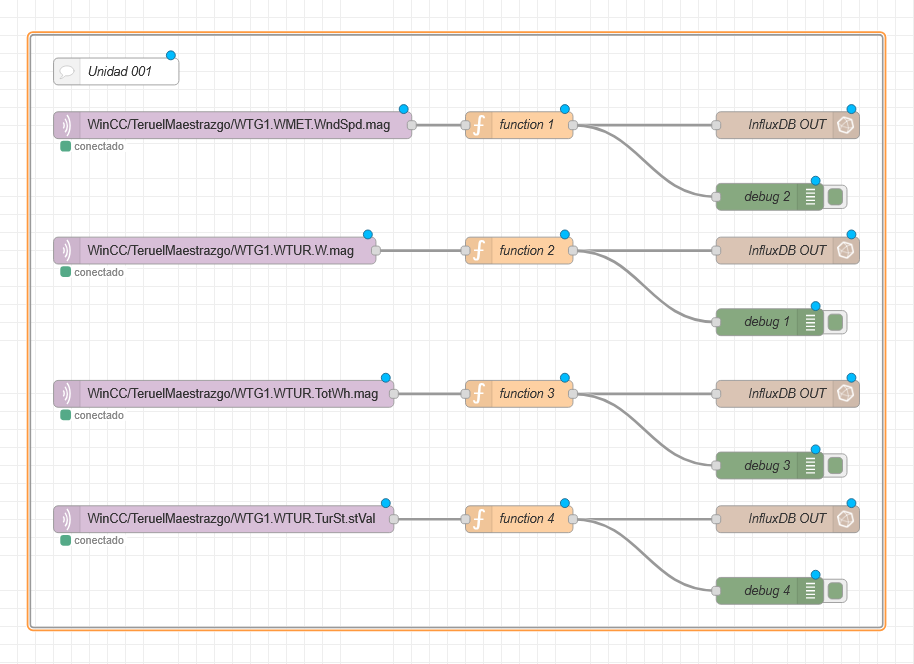
\includegraphics[scale=0.5]{figuras/NodeRedMQTT.png}
    \caption{Configuración de Node-RED para la suscripción a tópicos MQTT y procesamiento de datos antes de su inserción en InfluxDB.}
    \label{fig:nodered}
\end{figure}

Se puede acceder al servicio de InfluxDB a través del uri\hspace{0.5cm} \url{http://13.60.240.146:8086}. para configurar la base de datos y los buckets necesarios para almacenar los datos del parque eólico.\\\par 

Finalmente, se accede a Grafana mediante la uri\hspace{0.5cm}\url{http://13.60.240.146:3000} para configurar el panel de visualización de los datos almacenados en InfluxDB. Para ello, se selecciona la fuente de datos InfluxDB utilizando la dirección \url{http://13.60.240.146:8086}.y el token de autenticación.(ver figura \ref{fig:grafana_config})\\\par
\begin{figure}[t]
    \centering
    \includegraphics[scale=1]{figuras/grafana_config.png}
    \caption{Configuración de Grafana para la conexión a InfluxDB como fuente de datos.}
    \label{fig:grafana_config}
\end{figure}
\vspace{1cm}
Una vez configurada la fuente de datos, se crean los dashboards personalizados para la monitorización del parque eólico, utilizando las consultas a InfluxDB para mostrar variables como la velocidad del viento, potencia generada, estados de los aerogeneradores, entre otros indicadores clave de rendimiento (KPIs) relevantes para la operación y mantenimiento del parque eólico.\\\par

\section{Ciberseguridad IEC 62443-4-2:2019}
Esta sección es una directriz de seguridad válida para SIMATIC HMI WinCC V8.1 que describe sus funciones de ciberseguridad. Sigue la norma IEC 62443-4-2:2019 de ciberseguridad para sistemas de automatización y control industrial. La norma IEC 62443 define cuatro niveles de seguridad (SL, por sus siglas en inglés) distintos, basados en los recursos, las habilidades y la motivación del posible atacante:

\begin{itemize}
    \item \textbf{SL 1:} Protección contra vulneraciones casuales/accidentales:
    Protección contra el acceso no autorizado por parte de alguien sin intención maliciosa.
    \item \textbf{SL 2:} Protección contra vulneraciones intencionadas con medios sencillos:
    Protección contra ataques genéricos y de bajos recursos.
    \item \textbf{SL 3:} Protección contra ataques sofisticados:
    Protección contra atacantes (hackers) con recursos moderados, motivación moderada y conocimientos específicos sobre Sistemas de Automatización y Control Industrial (IACS, por sus siglas en inglés).
    \item \textbf{SL 4:} Protección contra ataques altamente sofisticados / de Estados-nación:
    Protección contra atacantes con amplios recursos, alta motivación y profunda experiencia en IACS.
\end{itemize}

Los requisitos fundacionales (FR) son los requisitos de seguridad que deben cumplirse para alcanzar  el SL específico. Estos requisitos se dividen en siete categorías principales, cada una con sub-requisitos específicos. A continuación se describen los requisitos fundacionales para cada nivel de seguridad:\par
\subsection{FR1: Identificación y autenticación de usuarios (IAC)}
\begin{enumerate}
    \item[] \textbf{Identificación y autenticación de usuarios (CR1.1)}
    
    \begin{itemize}
        \item CR1.1: Acceso limitado a aplicaciones de WinCC V8.1 mediante grupos de usuarios de Windows. Acceso restringido de datos del runtime mediante grupos de usuarios de WinCC. (SL 1)
        \item RE 1:Identificación única de usuarios mediante ID única, creación de roles con permisos específicos. (SL 2)
        \item RE 2(No ofertado): Autenticación multifactorial para todas las interfaces (SL 3-4).
    \end{itemize}
    
    Nivel de seguridad SL-T 2 : Requerimientos CR1.1 + RE 1 .\par

    \item[] \textbf{Identificación y autenticación de dispositivos (CR1.2)}
    
    \begin{itemize}
        \item CR1.2:    Identificación y autenticación de dispositivos básica(SL 2)
        \item RE 1: Identificación única de dispositivos mediante certificados digitales o credenciales seguras, Integrado en comunicaciónes OPC UA. (SL 3-4)
       
    \end{itemize}

    Nivel de seguridad SL-T 4: Requerimientos CR1.2 + RE 1.\par

    \item[] \textbf{Gestión de cuentas (CR1.3)}
    
    \begin{itemize}
        \item CR1.3:  Gestión de cuentas mediante:  1-User Administrator, 2-WinCC UserAdminControl, 3-SIMATIC Logon. (SL 1-4).
       
    \end{itemize}

    Nivel de seguridad SL-T 4: Requerimientos CR1.3.\par


    \item[] \textbf{Gestión de IDs (CR1.4)}
    
    \begin{itemize}
        \item CR1.4: Politica de identificación unica y sistematica  (SL 1-4).
       
    \end{itemize}
    Nivel de seguridad SL-T 4: Requerimientos CR1.4.\par

     \item[] \textbf{Gestión de autenticación (CR1.5)}
    
    \begin{itemize}
        \item CR1.5: Registros de eventos de autenticación, Contraseñas encriptadas,   (SL 1-2).
       \item RE 1(No ofertado): Seguridad de hardware para autenticación (SL 3-4).
    \end{itemize}
    Nivel de seguridad SL-T 2: Requerimientos CR1.5.\par

    \item[] \textbf{Fuerza de autenticación basada en contraseñas (CR1.7)}
    
    \begin{itemize}
        \item CR1.7: Contraseñas con complejidad mínima (SL 1-2).
       \item RE 1(No ofertado): Caducidad de contraseñas para humanos(SL 3).
       \item RE 2(No ofertado): Caducidad de contraseñas para dispositivos, humanos y software (SL 4).
    \end{itemize}
    Nivel de seguridad SL-T 2: Requerimientos CR1.7.\par

    \item[]  \textbf{Infraestructura de clave pública (CR1.8)}
    
    \begin{itemize}
        \item CR1.8:Protocolos de comunicación con uso de certificados digitales (SL 2-4).
    \end{itemize}
    Nivel de seguridad SL-T 4: Requerimientos CR1.8.\par
    
  \item[] \textbf{Retroalimentación de autenticación (CR1.10)}
    
    \begin{itemize}
        \item CR1.10: No revelación de información sensible para asistencia de autenticación a un intruso. Contraseña oculta por caracteres "****", tamaño no revelado.(SL 1-4).
    \end{itemize}
    Nivel de seguridad SL-T 4: Requerimientos CR1.10.\par
 \item[] \textbf{Autenticación fallida (CR1.11)}
    
    \begin{itemize}
        \item CR1.11: Limitación del número de intentos de autenticación fallida antes de bloqueo.(SL 1-4).
    \end{itemize}
    Nivel de seguridad SL-T 4: Requerimientos CR1.11.\par

\item[] \textbf{Autenticación fallida (CR1.11)}
    
    \begin{itemize}
        \item CR1.11: Limitación del número de intentos de autenticación fallida antes de bloqueo.(SL 1-4).
    \end{itemize}
    Nivel de seguridad SL-T 4: Requerimientos CR1.11.\par


\item[] \textbf{Notificaciones de uso de sistema (CR1.12)}
    
    \begin{itemize}
        \item CR1.12: Notificaciones limitadas a grupos de usuarios.(SL 1-4).
    \end{itemize}
    Nivel de seguridad SL-T 4: Requerimientos CR1.12.\par

\item[] \textbf{Fuerza de contraseña secreta compartida (CR1.13)}
    
    \begin{itemize}
        \item CR1.13: Implementación de políticas de complejidad para contraseñas compartidas.(SL 2).
        \item RE 1(No ofertado): Contraseñas encriptadas por hardware.(SL 3-4).
    \end{itemize}
    Nivel de seguridad SL-T 2: Requerimientos CR1.13.\par
\end{enumerate}


\subsection{FR 2: Control de uso}
\begin{enumerate}
    \item[] \textbf{Refuerzo de control de acceso (CR2.1)}
    
    \begin{itemize}
        \item CR2.1: Acceso restringido a usuarios humanos sobre recursos y funciones. (SL 1).
        \item RE 1: Control de acceso a todos los usuarios procesos y dispositivos mediante identificación.(SL 2).
        \item RE 2 Control de acceso basado en roles .(SL 2).
        \item RE 3: Acusado de emergencia  mediante requerimiento de supervisor(SL 3).
        \item RE 4(No ofertado): Acusación de alarmas siempre por dos usuarios distinto (SL 4).
    \end{itemize}
    Nivel de seguridad SL-T 3: Requerimientos CR2.1. + RE1 +RE2 +RE3.\par
    
    \item[] \textbf{Refuerzo de control de acceso inalambrico (CR2.2)}
    No procede.
    \par

    \item[] \textbf{Presistencia de sesión (CR2.5)}
    
    \begin{itemize}
        \item CR2.5: Log out tras periodo de inactividad (SL 1-4).
       
    \end{itemize}
    Nivel de seguridad SL-T 4: Requerimientos CR2.5.\par

     \item[] \textbf{Terminación de sesión para clientes (CR2.6)}
    
    \begin{itemize}
        \item CR2.6: Cierre de sesión automático tras periodo de inactividad (SL 2-4).
       
    \end{itemize}
    Nivel de seguridad SL-T 4: Requerimientos CR2.6.\par
 \item[] \textbf{Limitación de sesiones activas (CR2.7)}
    
    \begin{itemize}
        \item CR2.7: Limitacion de acceso a clientes WEB(SL 3-4).
       
    \end{itemize}
    Nivel de seguridad SL-T 4: Requerimientos CR2.7.\par
    \item[] \textbf{Eventos auditables (CR2.8)}
    
    \begin{itemize}
        \item CR2.8: Registro de eventos auditables (SL 1-4).
       
    \end{itemize}
    Nivel de seguridad SL-T 4: Requerimientos CR2.8.\par
\item[] \textbf{Capacidad de almacenamiento de auditoría (CR2.9)}
    
    \begin{itemize}
        \item CR2.9: Existencia de capacidad de almacenamiento de auditoría (SL 1-2).
       \item RE 1: Notificación de umbral de almacenamiento de auditoría (SL 3-4).
    \end{itemize}
    Nivel de seguridad SL-T 4: Requerimientos CR2.9.\par

\item[] \textbf{Capacidad de almacenamiento de auditoría (CR2.9)}
    
    \begin{itemize}
        \item CR2.9: Existencia de capacidad de almacenamiento de auditoría (SL 1-2).
       \item RE 1: Notificación de umbral de almacenamiento de auditoría (SL 3-4).
    \end{itemize}
    Nivel de seguridad SL-T 4: Requerimientos CR2.9.\par
\end{enumerate}

\subsection{Matriz de implementación de requisitos y niveles de seguridad}

A continuación se presenta una tabla basada en FR1 (IAC) de la IEC 62443-4-2:2019:
\begin{longtable}{p{4.1cm} c c c c c}
    \toprule
    \textbf{Requisito ID} & \multicolumn{4}{c}{\textbf{Nivel de seguridad}} & \textbf{SL-T} \\
    \midrule
    \endfirsthead

    \toprule
    \textbf{Requisito ID} & \multicolumn{4}{c}{\textbf{Nivel de seguridad}} & \textbf{SL-A} \\
    \cmidrule(lr){2-5}
    \midrule
    \endhead

    \midrule
    \multicolumn{6}{r}{Continúa en la siguiente página}\\
    \endfoot

    \bottomrule
    \endlastfoot

    \multicolumn{6}{c}{\textbf{FR 1: Identificación y autenticación de usuarios (IAC)}} \\
    \midrule
    CR 1.1 & 1 & 2 & 3 & 4 & $\checkmark$ \\
    CR 1.1 RE (1) & --- & 2 & 3 & 4 & $\checkmark$ \\
    CR 1.1 RE (2) & --- & --- & 3 & 4 & $\times$ \\
    \cmidrule(lr){1-6}
    \multicolumn{6}{l}{\textit{nivel SL-T maximo alcanzable (CR 1.1): 2}} \\
    \midrule
    CR 1.2 & --- & 2 & 3 & 4 & $\checkmark$ \\
    CR 1.2 RE (1) & --- & --- & 3 & 4 & $\checkmark$ \\
    \cmidrule(lr){1-6}
    \multicolumn{6}{l}{\textit{nivel SL-T maximo alcanzable (CR 1.2): 4}} \\
    \midrule
    CR 1.3 & 1 & 2 & 3 & 4 & $\checkmark$ \\
    \cmidrule(lr){1-6}
    \multicolumn{6}{l}{\textit{nivel SL-T maximo alcanzable (CR 1.3): 4}} \\
    \midrule
    CR 1.4 & 1 & 2 & 3 & 4 & $\checkmark$ \\
    \cmidrule(lr){1-6}
    \multicolumn{6}{l}{\textit{nivel SL-T maximo alcanzable (CR 1.4): 4}} \\
    \midrule
    CR 1.5 & 1 & 2 & 3 & 4 & $\checkmark$ \\
    CR 1.5 RE (1) & --- & --- & 3 & 4 & $\times$ \\
    \cmidrule(lr){1-6}
    \multicolumn{6}{l}{\textit{nivel SL-T maximo alcanzable (CR 1.5): 2}} \\
    \midrule
    NDR 1.6 & 1 & 2 & 3 & 4 & $\times$ \\
    NDR 1.6 RE (1) & --- & 2 & 3 & 4 & $\times$ \\
    \cmidrule(lr){1-6}
    \multicolumn{6}{l}{\textit{nivel SL-T maximo alcanzable (NDR 1.6): N/A}} \\
    \midrule
    CR 1.7 & 1 & 2 & 3 & 4 & $\checkmark$ \\
    CR 1.7 RE (1) & --- & --- & 3 & 4 & $\times$ \\
    CR 1.7 RE (2) & --- & --- & --- & 4 & $\times$ \\
    \cmidrule(lr){1-6}
    \multicolumn{6}{l}{\textit{nivel SL-T maximo alcanzable (CR 1.7): 2}} \\
    \midrule
    CR 1.8 & --- & 2 & 3 & 4 & $\checkmark$ \\
    \cmidrule(lr){1-6}
    \multicolumn{6}{l}{\textit{nivel SL-T maximo alcanzable (CR 1.8): 4}} \\
    \midrule
    CR 1.9 & --- & 2 & 3 & 4 & $\checkmark$ \\
    CR 1.9 RE (1) & --- & --- & 3 & 4 & $\times$ \\
    \cmidrule(lr){1-6}
    \multicolumn{6}{l}{\textit{nivel SL-T maximo alcanzable (CR 1.9): 2}} \\
    \midrule
    CR 1.10 & 1 & 2 & 3 & 4 & $\checkmark$ \\
    \cmidrule(lr){1-6}
    \multicolumn{6}{l}{\textit{nivel SL-T maximo alcanzable (CR 1.10): 4}} \\
    \midrule
    CR 1.11 & 1 & 2 & 3 & 4 & $\checkmark$ \\
    \cmidrule(lr){1-6}
    \multicolumn{6}{l}{\textit{nivel SL-T maximo alcanzable (CR 1.11): 4}} \\
    \midrule
    CR 1.12 & 1 & 2 & 3 & 4 & $\checkmark$ \\
    \cmidrule(lr){1-6}
    \multicolumn{6}{l}{\textit{nivel SL-T maximo alcanzable (CR 1.12): 4}} \\
    \midrule
    NDR 1.13 & 1 & 2 & 3 & 4 & $\times$ \\
    NDR 1.13 RE (1) & --- & --- & 3 & 4 & $\times$ \\
    \cmidrule(lr){1-6}
    \multicolumn{6}{l}{\textit{nivel SL-T maximo alcanzable (NDR 1.13): N/A}} \\
    \midrule
    CR 1.14 & --- & --- & --- & 4 & $\times$ \\
    \cmidrule(lr){1-6}
    \multicolumn{6}{l}{\textit{nivel SL-T maximo alcanzable (CR 1.14): N/A}} \\
    \midrule
    \multicolumn{6}{c}{\textbf{FR 2: Control de uso (UC)}} \\
    \midrule
    CR 2.1 & 1 & 2 & 3 & 4 & $\checkmark$ \\
    CR 2.1 RE (1) & --- & 2 & 3 & 4 & $\checkmark$ \\
    CR 2.1 RE (2) & --- & 2 & 3 & 4 & $\checkmark$ \\
    CR 2.1 RE (3) & --- & --- & 3 & --- & $\checkmark$ \\
    CR 2.1 RE (4) & --- & --- & --- & 4 & $\times$ \\
    \cmidrule(lr){1-6}
    \multicolumn{6}{l}{\textit{nivel SL-T maximo alcanzable (CR 2.1): 3}} \\
    \midrule
    CR 2.2 & 1 & 2 & 3 & 4 & $\times$ \\
    \cmidrule(lr){1-6}
    \multicolumn{6}{l}{\textit{nivel SL-T maximo alcanzable (CR 2.2): N/A}} \\
    \midrule
    CR 2.3 & --- & --- & --- & --- & $\times$ \\
    \cmidrule(lr){1-6}
    \multicolumn{6}{l}{\textit{nivel SL-T maximo alcanzable (CR 2.3): N/A}} \\
    \midrule
    SAR 2.4 & 1 & 2 & 3 & 4 & $\times$ \\
    SAR 2.4 RE (1) & --- & 2 & 3 & 4 & $\times$ \\
    \cmidrule(lr){1-6}
    \multicolumn{6}{l}{\textit{nivel SL-T maximo alcanzable (SAR 2.4): N/A}} \\
    \midrule
    EDR 2.4 & 1 & 2 & 3 & 4 & $\times$ \\
    EDR 2.4 RE (1) & --- & 2 & 3 & 4 & $\times$ \\
    \cmidrule(lr){1-6}
    \multicolumn{6}{l}{\textit{nivel SL-T maximo alcanzable (EDR 2.4): N/A}} \\
    \midrule
    HDR 2.4 & 1 & 2 & 3 & 4 & $\times$ \\
    HDR 2.4 RE (1) & --- & 2 & 3 & 4 & $\times$ \\
    \cmidrule(lr){1-6}
    \multicolumn{6}{l}{\textit{nivel SL-T maximo alcanzable (HDR 2.4): N/A}} \\
    \midrule
    NDR 2.4 & 1 & 2 & 3 & 4 & $\times$ \\
    NDR 2.4 RE (1) & --- & 2 & 3 & 4 & $\times$ \\
    \cmidrule(lr){1-6}
    \multicolumn{6}{l}{\textit{nivel SL-T maximo alcanzable (NDR 2.4): N/A}} \\
    \midrule
    CR 2.5 & 1 & 2 & 3 & 4 & $\checkmark$ \\
    \cmidrule(lr){1-6}
    \multicolumn{6}{l}{\textit{nivel SL-T maximo alcanzable (CR 2.5): 4}} \\
    \midrule
    CR 2.6 & --- & 2 & 3 & 4 & $\checkmark$ \\
    \cmidrule(lr){1-6}
    \multicolumn{6}{l}{\textit{nivel SL-T maximo alcanzable (CR 2.6): 4}} \\
    \midrule
    CR 2.7 & --- & --- & 3 & 4 & $\checkmark$ \\
    \cmidrule(lr){1-6}
    \multicolumn{6}{l}{\textit{nivel SL-T maximo alcanzable (CR 2.7): 4}} \\
    \midrule
    CR 2.8 & 1 & 2 & 3 & 4 & $\checkmark$ \\
    \cmidrule(lr){1-6}
    \multicolumn{6}{l}{\textit{nivel SL-T maximo alcanzable (CR 2.8): 4}} \\
    \midrule
    CR 2.9 & 1 & 2 & 3 & 4 & $\checkmark$ \\
    CR 2.9 RE (1) & --- & --- & 3 & 4 & $\checkmark$ \\
    \cmidrule(lr){1-6}
    \multicolumn{6}{l}{\textit{nivel SL-T maximo alcanzable (CR 2.9): 4}} \\
    \midrule
    CR 2.10 & 1 & 2 & 3 & 4 & $\checkmark$ \\
    \cmidrule(lr){1-6}
    \multicolumn{6}{l}{\textit{nivel SL-T maximo alcanzable (CR 2.10): 4}} \\
    \midrule
    CR 2.11 & 1 & 2 & 3 & 4 & $\checkmark$ \\
    CR 2.11 RE (1) & --- & 2 & 3 & 4 & $\checkmark$ \\
    CR 2.11 RE (2) & --- & --- & --- & 4 & $\checkmark$ \\
    \cmidrule(lr){1-6}
    \multicolumn{6}{l}{\textit{nivel SL-T maximo alcanzable (CR 2.11): 4}} \\

    \caption{Tabla FR1 y FR2 basada en IEC 62443-4-2:2019. Las columnas de nivel muestran el número de nivel aplicable y la columna SL-A indica si el requerimiento se cumple en la solución ($\checkmark$) o no ($\times$).}
    \label{tab:fr1_iac_slt}\\
\end{longtable}


\textbf{Conclusión:} La implementación actual de WinCC V8.1 en la solución propuesta alcanza un nivel de seguridad SL 2, con capacidades parciales para SL 3 mediante la adecuada configuración de la segmentación de red y los mecanismos de detección.

\chapter{Análisis de resultados (si procede)}
\label{cap:analisis_de_resultados}

En este capítulo se presentan resultados de la solución implementada, incluyendo métricas de rendimiento, análisis de latencia extremo a extremo  todo ello probado con el modelo de simulación del aerogenerador especificado en el anexo \ref{cap:Pruebas}.

\section{Pruebas unitarias y de integración}

\section{Análisis de Rendimiento de los Procesos del SCADA}
\label{subsec:rendimiento_scada}
Para verificar la eficiencia y la carga computacional del \ac{SCADA}, se  ha realizado un análisis del proceso \texttt{PDLrt.exe}. \texttt{PDLrt.exe} es el motor encargado de la interfaz gráfica de usuario (HMI). Procesa el renderizado de las pantallas, la actualización de las animaciones dinámicas de las turbinas y la navegación del operador en tiempo real. La monitorización se llevó a cabo mediante la herramienta \textit{Windows Performance Monitor (PerfMon)}, evaluando el impacto en la \ac{CPU} y el comportamiento de la \ac{RAM} componente durante el régimen operativo nominal del parque eólico.\\\par

Para ello se han analizado dos escenarios de carga computacional, el primero una carga de idle y el segundo una carga de estres. La carga de idle se ha definido como el estado del sistema en las pantallas que no presentan animaciones dinámicas ni actualizaciones frecuentes de variables (\texttt{11\_SUB\_General}). Mientras que la carga de estrés se ha configurado con la pantalla de supervisión principal (\texttt{10\_WTG\_Overview}), que incluye animaciones en tiempo real de las turbinas y actualizaciones constantes de los indicadores clave de rendimiento (KPIs) del parque con el máximo posible de aerogeneradores (57) en la visualización.\\\par

El análisis se ha realizado en un entorno virtualizado con las características de hardware indicadas en la tabla \ref{tab:hardware_mv}.\par


\begin{table}[!tbp]
\centering
\caption{Especificaciones del entorno de hardware y virtualización.}
\label{tab:hardware_mv}
\resizebox{\textwidth}{!}{
\begin{tabular}{ll}
\hline
\textbf{Componente / Parámetro} & \textbf{Descripción Técnica} \\ \hline
\textbf{Equipo Anfitrión (Host)} & ASUS TUF Gaming A15 \\
\textbf{Procesador Físico (CPU Host)} & AMD Ryzen 7 7435HS $3.1$ GHz \\
\textbf{Arquitectura de Virtualización} & VM Ware \\
\textbf{Núcleos Asignados a la MV} & $4$ Núcleos virtuales (vCPUs) de 8 disponibles\\
\textbf{Memoria RAM Asignada} & $8.0$ GB DDR5 \\
\textbf{Sistema Operativo Invitado} & Windows 10 Pro \\ \hline
\end{tabular}
}
\end{table}

El perfil de consumo y la distribución de carga de hardware de forma individualizada se consolidan en la Tabla~\ref{tab:procesos_scada}.

\begin{table}[!tbp]
\centering
\caption{Métricas de rendimiento e impacto computacional de los procesos del SCADA.}
\label{tab:procesos_scada}
\resizebox{\textwidth}{!}{% Adaptación automática al ancho de página si es necesario
\begin{tabular}{llccc}
\hline
\textbf{Proceso} & \textbf{Cantidad de Tags} & \textbf{ \% CPU (Idle)} & \textbf{\%CPU (CEstrés)} & \textbf{  RAM (KB)} \\ \hline
\texttt{PdlRT.exe } &  10983 & $2.87\%$ & $16.21\%$& $141.054$  \\
\texttt{PdlRT.exe } &  23703 & $3.02\%$ & $18.20\%$& $3.02\%$ \\
\texttt{PdlRT.exe } &  40875 & $3.09\%$ & $19.76\%$ & $3.09\%$ \\
\bottomrule
\end{tabular}
}
\end{table}

Debido a que el proceso \texttt{PdlRT.exe} es un proceso Monohilo se ha diseñado un experimento de estres para evaluar su comportamiento bajo una carga creciente centrandose en un único nucleo del procesador (\ref{fig:Stress}).\par

\begin{figure}[!tpb]
    \centering
    \includegraphics[width=\textwidth]{figuras/carga.png}
    \caption{Evolución del consumo de CPU del proceso \texttt{PdlRT.exe} bajo una carga creciente de tags.}
    \label{fig:Stress}
\end{figure}

\section{Evaluación de la Latencia Extremo a Extremo (End-to-End)}
Para validar la aptitud de la arquitectura IIoT en tareas de supervisión y analítica predictiva en tiempo real mitigado (\textit{near real-time}), se diseñó un ensayo empírico de caracterización del retraso temporal en el flujo de datos. El experimento consistió en la inyección de $N = 1000$ eventos de cambio de estado aleatorios en las variables de simulación de campo, registrando la marca de tiempo de origen ($t_{origen}$) bajo el estándar \textit{OPC UA}.\par 

La latencia total de la arquitectura ($T_{E2E}$) se define formalmente según la Ecuación~\ref{eq:latencia}:

\begin{equation}
    T_{E2E} = t_{campo} + t_{edge} + t_{red} + t_{cloud}
    \label{eq:latencia}
\end{equation}

Tras recuperar los registros persistidos en la instancia de \textit{InfluxDB} en \textit{AWS}, se contrastó el tiempo de almacenamiento definitivo ($t_{registro}$) frente al de origen. Los resultados estadísticos del retraso acumulado se presentan en la Tabla~\ref{tab:resultados_latencia}.

\begin{table}[htbp]
\centering
\caption{Desglose estadístico de los tiempos de latencia y retardo por etapas de la arquitectura (Valores en milisegundos).}
\label{tab:resultados_latencia}
\resizebox{\textwidth}{!}{
\begin{tabular}{lcccc}
\toprule
\textbf{Etapa del Flujo (Componente)} & \textbf{Mínimo (ms)} & \textbf{Máximo (ms)} & \textbf{Media ($\mu$)} & \textbf{Desv. Est. ($\sigma$)} \\
\midrule
Adquisición y Servidor OPC UA ($t_{campo}$)  & 10  & 45  & 22,4 & $\pm$ 4,1  \\
Procesamiento y Filtro Edge ($t_{edge}$)     & 2   & 15  & 5,1  & $\pm$ 1,2  \\
Tránsito de Red e Internet ($t_{red}$)       & 35  & 92  & 48,6 & $\pm$ 12,8 \\
Ingesta y Persistencia Cloud ($t_{cloud}$)   & 5   & 30  & 12,3 & $\pm$ 3,5  \\
\midrule
\textbf{Latencia Total Extremo a Extremo}    & \textbf{52} & \textbf{182} & \textbf{88,4} & \textbf{$\pm$ 21,6} \\
\bottomrule
\end{tabular}
}
\end{table}

    Como se deduce de los datos recabados, la latencia media global se situó en $88,4\text{ ms}$, con un peor escenario registrado (\textit{worst-case latency}) de $182\text{ ms}$. Estos valores se encuentran muy por debajo del umbral crítico de $1000\text{ ms}$ estipulado habitualmente para la supervisión analítica de activos de generación distribuidos, validando la eficiencia del modelo orientado a eventos frente al escaneo cíclico tradicional.º
\chapter{Metodología}
\label{cap:metodologia}

\section{Descripción de tareas}

\section{Diagramma de Gantt (si procede)}

\section{Plan de proyecto y planificación (si procede)}
\chapter{Aspectos económicos}
\label{cap:económicos}
\titlespacing{\section}{0em}{.75em}{.2em}
\titlespacing{\subsection}{0em}{.5em}{0em}
\section{Presupuesto del Proyecto}
El presupuesto para el diseño, desarrollo e implementación de la arquitectura IIoT para el parque eólico se ha estructurado en dos bloques principales: los costes de ingeniería y los costes correspondientes a la adquisición de licencias de software y amortización de infraestructura.

Los precios reflejados en el apartado de software corresponden a tarifas de catálogo industriales vigentes para el ecosistema \textit{SIMATIC WinCC}.

\subsection{Costes de Ingeniería (Mano de Obra)}
Para la estimación económica de las labores de desarrollo, se ha tomado como referencia el perfil de un Ingeniero Junior en la especialidad de Control, Automatización y Robótica. Tomando como base el salario especificado en el convenio colectivo de empresas de ingeniería para un nivel salarial 1 \cite{boe_convenio_ingenierias_2024}, se ha aplicado una tarifa de 12,00 € por hora para el ingeniero encargado del desarrollo técnico. Además, se ha considerado una tarifa de 16 € por hora para el director del TFM, quien supervisará y coordinará el proyecto.

El cálculo de horas (880 horas en total) refleja el volumen de dedicación requerido para un proyecto de esta envergadura (ver Tabla \ref{tab:presupuesto_mano_obra}).

\begin{table}[tbp]
\centering
\caption{Presupuesto de ingeniería y desarrollo técnico.}
\label{tab:presupuesto_mano_obra}
\resizebox{\textwidth}{!}{
\begin{tabular}{lccc}
\toprule
\textbf{Trabajador} & \textbf{Horas Estimadas} & \textbf{Tarifa (€)} & \textbf{Coste Total (€)} \\
\midrule
Ingeniero (Nivel 1) & 880 & 12.00 & 10.560,00 \\
Director de TFM & 20 & 16.00 & 320,00 \\
\midrule
\textbf{Total Mano de Obra} & \textbf{900} & & \textbf{10.880,00} \\
\bottomrule
\end{tabular}
}
\end{table}

\subsection{Licencias de Software WinCC}
El bloque tecnológico exige un alto nivel de inversión debido a la necesidad de gestionar una planta completa con un servidor SCADA masivo. La licencia principal \textit{WinCC RC} (que permite tanto ejecutar el entorno gráfico (\textit{Runtime}) como modificarlo (\textit{Configuration})) se ha dimensionado para soportar hasta 65.536 variables (\textit{tags}), cubriendo los datos simultáneos de todos los aerogeneradores. Por otro lado se utilizará la licencia de conectividad \textit{WinCC Connectivity Pack} para integrar el entorno SCADA con la nube, y la licencia de \textit{WinCC Cloud Connect} para habilitar la comunicación con la instancia virtualizada en AWS.

\begin{table}[tbp]
\centering
\caption{Presupuesto desglosado de licencias de software (Base y Upgrade), hardware e infraestructura.}
\label{tab:presupuesto_licencias_desglosado}
\resizebox{\textwidth}{!}{
\begin{tabular}{lcr}
\toprule
\textbf{Descripción del Software / Hardware} & \textbf{Cantidad} & \textbf{Coste Total (EUR)} \\
\midrule
SIMATIC WinCC RC (65536 tags) - Licencia Base & 1 & 14.200,00 \\
SIMATIC WinCC RC (65536 tags) - Upgrade a V8.1 & 1 & 2.300,00 \\
SIMATIC WinCC Cloud Connect - Licencia Base & 1 & 400,00 \\
SIMATIC WinCC Cloud Connect - Upgrade a V8.1 & 1 & 150,00 \\
SIMATIC WinCC Connectivity Pack - Licencia Base & 1 & 1.150,00 \\
SIMATIC WinCC Connectivity Pack - Upgrade a V8.1 & 1 & 450,00 \\
Amortización equipo de desarrollo (Estación base) & 1 & 1.000,00 \\
\midrule
\textbf{Total Software e Infraestructura} & & \textbf{19.650,00} \\
\bottomrule
\end{tabular}
}
\end{table}
\subsection{Infraestructura AWS}

El coste de la infraestructura en la nube se ha estimado en función del uso de una instancia EC2 de tipo \textit{t3.medium} . Este tipo de instancia ofrece un equilibrio adecuado entre recursos computacionales y coste, permitiendo alojar el entorno virtualizado necesario para la integración con el sistema SCADA. Como se observa en la Figura \ref{fig:aws_cost_estimation}, el coste mensual de esta instancia se ha calculado en base a las tarifas vigentes de AWS, considerando un uso continuo durante un periodo de aproximadamente 2 meses para cubrir la fase de desarrollo, pruebas e implementación del proyecto llegando a una estimación total de 19,87\$. 

\begin{figure}[tbp]
\centering
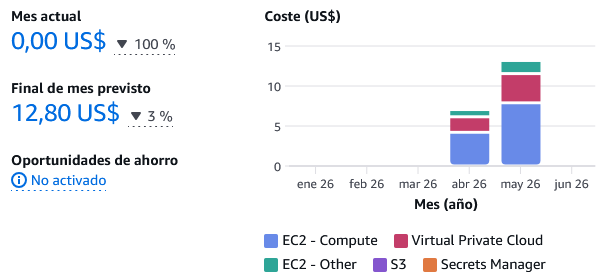
\includegraphics[width=\textwidth]{figuras/PrecioNube.png}
\caption{Estimación de costes para la instancia AWS EC2 t3.medium.}
\label{fig:aws_cost_estimation}
\end{figure}
\subsection{Resumen del Presupuesto y Coste Total}
La agregación de los costes de ingeniería, las licencias de software, la amortización de infraestructura local y el coste estimado de la infraestructura en AWS arroja la base imponible del proyecto (ver Tabla \ref{tab:presupuesto_total}).\vspace{0.5cm}

\begin{table}[htbp]
\centering
\caption{Resumen del presupuesto general del proyecto.}
\label{tab:presupuesto_total}
\begin{tabular}{p{10cm}p{3cm}}
\toprule
\textbf{Partida Presupuestaria} & \textbf{Importe (EUR)} \\
\midrule
Costes de Ingeniería (Mano de obra) & 10.880,00 \\
Costes de Software e Infraestructura & 19.650,00 \\
Coste estimado infraestructura AWS (2 meses) & 19,87 \\
\midrule
\textbf{Presupuesto Total General} & \textbf{30.549,87} \\
\bottomrule
\end{tabular}
\end{table}




\chapter{Conclusiones}
\label{cap:conclusiones}

El trabajo realizado en este TFM ha contribuido a ….. 

Las principales aportaciones y/o conclusiones que se extraen son …

Como acciones futuras o líneas de investigación abiertas e identificadas se proponen las siguientes:

\cleardoublepage
%---

%--- Insertar las Referencias Bibliográficas
{%
\renewcommand\bibname{Bibliografía}  % Cambiar el nombre a Castellano
\setstretch{1.1}
\renewcommand{\bibfont}{\normalfont\small}
\setlength{\biblabelsep}{0pt}
\setlength{\bibitemsep}{0.5\baselineskip plus 0.5\baselineskip}
\printbibliography[nottype=online]
\printbibliography[heading=subbibliography,title={Webseiten},type=online,prefixnumbers={@}]
}
\cleardoublepage
%---

%--- Insertar los Anexos
%\input{anexos/portada_anexo_esquemas_y_programas}
%\cleardoublepage
\appendix
\chapter{Anexo I: Código de la Solución}
\label{cap:anexo_codigo_solucion}

\section{Código de WinCC}
\definecolor{codegreen}{rgb}{0,0.6,0}
\definecolor{codegray}{rgb}{0.5,0.5,0.5}
\definecolor{codepurple}{rgb}{0,0,0.82}
\definecolor{backcolour}{rgb}{1,1,1}

\lstset{
    language=C,
    backgroundcolor=\color{backcolour},   
    commentstyle=\color{codegreen},
    keywordstyle=\color{magenta},
    numberstyle=\tiny\color{codegray},
    stringstyle=\color{codepurple},
    basicstyle=\ttfamily\scriptsize,
    breakatwhitespace=false,         
    breaklines=true,                 
    captionpos=b,                    
    keepspaces=true,                 
    numbers=left,                    
    numbersep=10pt,                  % Reducido a 10pt para que no se desplace demasiado al quitar el frame
    frame=single,                % Añade un borde muy fino
    framerule=0.2pt,
    xleftmargin=5pt,                % Añade margen izquierdo al bloque de color de fondo
    xrightmargin=5pt,                % Añade margen derecho al bloque de color de fondo
    aboveskip=0.75\baselineskip,
    belowskip=0.25\baselineskip,
    showspaces=false,                
    showstringspaces=false,
    showtabs=false,                  
    tabsize=2
}

\section{Código fuente}
\subsection{Filtrado de turbinas por estado y subestación}
\begin{lstlisting}
void AplicarFiltroPosicion(){

    int selValue, parkValue;
    int CANT_MOLINOS, i;
    int tagRun, tagEmg, tagPark, state;
    int match;

    // Variables de cuadricula
    int startX = 10;
    int startY = 0;
    int offsetX = 475;
    int offsetY = 220;
    int maxCols = 4;

    int currentX;
    int currentY;
    int colCount = 0;
    //Nombres de tags
    char tagNameRun[100];
    char tagNameEmg[100];
    char tagNamePark[100];
    char FP[50];

    // Guarda IDs de molinos que cumplen el filtro
    int validList[120];
    int validCount = 0;

    char* prefijoActual;

    currentX = startX;
    currentY = startY;
    // Obtener valores de filtros
    selValue = GetTagWord("HMI_Filtro_Molinos");
    parkValue = GetTagWord("HMI_Filtro_Parques");
    prefijoActual = "WTG";
    CANT_MOLINOS = 120;
    // Evaluar cada molino
    for (i = 1; i <= CANT_MOLINOS; i++) {
        sprintf(tagNameEmg, "%s%d.WTUR.TurSt.stVal", prefijoActual, i);
        sprintf(tagNamePark, "%s%d.LLNO.InSSet.setSrc", prefijoActual, i);

        tagEmg = GetTagWord(tagNameEmg);
        tagPark = GetTagWord(tagNamePark);

        switch (tagEmg) {
            case 0:
                state = 2;
                break;
            case 1:
            case 4:
                state = 3;
                break;
            case 2:
                state = 4;
                break;
            case 3:
                state = 5;
                break;
            case 5:
            case 7:
                state = 6;
                break;
            case 6:
                state = 7;
                break;
            default:
                if (tagEmg >= 10 && tagEmg <= 19) {
                    state = 8;
                } else {
                    state = -1;
                }
                break;
        }

        match = 0;
        if (parkValue == 1 || parkValue == tagPark) {
            if (selValue == 1 || selValue == state) {
                match = 1;
            }
        }

        if (match == 1) {
            validList[validCount] = i;
            validCount++;
        }
    }
    // Visualizar molinos que cumplen el filtro
    for (i = 1; i <= CANT_MOLINOS; i++) {
        sprintf(FP, "PW_%d", i);
        SetPropBOOL("20_WTG_Turbine_Overview.PDL", FP, "Visible", FALSE);
    }

    for (i = 0; i < validCount; i++) {
        int molinoID = validList[i];
        sprintf(FP, "PW_%d", molinoID);

        SetPropBOOL("20_WTG_Turbine_Overview.PDL", FP, "Visible", TRUE);
        SetPropDouble("20_WTG_Turbine_Overview.PDL", FP, "Left", currentX);
        SetPropDouble("20_WTG_Turbine_Overview.PDL", FP, "Top", currentY);

        colCount++;
        if (colCount >= maxCols) {
            currentX = startX;
            currentY += offsetY;
            colCount = 0;
        } else {
            currentX += offsetX;
        }
    }
}
\end{lstlisting}
\subsection{Filtrado de parques por estado y subestación}
\begin{lstlisting}
#include "apdefap.h" 
void AplicarFiltroParque(){ 

    //Variables
   
    int selValue, parkValue; 
    int CANT_VENTANAS = 22; 
    int i, k; 
    int match; 

    int tagParkBase;    // Parque del molino principal (TagPrefix)
    int currentPark;    // Parque del molino que estamos evaluando en el bucle k
    int baseID;         // ID numerico del molino principal 
    int currentID;      
    int rawStatus; 
    int state; 

    int startX = 10;    
    int startY = 0;     
    int offsetX = 475;  
    int offsetY = 225;  
    int maxCols = 4; 
    
    int currentX = startX; 
    int currentY = startY; 
    int colCount = 0;  

    char FP[50];  
    char* prefijoVentana; 
    char tagName[150]; 

    //Leer valores de filtros
    selValue = GetTagWord("HMI_Filtro_Molinos"); 
    parkValue = GetTagWord("HMI_Filtro_Parques"); 

  
    // Evaluar cada ventana de imagen (cada una con un parque base diferente)

    for (i = 1; i <= CANT_VENTANAS; i++) { 
        match = 0; 
        
        sprintf(FP, "PK_%d", i); 
        
        // LEEMOS EL TAG PREFIX
        prefijoVentana = GetPropChar("21_WTG_Park_Overview.PDL", FP, "TagPrefix"); 
        
        if (prefijoVentana != NULL && strlen(prefijoVentana) > 0) { 
            
            // Leemos el parque del molino base para referencia
            sprintf(tagName, "%s.LLNO.SubSt.setSrc", prefijoVentana); 
            tagParkBase = GetTagWord(tagName); 
            
            // Leemos el ID numerico base
            sprintf(tagName, "%s.LLNO.UnitID.setSrc", prefijoVentana); 
            baseID = GetTagWord(tagName); 

            if (baseID > 0) {
                // BUCLE K: Comprobamos el molino base (0), el +1 y el +2
                for (k = 0; k < 3; k++) { 
                    currentID = baseID + k; 

                    // 1. Obtener parque del molino actual (k) para ver si esta en el parque filtrado
                    if (k == 0) {
                        currentPark = tagParkBase;
                    } else {
                        sprintf(tagName, "WTG%d.LLNO.SubSt.setSrc", currentID); 
                        currentPark = GetTagWord(tagName);
                    }

                    // FILTRO DE PARQUE: El molino 'k' debe pertenecer al parque seleccionado
                    if (parkValue == 1 || parkValue == currentPark) {
                        
                        // 2. Leer estado del molino 'k'
                        if (k == 0) {
                            sprintf(tagName, "%s.WTUR.TurSt.stVal", prefijoVentana);
                        } else {
                            sprintf(tagName, "WTG%d.WTUR.TurSt.stVal", currentID);
                        }
                        rawStatus = GetTagWord(tagName); 

                        // 3. Maquina de estados interna 
                        switch (rawStatus) { 
                            case 0: state = 2; break; // Stopped 
                            case 1: 
                            case 4: state = 3; break; // Starting o Shutting down 
                            case 2: state = 4; break; // Running 
                            case 3: state = 5; break; // Paused 
                            case 5: 
                            case 7: state = 6; break; // Emergency stop o Fault 
                            case 6: state = 7; break; // Maintenance 
                            default: 
                                if (rawStatus >= 10 && rawStatus <= 19) { 
                                    state = 8; // Communication Error 
                                } else { 
                                    state = -1; 
                                } 
                                break; 
                        } 

                        //filtro estado
                        if (selValue == 1 || selValue == state) { 
                            match = 1;  
                            break; // Si uno de los tres cumple, ya no hace falta mirar mas
                        } 
                    }
                } 
            } 
        } 
        
       
        // Visualizacion de ventanas: Si 'match' es 1, esta ventana se muestra en la cuadricula, si no se oculta
    
        if (match == 1) { 
            SetPropDouble("21_WTG_Park_Overview.PDL", FP, "Left", currentX); 
            SetPropDouble("21_WTG_Park_Overview.PDL", FP, "Top", currentY);  
            SetPropBOOL("21_WTG_Park_Overview.PDL", FP, "Visible", TRUE); 
            
            colCount++; 
            if (colCount >= maxCols) { 
                currentX = startX; 
                currentY += offsetY; 
                colCount = 0; 
            } else { 
                currentX += offsetX; 
            } 
        } else { 
            SetPropBOOL("21_WTG_Park_Overview.PDL", FP, "Visible", FALSE); 
        } 
    } 
}
\end{lstlisting}
\subsection{Navegación menu}
\begin{lstlisting}
Sub MenuNavigation(Byval menuItem)
Dim myScreen : myScreen =menuItem.userData
HMIRuntime.Screens(BaseScreenName).ScreenItems("img_GUI").TagPrefix=""
HMIRuntime.Screens(BaseScreenName).ScreenItems("img_GUI").PictureName=myScreen

If myScreen ="13_SYS_Alarms" Then 
	HMIRuntime.Screens(BaseScreenName).ScreenItems("img_alarm").PictureName="DiagLog"
Else
	HMIRuntime.Screens(BaseScreenName).ScreenItems("img_alarm").PictureName="AlarmLog"
End If


End Sub
\end{lstlisting}
\section{Código de IIoT}

\begin{lstlisting}[language=bash]
sudo apt update
sudo apt install docker.io docker-compose -y
sudo systemctl start docker
sudo systemctl enable docker
\end{lstlisting}

% Tip: He cambiado temporalmente a lenguaje=YAML para que el resaltado del compose sea correcto
\begin{lstlisting}[language=XML]
version: '3.8'

services:
  mosquitto:
    image: eclipse-mosquitto:latest
    container_name: broker_mqtt
    ports:
      - "1883:1883"
    volumes:
      - ./mosquitto/config/mosquitto.conf:/mosquitto/config/mosquitto.conf
    restart: always

  influxdb:
    image: influxdb:2.7
    container_name: base_datos
    ports:
      - "8086:8086"
    volumes:
      - ./influxdb_data:/var/lib/influxdb2
    restart: always

  nodered:
    image: nodered/node-red:latest
    container_name: puente_nodered
    ports:
      - "1880:1880"
    volumes:
      - ./nodered_data:/data
    restart: always

  grafana:
    image: grafana/grafana:latest
    container_name: graficos_web
    ports:
      - "3000:3000"
    volumes:
      - ./grafana_data:/var/lib/grafana
    restart: always

\end{lstlisting}

\begin{lstlisting}[language=bash]
sudo docker-compose up -d
\end{lstlisting}

\vspace{1cm}



\chapter{Anexo II: Planos}
\label{cap:Planos}

La incorporación de anexos es opcional y se justifica si su lectura no es indispensable para la correcta comprensión de la Memoria. Por ejemplo, puede ser conveniente incluir un Manual de Usuario, un Manual de Instalación, una Hoja de Especificaciones, Planos, Código, etc


\chapter{Anexo III: Banco de Pruebas y Validación del Sistema}
\label{cap:Pruebas}

\section{Gemelo funcional de aerogeneradores}
\begin{figure}[htbp]
    \centering
    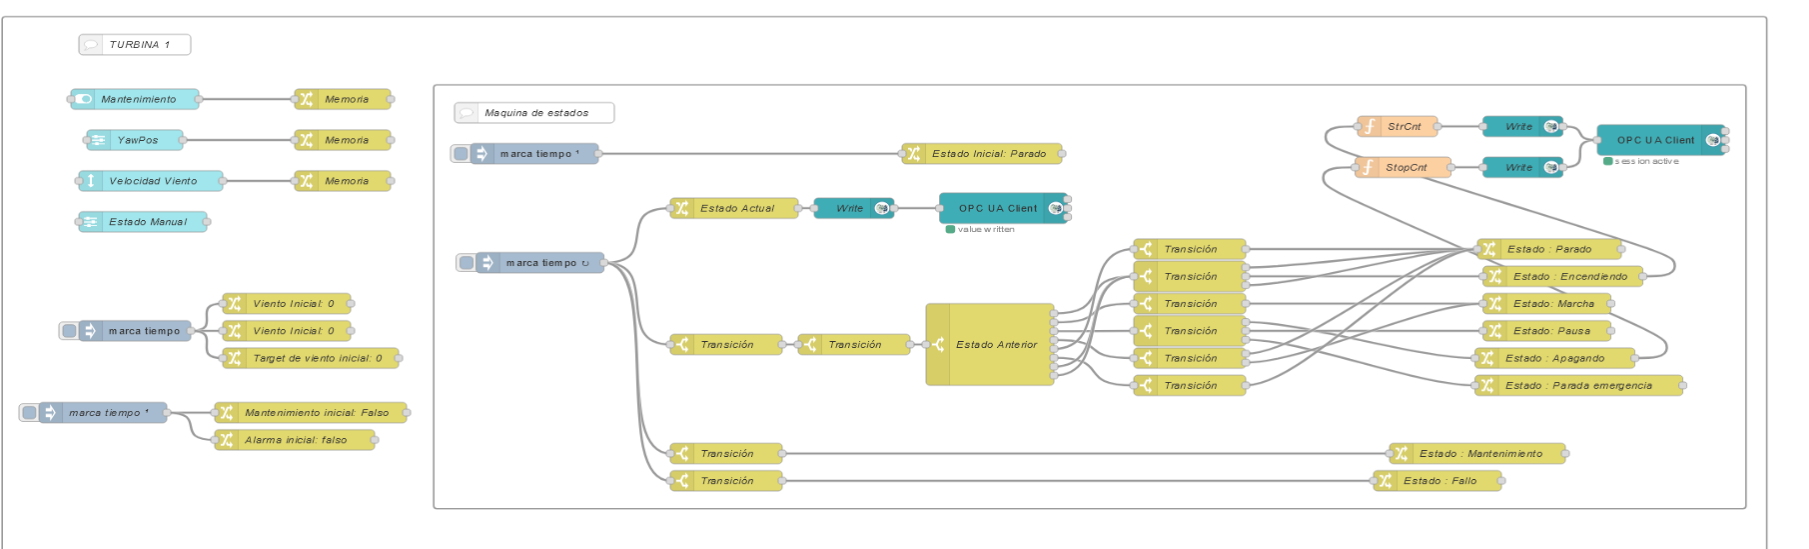
\includegraphics[width=\textwidth]{figuras/maquinaestados.png}
    \caption{Maquina de estados del modelo de simulación de aerogeneradores.}
    \label{fig:modelo_simulacion_aerogenerador}
\end{figure}
\begin{figure}[htbp]
    \centering
    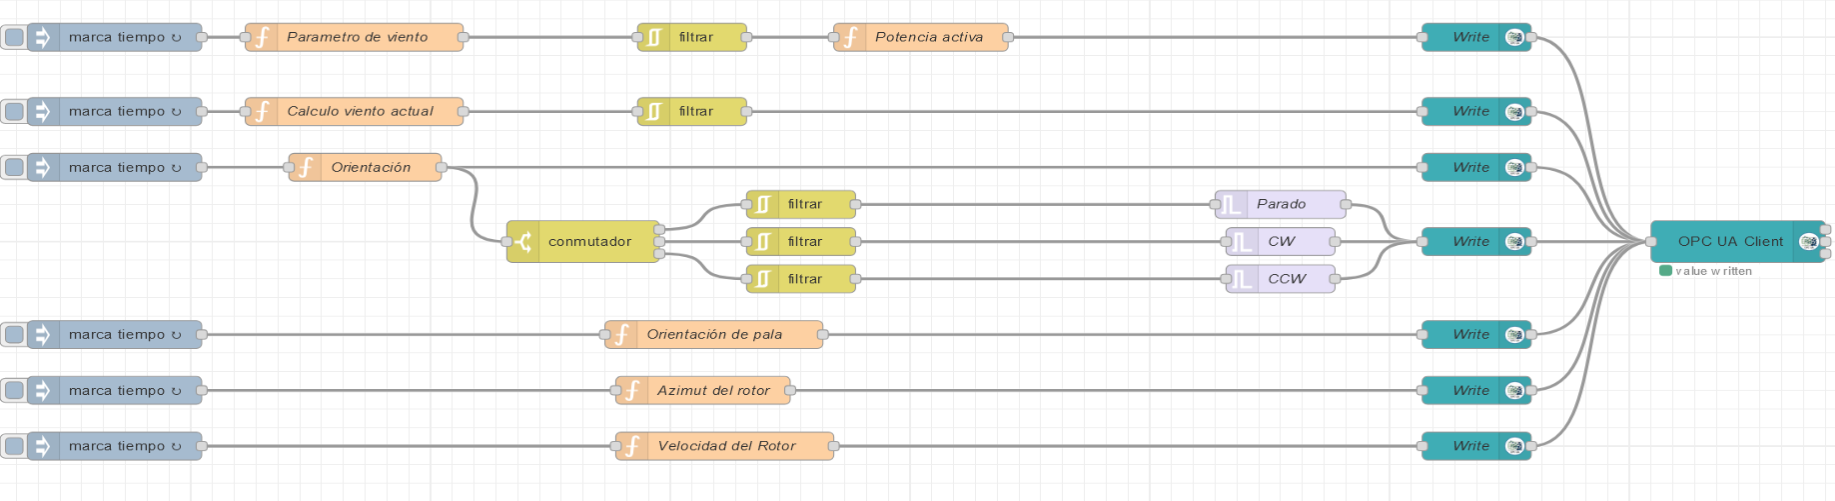
\includegraphics[width=\textwidth]{figuras/CalculoAnalogico.png}
    \caption{Cálculo analógico de variables de interés.}
    \label{fig:modelo_simulacion_aerogenerador}
\end{figure}
\begin{figure}[htbp]
    \centering
    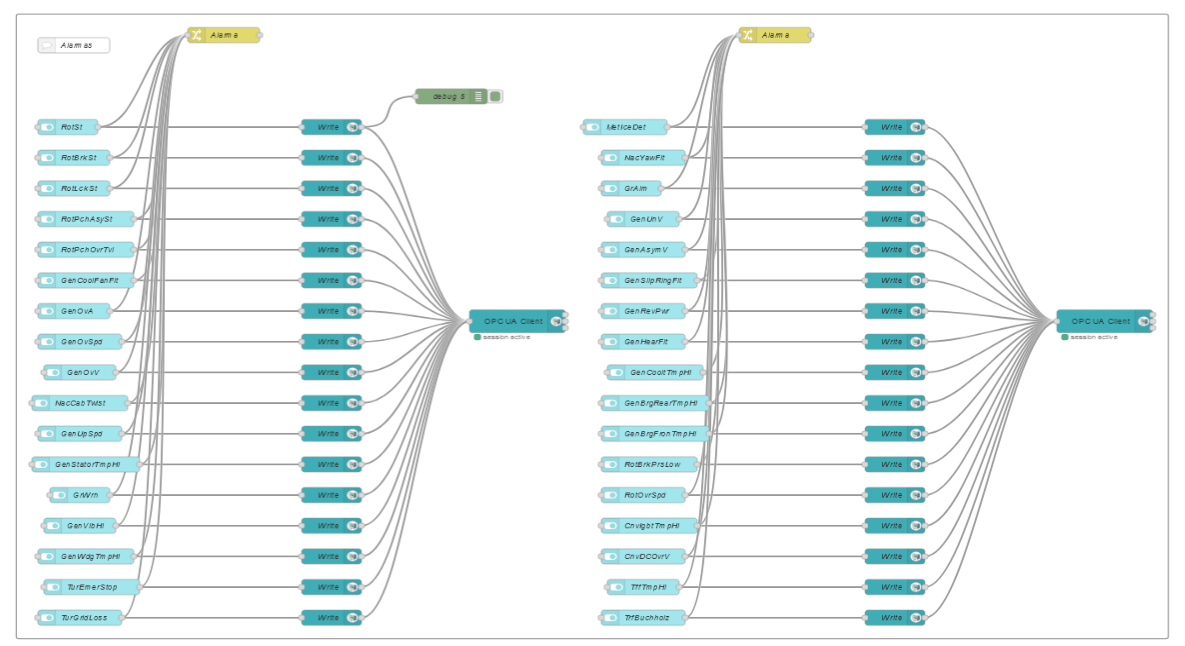
\includegraphics[width=\textwidth]{figuras/Alarmas.png}
    \caption{Control de alarmas y eventos en el modelo de simulación.}
    \label{fig:modelo_simulacion_aerogenerador}
\end{figure}
\begin{figure}[htbp]
    \centering
    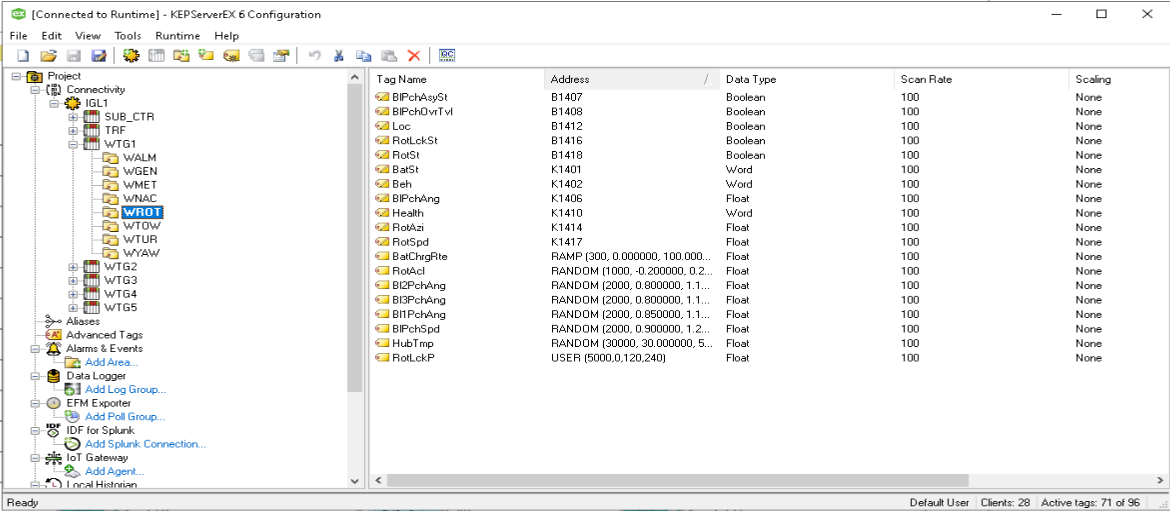
\includegraphics[width=\textwidth]{figuras/SimKepServer.png}
    \caption{Control de alarmas y eventos en el modelo de simulación.}
    \label{fig:modelo_simulacion_aerogenerador}
\end{figure}

\chapter{Anexo IV: Manual de Usuario}
\label{cap:Manual}
En este anexo se incluye un manual de usuario para la solución desarrollada. Este manual está dirigido a los usuarios finales que interactuarán con el sistema, proporcionando instrucciones claras y detalladas sobre cómo utilizar las funcionalidades implementadas. Se incluyen capturas de pantalla, descripciones de cada función y pasos para realizar tareas comunes dentro del sistema.

La base física de esta jerarquía se fundamenta en el siguiente elemento:\par

\subsection{Nivel 0: Marco Base (\texttt{00\_Main\_Interface})}
Representa la interfaz matriz o Nivel 0 del SCADA (Figura \ref{fig:00_main_interface}). En lugar de ejecutar transiciones de pantalla completa, esta plantilla actúa como un contenedor estático  que alberga el menú de navegación principal e implementa dos \textit{Picture Windows} independientes.\par

La ventana de trabajo central ocupa la mayor parte de la pantalla y constituye el área de visualización dinámica donde se cargan todas las interfaces operativas (Niveles 1 a 4). Paralelamente, la ventana de alarmas inferiores es un espacio de menores dimensiones anclado de forma fija en el pie de página, cuya única función es garantizar la supervisión ininterrumpida de los eventos críticos independientemente de la profundidad de navegación del usuario.
\FloatBarrier
\subsection{Nivel 1: Supervisión Global}
\label{sec:nivel_1_overview}
\subsubsection{Vista General de aerogeneradores (\texttt{10\_WTG\_Overview})}
La pantalla \texttt{10\_WTG\_Overview} actúa como el nodo principal de enrutamiento dinámico del SCADA. Su diseño optimiza la navegación hacia los niveles inferiores mediante tres mecanismos clave integrados en su cabecera.\par

Por un lado, se ha implementado un sistema de filtrado mediante dos selectores desplegables (Figura \ref{fig:interfaz_grafica_selector}) que acotan la información visualizada, actualizando los aerogeneradores mostrados sin necesidad de realizar transiciones a otras pantallas ( Algoritmo \ref{alg:filtrado_dinamico}, vease la función \texttt{AplicarFiltroPosicion()} en el Anexo \ref{cap:anexo_codigo_solucion}).\par

Por otro lado, como se observa en la figura \ref{fig:interfaz_grafica_park} un selector central gestiona el archivo alojado en el \textit{Picture Window} de trabajo. Permite alternar instantáneamente entre la telemetría individual de las turbinas (\texttt{20\_WTG\_Turbine\_Overview.pdl}) y la vista de datos por parques (\texttt{21\_WTG\_Park\_Overview.pdl}).\par

Finalmente, como se muestra en la figura \ref{fig:interfaz_grafica} una matriz superior de indicadores discretos organizados por parques representa el estado de cada aerogenerador. Seleccionar uno de ellos actúa como acceso directo al Nivel 4 (\texttt{40\_WTG\_Gen}), omitiendo pasos intermedios e inyectando automáticamente el \textit{Tag Prefix} correspondiente para cargar los datos de la máquina seleccionada.\par


\label{sec:nivel_1_subestacion}
Esta pantalla actúa como un contenedor especializado para la visualización de la infraestructura eléctrica del parque. Arquitectónicamente, se ha diseñado como una interfaz intermedia que alberga un único \textit{Picture Window} destinado a cargar los diversos diagramas unifilares (\textit{Single Line Diagrams}).\par

La decisión de no integrar estos esquemas directamente en la pantalla raíz (\texttt{00\_Main\_Interface}) y emplear este encapsulamiento responde a dos criterios técnicos fundamentales, por un lado, la gestión de la visualización y desplazamiento de diagramas eléctricos complejos (\textit{scrolling}), y por otro, el aislamiento de variables mediante \textit{Tag Prefixes} para evitar interferencias con el entorno principal del SCADA.\par
\subsubsection{Interfaz de monitorización, alarmas y tendencias (\texttt{12\_MET\_Station}, \texttt{13\_SYS\_Alarms} y \texttt{14\_SYS\_Trends})}

Como complemento indispensable a las vistas generales de generación y evacuación de potencia, se han integrado en el Nivel 1 tres interfaces dedicadas a la monitorización ambiental, el diagnóstico del historial de fallos y el soporte operativo del entorno SCADA. Estas pantallas, identificadas bajo los archivos \texttt{12\_MET\_Station.pdl}, \texttt{13\_SYS\_Alarms.pdl} y \texttt{14\_SYS\_Trends\_Interface.pdl}, aseguran que el operador mantenga una conciencia situacional periférica sobre las variables externas, las condiciones meteorológicas y el estado de salud del propio sistema de adquisición de datos sin necesidad de descender individualmente en la jerarquía de cada aerogenerador.\par

\FloatBarrier

\section{Interfaz Gráfica: Nivel 2 - Supervisión Global por Activos}
\label{sec:nivel2_scada}

Habiendo definido en el Nivel 1 las áreas macroscópicas y los marcos contenedores del sistema \cite{7.6.3}, el Nivel 2 se constituye como el primer escalón de desglose y segregación funcional del parque eólico. Siguiendo de forma estricta el patrón de diseño e ingeniería de nomenclatura definido en la Ecuación~\ref{eq:nomenclatura}, todas las pantallas pertenecientes a este nivel adoptan el prefijo numérico \texttt{2X}.

\subsection{Definición y Catálogo de Pantallas del Nivel 2}
Con el propósito de gestionar de forma eficiente la telemetría de los 120 aerogeneradores y el flujo energético de las 9 subestaciones de transformación y evacuación \cite{7.3}, se han diseñado e implementado las siguientes interfaces gráficas en formato \texttt{.pdl} dentro del entorno de desarrollo SIMATIC WinCC V8.1 \cite{29}:

\begin{itemize}
    \item \textbf{\texttt{20\_WTG\_Turbine\_Overview.pdl} (Malla de Turbinas Individuales):} Pantalla orientada a objetos que actúa como un contenedor dinámico en tiempo de ejecución (\textit{Runtime}) \cite{575}. Alberga un total de 120 ventanas de imagen (\textit{Picture Windows}) indexadas numéricamente (\texttt{PW\_1} a \texttt{PW\_120}) \cite{1748, 1763}. Su propósito operativo es renderizar de forma compacta y ordenada los \textit{faceplates} de monitorización rápida de cada activo físico en base al estado de los filtros globales de la aplicación.
    \item \textbf{\texttt{21\_WTG\_Park\_Overview.pdl} (Supervisión Agregada por Clúster):} Interfaz gráfica de abstracción técnica superior orientada a la consolidación de datos e indicadores clave de rendimiento (KPIs) por subestaciones o zonas lógicas \cite{1167, 1279}. Esta vista unifica variables totalizadas del clúster (potencia activa agregada, velocidad media del viento sectorial y balance de activos en estado de alarma o mantenimiento) \cite{1241, 1280}.
    \item \textbf{\texttt{22\_SUB\_SLD\_General.pdl} (Diagrama Unifilar General del Complejo):} Representación estática y dinámica del esquema unifilar (\textit{Single Line Diagram} - SLD) macroscópico del parque eólico \cite{1169, 1200}. Visualiza de forma unificada las líneas de barras comunes del complejo y el estado de los interruptores automáticos (\texttt{XCBR}) y seccionadores (\texttt{XSWI}) principales de evacuación hacia la red de transporte nacional eléctrica \cite{855, 887}.
    \item \textbf{\texttt{23\_SYS\_TrendTime.pdl} (Tendencias Temporales de Proceso):} Pantalla especializada que integra el control nativo \textit{WinCC Online Trend Control} \cite{1804}. Permite al operador analizar de forma gráfica series temporales continuas de variables de proceso críticas (e.g., velocidad angular del rotor \texttt{WROT.RotSpd} o temperatura del estator \texttt{WGEN.Tmp}) \cite{1064, 1103}.
    \item \textbf{\texttt{24\_SYS\_XYTrend.pdl} (Gráficas de Diagnóstico Analítico X-Y):} Interfaz dedicada a la monitorización predictiva del rendimiento aerodinámico \cite{362, 441}. Su función primordial es cruzar la velocidad instantánea del viento local medida por el anemómetro de góndola (\texttt{WMET.WndSpd}) frente a la potencia activa final inyectada en bornes (\texttt{WGEN.W}) \cite{788, 1848, 1856}. De este modo, se genera dinámicamente en pantalla la curva de potencia real del activo, permitiendo evaluar desviaciones frente a la curva teórica del fabricante.
\end{itemize}

\subsection{Lógica Matemática de Ordenación en Cuadrícula y Filtrado}
Para evitar que el operador sufra de saturación de información ante 120 activos simultáneos, la pantalla \texttt{20\_WTG\_Turbine\_Overview} ejecuta un algoritmo dinámico en lenguaje ANSI-C a través del subsistema \textit{Global Scripts} \cite{586, 1285}. El script lee los estados lógicos de los filtros seleccionados por el usuario y posiciona vectorialmente en una matriz bidimensional los faceplates válidos.

Sea $i \in \{1, 2, \dots, N_{total}\}$ el índice único que identifica a cada aerogenerador, donde $N_{total} = 120$ \cite{1751}. Definimos las variables de configuración espacial inicial en el lienzo gráfico como:
\begin{itemize}
    \item $X_{start} = 10 \text{ px}$ \quad (Margen izquierdo de la cuadrícula) \cite{1744}
    \item $Y_{start} = 0 \text{ px}$ \quad (Margen superior de la cuadrícula) \cite{1744}
    \item $\Delta X = 475 \text{ px}$ \quad (Ancho del faceplate más el espaciado horizontal) \cite{1745}
    \item $\Delta Y = 220 \text{ px}$ \quad (Alto del faceplate más el espaciado vertical) \cite{1745}
    \item $C_{max} = 4$ \quad (Número máximo de columnas permitidas por fila) \cite{1745}
\end{itemize}

Introduciendo la variable indexada de conteo de activos válidos que han superado con éxito las condiciones de filtrado cromo-operativo como $k$ (inicializada en $k = 0$), la posición espacial final de la esquina superior izquierda (coordenadas \textit{Left} y \textit{Top} de WinCC) para cada ventana de imagen visible se calcula de forma unívoca mediante las siguientes funciones de mapeo discreto:

\begin{equation}
    X_{pos}(k) = X_{start} + \left( k \pmod{C_{max}} \right) \cdot \Delta X
    \label{eq:pos_x}
\end{equation}

\begin{equation}
    Y_{pos}(k) = Y_{start} + \left\lfloor \frac{k}{C_{max}} \right\rfloor \cdot \Delta Y
    \label{eq:pos_y}
\end{equation}

Donde la operación módulo ($\pmod{}$) restringe el crecimiento en el eje horizontal asegurando la matriz de 4 columnas, y la función piso matemático ($\lfloor \rfloor$) incrementa de forma discreta la altura del renglón cada vez que el contador $k$ supera un múltiplo exacto de $C_{max}$ \cite{1769}. 

\subsection{Mecanismo de Integración en el Marco Base (Runtime)}
En concordancia con la arquitectura multipuesto de alta disponibilidad y virtualización industrial mediante el servicio SIVaaS implementado \cite{600, 648}, el flujo de navegación prohíbe las transiciones de pantalla completa tradicionales para mitigar la sobrecarga de intercambio de memoria en las estaciones cliente \cite{1179}. 

Como se ilustra en la estructura del proyecto, las interfaces del Nivel 2 se cargan bajo demanda de forma interna modificando dinámicamente la propiedad \texttt{PictureName} del objeto \texttt{PictureWindow} central configurado en el marco maestro estático \texttt{00\_Main\_Interface.pdl} \cite{1184, 1185}. La ventana inferior de avisos críticos de \textit{Alarm Logging} permanece fija en la zona del pie de página de forma persistente, garantizando que el operador no pierda la conciencia situacional ni la trazabilidad de eventos del nodo \texttt{WALM} de la planta durante el desplazamiento por el Nivel 2 \cite{1186, 1353, 1414}.
\chapter{Anexo V: Tablas de variables}
\label{cap:Tablas_Variab}

\section{Introducción}
En este anexo se incluyen las tablas de variables utilizadas en la solución desarrollada. Estas tablas detallan los nombres, tipos y descripciones de las variables empleadas en el sistema, proporcionando una referencia completa para el mantenimiento y la configuración del SCADA.
\section{Variables de Aerogeneradores}
\begin{longtable}[t]{p{2cm} p{3cm} p{1cm} p{7cm}}
    \toprule
    \toprule
    \multicolumn{4}{c}{\textbf{Estructuras de Variables de nivel 2 y 3}} \\
    \midrule
    Nombre & Dato & CDC & Descripción\\
    \midrule
    \endfirsthead

    \toprule
    \multicolumn{4}{c}{\textbf{Estructuras de Variables de nivel 2 y 3 (continuación)}} \\
    \midrule
    Nombre & Dato & CDC & Descripción\\
    \midrule
    \endhead

    \midrule
    \multicolumn{4}{r}{Continúa en la siguiente página}\\
    \endfoot

    \bottomrule
    \bottomrule
    \\
    \caption{Estructuras de variables de nivel 2 y 3 según norma IEC 61400-25-2.}
    \label{tab:equipo3}\\
    \endlastfoot

        LLN0 & \textit{NamPlt} & DPL & Placa de identificación con datos de nombre y fabricante.\\
            & \textit{Diag} & SPS & Indicación de diagnóstico general del dispositivo.\\
            & \textit{MltLev} & SPS & Indicación de nivel múltiple o estado multinivel resumido.\\
            & \textit{InSSet} & ZID & Identificador de parque eólico.\\
            & \textit{SubSt} & ZID & Identificador de subestación.\\
        \midrule
        LPHD & \textit{PhyNam} & DPL & Nombre físico del dispositivo lógico o equipo asociado.\\
            & \textit{PhyHealth} & INS & Estado de salud física del dispositivo.\\
            & \textit{Proxy} & SPS & Indica operación en modo proxy o representación remota.\\
            & \textit{Sim} & SPS & Indica si el dispositivo está en modo simulación.\\
            & \textit{PwrUp} & INS & Estado asociado al encendido/arranque del dispositivo.\\
            & \textit{WrmStr} & INS & Estado de arranque en caliente o reinicio de servicio.\\
            & \textit{WacTrg} & Valor de 32 bits sin signo & Contador o valor de activación de mantenimiento/servicio.\\
            & \textit{WdgAct} & SPS & Estado de actividad del watchdog del dispositivo.\\
            & \textit{OutOv} & SPS & Estado de anulación (override) de salidas.\\
            & \textit{OpTmh} & INS & Tiempo acumulado de operación del dispositivo (horas).\\
        \midrule
        WALM & \textit{NamPlt} & DPL & Placa de identificación del nodo lógico de alarmas.\\
            & \textit{GrAlm} & SPS & Indicador de alarma general activa.\\
            & \textit{GrWrn} & SPS & Indicador de advertencia general activa.\\
            & \textit{AlmCnt} & INS & Contador total de alarmas registradas.\\
            & \textit{WrnCnt} & INS & Contador total de advertencias registradas.\\
            & \textit{GenOvSpd} & SPS & Alarma de sobrevelocidad del generador.\\
            & \textit{GenInSpd} & SPS & Alarma de velocidad insuficiente del generador.\\
            & \textit{GenStatorTmpHi} & SPS & Alarma de alta temperatura del estator del generador.\\
            & \textit{GenBrgFronTmpHi} & SPS & Alarma de alta temperatura en rodamiento frontal del generador.\\
            & \textit{GenBrgRearTmpHi} & SPS & Alarma de alta temperatura en rodamiento trasero del generador.\\
            & \textit{GenCoolTmpHi} & SPS & Alarma de alta temperatura del sistema de refrigeración del generador.\\
            & \textit{GenOvV} & SPS & Alarma de sobretensión del generador.\\
            & \textit{GenUnV} & SPS & Alarma de subtensión del generador.\\
            & \textit{GenOvA} & SPS & Alarma de sobrecorriente del generador.\\
            & \textit{GenAsymV} & SPS & Alarma de asimetría de tensión del generador.\\
            & \textit{GenRevPwr} & SPS & Alarma de potencia inversa del generador.\\
            & \textit{GenVibHi} & SPS & Alarma de vibración alta del generador.\\
            & \textit{GenCoolFanFlt} & SPS & Alarma de fallo de ventilador de refrigeración del generador.\\
            & \textit{GenSlipRingFlt} & SPS & Alarma de fallo en anillos rozantes del generador.\\
            & \textit{GenHeaFlt} & SPS & Alarma de fallo del calentador del generador.\\
            & \textit{TurEmerStop} & SPS & Alarma de parada de emergencia de la turbina.\\
            & \textit{TurGridLoss} & SPS & Alarma de pérdida de red eléctrica.\\
            & \textit{RotOvrSpd} & SPS & Alarma de sobrevelocidad del rotor.\\
            & \textit{RotPitcAsym} & SPS & Alarma de asimetría de pitch entre palas.\\
            & \textit{RotBrkPrsLow} & SPS & Alarma de presión baja en freno del rotor.\\
            & \textit{GenWdgTmpHi} & SPS & Alarma de alta temperatura en devanados del generador.\\
            & \textit{GenBrgTmpHi} & SPS & Alarma de alta temperatura en rodamientos del generador.\\
            & \textit{CnvDCOvrV} & SPS & Alarma de sobretensión en bus DC del convertidor.\\
            & \textit{CnvIgbtTmpHi} & SPS & Alarma de alta temperatura en IGBT del convertidor.\\
            & \textit{NacCabTwist} & SPS & Alarma de retorcimiento excesivo de cables en góndola.\\
            & \textit{NacYawFlt} & SPS & Alarma de fallo del sistema de Yaw de góndola.\\
            & \textit{TrfBuchholz} & SPS & Alarma Buchholz del transformador.\\
            & \textit{TrfTmpHi} & SPS & Alarma de alta temperatura del transformador.\\
            & \textit{MetIceDet} & SPS & Detección de hielo por sistema meteorológico.\\
        \midrule
        WGEN & \textit{GnSt} & INS & Estado operativo del generador (ej. Desconectado, Conectado, Fallo)\\
            & \textit{OpTmh} & INS & Tiempo de operación total del generador (horas)\\
            & \textit{Spd} & MV & Velocidad de giro del generador (RPM)\\
            & \textit{Hz} & MV & Frecuencia eléctrica del generador\\
            & \textit{W} & MV & Potencia activa generada (Bornes)\\
            & \textit{VAr} & MV & Potencia reactiva generada (Bornes)\\
            & \textit{CosPhi} & MV & Factor de potencia (cos $\phi$)\\
            & \textit{Tmp} & MV & Temperatura general del estator / devanados\\
            & \textit{BrgFronTmp} & MV & Temperatura del rodamiento frontal (Lado acople/Rotor)\\
            & \textit{BrgRearTmp} & MV & Temperatura del rodamiento trasero (Lado no acople)\\
            & \textit{CoolTmp} & MV & Temperatura del fluido o aire de refrigeración del generador\\
            & \textit{HeaSt} & SPS & Estado del calentador del generador (anticondensación)\\
            & \textit{Slip} & MV & Deslizamiento del generador (típico en asíncronos doblemente alimentados)\\
        \midrule
        WMET & \textit{WndSpd} & MV & Velocidad del viento.\\
            & \textit{WndDir} & MV & Dirección del viento.\\
            & \textit{EnvTmp} & MV & Temperatura ambiente.\\
            & \textit{EnvPres} & MV & Presión atmosférica.\\
            & \textit{EnvHum} & MV & Humedad ambiental.\\
            & \textit{IceDet} & SPS & Detección de hielo.\\
            & \textit{Precip} & MV & Precipitación.\\
            & \textit{Visib} & MV & Visibilidad.\\
        \midrule
        WNAC & \textit{NacTmp} & MV & Temperatura en la góndola.\\
            & \textit{NacHum} & MV & Humedad en la góndola.\\
            & \textit{YawPos} & MV & Posición angular del sistema de orientación (Yaw).\\
            & \textit{YawErr} & MV & Error de orientación respecto a la consigna de Yaw.\\
            & \textit{CabTws} & MV & Estado o magnitud del retorcimiento de cables (cable twist).\\
            & \textit{YawSt} & INS & Estado del sistema de orientación Yaw.\\
            & \textit{NacVib} & MV & Nivel de vibración de la góndola.\\
            & \textit{WlkHtz} & SPS & Estado de habilitación o enclavamiento asociado al nodo de góndola.\\
        \midrule
        WREP & \textit{TmsRpt} & INS & Intervalo de tiempo: duración del reporte en segundos (ej. 600 para 10 min).\\
            & \textit{WAvg} & MV & Potencia media: promedio de potencia activa en el intervalo.\\
            & \textit{WMax} & MV & Potencia máxima: el pico de potencia alcanzado en el intervalo.\\
            & \textit{WMin} & MV & Potencia mínima: el valor más bajo de potencia en el intervalo.\\
            & \textit{WStd} & MV & Desviación estándar de W: indica la estabilidad de la generación.\\
            & \textit{WsAvg} & MV & Viento medio: velocidad de viento promedio (10 min).\\
            & \textit{WsMax} & MV & Viento máximo: ráfaga máxima detectada en el intervalo.\\
            & \textit{RptRst} & SPC & Reset de reporte: comando para forzar el cierre del intervalo actual.\\
        \midrule
        WROT & \textit{RotSpd} & MV & Velocidad de rotación\\
            & \textit{RotAcl} & MV & Aceleración de rotación\\
            & \textit{RotAzi} & MV & Posición de rotación\\
            & \textit{RotSt} & MV & Estado de rotación\\
            & \textit{RotLckP} & MV & Posición de bloqueo del rotor\\
            & \textit{RotLckSt} & MV & Estado de bloqueo del rotor\\
            & \textit{Bl1PchAng} & MV & Ángulo de pala A\\
            & \textit{Bl2PchAng} & MV & Ángulo de pala B\\
            & \textit{Bl3PchAng} & MV & Ángulo de pala C\\
            & \textit{BlPchAngRef} & MV & Ángulo de referencia de pala\\
            & \textit{BlPchOvrTvl} & MV & Viaje excesivo de pala\\
            & \textit{BlPchAng} & MV & Estado de pitch control\\
            & \textit{BlPchSpd} & MV & Presión hidráulica\\
            & \textit{HubTmp} & MV & Estado hidráulico\\
            & \textit{BlPchAsySt} & MV & Voltaje de batería\\
            & \textit{BatChrgRte} & MV & Tasa de carga de batería\\
            & \textit{BatSt} & MV & Estado de batería\\
            & \textit{HubTmp} & MV & Temperatura del buje\\
        \midrule
        WTOW & \textit{NacPos} & MV & Posición de la góndola respecto a la torre.\\
            & \textit{TowVib} & MV & Nivel de vibración de la torre.\\
            & \textit{TowInc} & MV & Inclinación de la torre.\\
            & \textit{GndTmp} & MV & Temperatura ambiente a nivel de suelo.\\
            & \textit{GndHum} & MV & Humedad relativa a nivel de suelo.\\
            & \textit{IntTmp} & MV & Temperatura interior en torre/gabinete asociado.\\
            & \textit{Plt} & SPC & Comando de plataforma o acción de mantenimiento asociada a torre.\\
            & \textit{LkrSt} & SPS & Estado del enclavamiento o bloqueo de acceso de torre.\\
        \midrule
        WTUR & \textit{AvlTmRs} & TMS & Tiempo de disponibilidad de la turbina\\
            & \textit{OpTmRs} & TMS & Tiempo de operación\\
            & \textit{StrCnt} & WTC & Número de arranques de turbina\\
            & \textit{StopCnt} & WTC & Número de paradas de turbina\\
            & \textit{TotWh} & WTC & Producción total de energía activa (neta)\\
            & \textit{TotVArh} & WTC & Producción total de energía reactiva (neta)\\
            & \textit{DmdWh} & BCR & Demanda de energía activa (real)\\
            & \textit{DmdVArh} & BCR & Demanda de energía reactiva\\
            & \textit{SupWh} & BCR & Suministro de energía activa (real)\\
            & \textit{SupVArh} & BCR & Suministro de energía reactiva\\
            & \textit{TurSt} & SPS & Estado de la turbina\\
            & \textit{W} & MV & Generación de potencia activa\\
            & \textit{VAr} & MV & Generación de potencia reactiva\\
            & \textit{SetTurOp} & SPC & Comando de operación de la turbina eólica\\
            & \textit{VArOvW} & SPC & Prioridad de reactiva sobre activa\\
            & \textit{VArRefPri} & SPC & Comando de prioridad de consigna reactiva\\
            & \textit{DmdW} & APC & Consigna de generación de potencia activa\\
            & \textit{DmdVAr} & APC & Consigna de generación de potencia reactiva\\
            & \textit{DmdPF} & APC & Consigna de factor de potencia de turbina\\
        \midrule
        WYAW & \textit{YawSt} & INS & Estado del Yaw: 0:Parado, 1:Girando, 2:Frenado, 3:Desenrrollando cables.\\
            & \textit{YawTrq} & MV & Torque de orientación: fuerza que están haciendo los motores para girar contra el viento.\\
            & \textit{MotA} & MV & Corriente de los motores: amperaje consumido por los motores de Yaw (detecta bloqueos).\\
            & \textit{YawDrp} & MV & Desviación de consigna: qué tan rápido está corrigiendo el ángulo el sistema.\\
            & \textit{YawStop} & SPC & Comando de parada: para detener el giro manualmente desde WinCC.\\
    \midrule
\end{longtable}

\section{Variables de Transformadores}
\section{Variables de Subestaciones}
\newpage
\mbox{}

\end{document}
